\chapter{Solutions to the exercises}
\label{ch:solutions}

\section*{Exercise \ref{Ex:1.1}: Manipulating spinor indices}
\label{Prob:1.1}
%
The sigma-matrix four-vector is defined as $(\bar{\sigma}^{\mu})^{\dot{\alpha} \alpha} \coloneqq (\1,-\vec\sigma)^{\top}$, where $\vec\sigma = (\hat\sigma_1,\hat\sigma_2, \hat\sigma_3)$ is the list of the Pauli matrices $\hat\sigma_i$.\footnote{For the sake of clarity, here we use $\hat{\sigma}_i$ (with $i=1,2,3$) for the $i$th Pauli matrix. This way, the symbol $\sigma$ unambiguously refers to the sigma-matrix four-vectors and their components. This distinction is necessary, as \eqn{eq:sigmalowermu} implies that $\sigma_i = - \hat\sigma_i$.} We rewrite $(\sigma^{\mu})_{\alpha \dot\alpha} = - \epsilon_{\dot\alpha \dot\beta} (\bar{\sigma}^{\mu})^{\dot\beta \beta} \epsilon_{\beta \alpha}$ in matrix notation, as
\begin{align}
\sigma^{\mu} = - \begin{pmatrix} 0 & 1 \\ -1 & 0 \\ \end{pmatrix} \cdot \bar{\sigma}^{\mu} \cdot \begin{pmatrix} 0 & 1 \\ -1 & 0 \\ \end{pmatrix} \,.
\end{align}
Substituting the explicit expressions for $\bar{\sigma}^{\mu}$ gives $\sigma^0 = \1$ and $\sigma^i = \hat\sigma_i$, hence $\sigma^{\mu} = (\1, \vec\sigma)^{\top}$. Multiplying the latter by the metric tensor proves the second identity,
\begin{align} \label{eq:sigmalowermu}
\sigma_{\mu} = \eta_{\mu \nu} \sigma^{\nu} = \begin{pmatrix} 1 & 0 & 0 & 0 \\ 0 & -1 & 0 & 0 \\ 0 & 0 & -1 & 0 \\ 0 & 0 & 0 & -1 \\ \end{pmatrix} \cdot \begin{pmatrix} \1 \\ \hat\sigma_1 \\ \hat\sigma_2 \\ \hat\sigma_3 \\ \end{pmatrix} = (\1, -\vec\sigma)^{\top} \,.
\end{align}

To prove the third identity, $\tr{\sigma^{\mu} \bar{\sigma}^{\nu}} = 2 \eta^{\mu\nu}$, we consider it for fixed values of $\mu$ and $\nu$. 
The facts that the Pauli matrices have vanishing trace and obey the anti-commutation relation $\{\hat\sigma_i,\hat\sigma_j \} = 2 \delta_{ij}$ imply that
\begin{align}
\begin{array}{ll}
\tr{\sigma^0 \bar{\sigma}^0} = \tr{\1} = 2 \,, & \quad \tr{\sigma^0 \bar{\sigma}^i} = -\tr{ \hat{\sigma}_i} = 0\,, \\
\tr{\sigma^i \bar{\sigma}^0} = \tr{\hat{\sigma}_i} = 0 \,, & \quad \tr{\sigma^i \bar{\sigma}^j} = -\tr{ \hat\sigma_i \hat\sigma_j } = - 2\delta_{ij}\,, \\
\end{array}
\end{align}
for $i,j=1,2,3$. Putting these together gives the third identity.

The Pauli matrices and the identity matrix form a basis of all $2\times2$ matrices. Any $2\times2$ matrix $M_{\alpha \dot\alpha}$ can thus be expressed as
\begin{align}
M_{\alpha \dot\alpha} = m_{\mu} (\sigma^{\mu})_{\alpha \dot\alpha} \,.
\end{align}
By contracting both sides by $(\bar\sigma^{\nu})^{\dot\alpha \beta}$ and computing the trace using the third identity, we can express the coefficients of the expansion in terms of $M$ as $m^{\mu} = \tr{M \bar{\sigma}^{\mu}}/2$.
Substituting this into the expansion of $M_{\alpha\dot\alpha}$ gives 
\begin{align}
2 \, M_{\alpha\dot\alpha} = M_{\beta\dot\beta} (\bar{\sigma}_{\mu})^{\dot\beta \beta} (\sigma^{\mu})_{\alpha\dot\alpha} \,.
\end{align}
Since this holds for any matrix $M$, it follows that
\begin{align}
(\sigma^{\mu})_{\alpha\dot\alpha}  (\bar{\sigma}_{\mu})^{\dot\beta \beta}  = 2 \, \delta^{\beta}_{\, \alpha} \delta^{\dot\beta}_{\, \beta} \,.
\end{align}
Contracting both sides with suitable Levi-Civita symbols gives the fourth identity.

%================================================

\section*{Exercise \ref{Ex:1.2}: Massless Dirac equation and Weyl spinors}
\label{Prob:1.2}

\begin{enumerate}[a)]

\item Any Dirac spinor $\xi$ can be decomposed as $\xi = \xi_+ + \xi_-$, where $\xi_{\pm}$ satisfy the helicity relations
\begin{align}
P^{\pm} \xi_{\pm} =  \xi_{\pm} \,, \qquad \quad P_{\pm} \xi_{\mp} = 0 \,,
\end{align}
with $P_{\pm} = (\1 \pm \gamma^{5})/2$.
Using the Dirac representation of the $\gamma$ matrices in \eqn{eq:gamma_dirac} we have that
\begin{align}
P_{\pm} = \begin{pmatrix} \1_2 & \pm \1_2 \\  \pm \1_2 & \1_2 \end{pmatrix} \,.
\end{align}
The helicity relations then constrain the form of  $\xi_{\pm}$ to have only two independent components:
\begin{align}
 \xi_{+} = \left(\xi^0, \xi^1, \xi^0, \xi^1 \right)^{\top} \,, \qquad  \xi_{-} = \left(\xi^0, \xi^1, -\xi^0, -\xi^1 \right)^{\top} \,.
\end{align}
Indeed, $u_+$ and $v_-$ ($u_-$ and $u_+$) have the form of $\xi^+$ ($\xi^-$). We now focus on $\xi_+$. We change variables from $k^{\mu}$ to $k^{\pm}$ and $\mathrm{e}^{\i \phi}$, which have the benefit of implementing $k^2=0$. Then we have that 
\begin{align}
\gamma^{\mu} k_{\mu} = \begin{pmatrix} 
\frac{k^++k^-}{2}  & 0 & \frac{k^--k^+}{2} & - \mathrm{e}^{-\i \phi} \sqrt{k^+ k^-} \\
0 & \frac{k^++k^-}{2} & - \mathrm{e}^{\i \phi} \sqrt{k^+ k^-} & \frac{k^+-k^-}{2} \\
\frac{k^+-k^-}{2} & \mathrm{e}^{-\i \phi} \sqrt{k^+ k^-} & - \frac{k^++k^-}{2} & 0 \\
 \mathrm{e}^{\i \phi} \sqrt{k^+ k^-} & \frac{k^--k^+}{2} & 0 & -\frac{k^++k^-}{2} \\
 \end{pmatrix} \,.
\end{align}
Plugging the generic form of $\xi_{+}$ into the Dirac equation $\gamma^{\mu} k_{\mu} \xi^+ = 0$ gives one equation, which fixes $\xi^1$ in terms of $\xi^0$,
\begin{align}
\xi^1 = \mathrm{e}^{\i \phi} \sqrt{\frac{k^-}{k^+}} \, \xi^0 \,.
\end{align}
Since the equation is homogeneous, the overall normalisation is arbitrary. Choosing $\xi^0 = \sqrt{k^+}/\sqrt{2}$ gives the expressions for $\xi_+=u_+=v_-$ given above.

\smallskip
\item For any Dirac spinor $\xi$ we have
\begin{align}
\bar{\xi} P_{\pm} = \xi^{\dagger} \gamma^0 P_{\pm} = \xi^{\dagger} P_{\mp} \gamma^0 = \left(\gamma^0 P_{\pm} \xi \right)^{\dagger} \,,
\end{align}
where we used that $(\gamma^5)^{\dagger} = \gamma^5$ and $\{\gamma^5,\gamma^0\} = 0$. From this it follows that
\begin{align}
\bar{u}_{\pm} P_{\pm} = 0 \,, \qquad \bar{u}_{\pm} P_{\mp} = \bar{u}_{\pm} \,, \qquad \bar{v}_{\pm} P_{\pm} = \bar{v}_{\pm} \,, \qquad  
 \bar{v}_{\pm} P_{\mp} = 0 \,.
\end{align}

\smallskip
\item Through matrix multiplication we obtain the explicit expression of $U$,
\begin{align}
U = \frac{1}{\sqrt{2}} \begin{pmatrix} \1_{2} & -\1_{2} \\ \1_{2} & \1_{2} \\ \end{pmatrix} \,,
\end{align}
which is indeed a unitary matrix. The Dirac matrices in the chiral basis then are
\begin{align}
\gamma^{0}_{\text{ch}}=U \gamma^{0} U^{\dagger} =  \left ( \begin{matrix}0 & {\1}_{2\times 2}\cr {\1}_{2\times 2} & 0\end{matrix}\right )\,, \qquad 
\gamma^{i}_{\text{ch}}= U \gamma^{i} U^{\dagger} = \left ( \begin{matrix}0 & \vec\sigma^{i}\cr -\vec\sigma^{i} & 0\end{matrix}\right )\, ,
\end{align}
with $i=1,2,3$. Putting these together gives
\begin{align} \label{eq:gammaCh}
\gamma^{\mu}_{\text{ch}} = \begin{pmatrix} 0 & \sigma^{\mu} \\ \overline{\sigma}^{\mu} & 0 \\ \end{pmatrix} \,.
\end{align}
Similarly, we obtain the expression of $\gamma^5$, which in this basis is diagonal,
\begin{align} \label{eq:gamma5ch}
\gamma^5_{\text{ch}}=U \gamma^{5} U^{\dagger} = \begin{pmatrix}- \1_{2} & 0 \\ 0 & \1_{2} \end{pmatrix} \,.
\end{align}
Finally, the solutions to the Dirac equation in the chiral basis are given by
\begin{align}
U u_+ = \left( 0, 0, \sqrt{k^+}, \mathrm{e}^{\i \phi} \sqrt{k^-} \right)^{\top} \,, \qquad 
U u_- =  \left( \sqrt{k^-} \mathrm{e}^{-\i \phi}, -\sqrt{k^+}, 0, 0 \right)^{\top}\,,
\end{align}
and similarly for $v_{\pm}$.

\smallskip
\item The product of four Dirac matrices in the chiral representation~\eqref{eq:gammaCh} is given by
\begin{align}
\gamma^{\mu} \gamma^{\nu} \gamma^{\rho} \gamma^{\tau} 
         = \begin{pmatrix} \sigma^{\mu} \bar{\sigma}^{\nu} \sigma^{\rho} \bar{\sigma}^{\tau} & 0 \\ 0 & \bar{\sigma}^{\mu} \sigma^{\nu} \bar{\sigma}^{\rho}  \sigma^{\tau} \\ \end{pmatrix} \,.
\end{align}
Multiplying to the right by
\begin{align}
\frac{1}{2} \left( \1 - \gamma_5 \right) = \begin{pmatrix} \1 & 0 \\ 0 & 0 \\ \end{pmatrix} 
\end{align}
selects the top left entry,
\begin{align}
\frac{1}{2}  \gamma^{\mu} \gamma^{\nu} \gamma^{\rho} \gamma^{\tau}  \left( \1 - \gamma_5 \right)  = \begin{pmatrix} \sigma^{\mu} \bar{\sigma}^{\nu} \sigma^{\rho} \bar{\sigma}^{\tau} & 0 \\ 0 & 0 \\ \end{pmatrix} \,.
\end{align}
Taking the trace of both sides of this equation finally gives eq.~\eqref{eq:trSigma2gamma}. Note that this result does not depend on the representation of the Dirac matrices, as the unitarity matrices relating different representations drop out from the trace. Using $\1+\gamma_5$ instead gives a relation for $\Tr\left(\bar{\sigma}^{\mu} \sigma^{\nu} \bar{\sigma}^{\rho} \sigma^{\tau}\right)$.  


\end{enumerate}

%================================================

\section*{Exercise \ref{Ex:1.3}: SU($N_c$) identities}
\label{Sol:1.3}

\begin{enumerate}[a)]

\item The Jacobi identity for the generators~\eqref{eq:JacobiGenerators} can be proven directly by expanding all commutators. We recall that the commutator is bilinear.
The first term on the left-hand side gives
\begin{align}
\left[T^{a}, [ T^{b}, T^{c}]\right]  = T^a T^b T^c - T^a T^c T^b - T^b T^c T^a + T^c T^b T^a \,.
\end{align}
Summing both sides of this equation over the cyclic permutations of the indices ($\{a,b,c\}$, $\{b,c,a\}$, $\{c,a,b\}$) gives \eqn{eq:JacobiGenerators}.

\smallskip
\item We substitute the commutation relations~\eqref{I.15} into the Jacobi identity for the generators~\eqref{eq:JacobiGenerators}. The first term gives
\begin{align}
\left[T^{a}, [ T^{b}, T^{c}]\right] = - 2 f^{bce} f^{aeg} T^{g} \,.
\end{align}
By summing over the cyclic permutations of the indices and removing the overall constant factor we obtain
\begin{align} \label{eq:jacobiproof}
\left(f^{abe} f^{ceg} + f^{bce} f^{aeg} + f^{cae} f^{beg} \right) T^{g} = 0 \,.
\end{align}
We recall that repeated indices are summed over. Since the generators $T^{g}$ are linearly independent, their coefficients in \eqn{eq:jacobiproof} have to vanish separately. This gives the Jacobi identity~\eqref{Jacobif}.

\smallskip
\item Any $N_c \times N_c$ complex matrix $M$ can be decomposed into the identity $\1_{N_c}$ and the $su(N_c)$ generators $T^a$ (with $a=1,\ldots, N_c^2-1$),
\begin{align}
M = m_0 \, \1_{N_c} + m_a \, T^a \,.
\end{align}
As usual, the repeated indices are summed over. The coefficients of the expansion can be obtained by multiplying both sides by $\1_{N}$ and $T^a$, and taking the trace. Using the tracelessness of $T^a$ and $\Tr T^a T^b = \delta^{ab}$ we obtain that $m_0 = \Tr(M)/N_c$ and $m_a = \Tr (M T^a)$. We then rewrite the expansion as 
\begin{align}
\left[ \left(T^a\right)_{i_1}^{\ j_1} \left(T^a\right)_{i_2}^{\ j_2} - \delta_{i_1}^{\ j_2} \delta_{i_2}^{\ j_1}  + \frac{1}{N_c} \delta_{i_1}^{\ j_1} \delta_{i_2}^{\ j_2}  \right] M_{j_2}^{\ i_2} = 0\,.
\end{align}
Since this equation holds for any complex matrix $M$, it follows that the coefficient of $M_{j_2}^{\ i_2}$ vanishes. This yields the desired relation.

\end{enumerate}

%================================================

\section*{Exercise \ref{Ex:1.4}: Casimir operators}
\label{Sol:1.4}

\begin{enumerate}[a)]

\item The commutator of $T^a T^a$ with the generators $T^b$ is given by
\begin{align}
\begin{aligned}
\left[ T^a T^a, T^b \right] & = T^a  \left[ T^a, T^b \right] + \left[ T^a, T^b \right] T^a \\
& = \i \sqrt{2} f^{abc} \left( T^{a} T^{c} + T^{c} T^{a} \right) \,,
\end{aligned}
\end{align}
which vanishes because of the anti-symmetry of $f^{abc}$. In the first line we used that $[A B,C] = A [B,C] + [A,C] B$, which can be proven by expanding all commutators, and in the second line we applied the commutation relations~\eqref{I.15}.

\smallskip
\item The Casimir invariant of the fundamental representation follows directly from the completeness relation~\eqref{eq:completenessSUN}, 
\begin{align}
\begin{aligned}
\left(T^a_F \right)_{i}^{\ k} \left(T^a_F \right)_{k}^{\ j} & = \delta_{i}^{\ j} \delta_{k}^{\ k} - \frac{1}{N_c} \delta_{i}^{\ k} \delta_{k}^{\ j} \\
& = \frac{N_c^2-1}{N_c} \left( \1_{N_c} \right)_{ij} \,,
\end{aligned}
\end{align}
from which we read off that $C_F = (N_c^2-1)/N_c$. For the adjoint representation, we use \eqn{eq:GeneratorsAdjoint} to express the generators in terms of structure constants,
\begin{align}
\left(T^a_A T^a_A \right)^{bc} = 2 f^{bak} f^{cak} \,.
\end{align}
We express one of the structure constants in terms of generators through \eqn{I.17},
\begin{align}
\left(T^a_A T^a_A \right)^{bc} = - \i 2 \sqrt{2} \Tr\left(T^b_F T^a_F T^k_F \right) f^{cak} \,,
\end{align}
where we also used the anti-symmetry of $f^{cak}$ to remove the commutator from the trace. Next, we move $f^{cak}$ into the trace and rewrite $ f^{cak} T^k_F $ in terms of a commutator,
\begin{align}
\left(T^a_A T^a_A\right)^{bc} = 2 \Tr \left( T^b_F T^a_F [T^a_F, T^c_F] \right) \,.
\end{align}
Applying the completeness relation~\eqref{eq:completenessSUN} finally gives
\begin{align}
\left(T^a_A T^a_A\right)^{bc} = 2 \, N_c \left( \1\right)^{bc} \,,
\end{align}
from which we see that $C_A = 2 \, N_c$. \\

Note that in many QCD contexts it is customary to normalise the generators so that $\mathrm{Tr}(T^a T^b) = \delta^{ab}/2$, as opposed to $\mathrm{Tr}(T^a T^b) = \delta^{ab}$ as we do here. This different normalisation results in $C_A = N_c$ and $C_F = (N_c^2-1)/(2 N_c)$.

\end{enumerate}

%================================================

\section*{Exercise \ref{Ex:1.6}: Spinor identities}
\label{Sol:1.6}

The identities a) and b) follow straightforwardly from the definition of the bra-ket notation and from the expression of $\gamma^{\mu}$ in terms of Pauli matrices,
\begin{align}
\spBA{i}{\gamma^{\mu}}{j} & = \begin{pmatrix} 0 & \tilde{\lambda}_i \\ \end{pmatrix} \cdot \begin{pmatrix} 0 & \sigma^{\mu} \\ \bar{\sigma}^{\mu} & 0 \\ \end{pmatrix} \cdot
  \begin{pmatrix} \lambda_j \\ 0 \\ \end{pmatrix} = (\tilde{\lambda}_i)_{\dot\alpha} (\bar{\sigma}^{\mu})^{\dot{\alpha} \alpha} (\lambda_j)_{\alpha} \,, \\
\spAB{i}{\gamma^{\mu}}{j} & = \begin{pmatrix} \lambda_i & 0 \\ \end{pmatrix} \cdot \begin{pmatrix} 0 & \sigma^{\mu} \\ \bar{\sigma}^{\mu} & 0 \\ \end{pmatrix} \cdot
  \begin{pmatrix} 0 \\ \tilde{\lambda}_j \\ \end{pmatrix} = \lambda_i^{\alpha} (\sigma^{\mu})_{\alpha\dot{\alpha}} \tilde{\lambda}_j^{\dot\alpha}\,.
\end{align}
Setting $j=i$ in the previous identities and using that $(\sigma^{\mu})_{\beta\dot{\beta}} = \epsilon_{\beta\alpha} \epsilon_{\dot{\beta}\dot{\alpha}} (\bar{\sigma}^{\mu})^{\dot{\alpha}\alpha}$ gives the relation c),
\begin{align}
\spBA{i}{\gamma^{\mu}}{i} = \epsilon_{\dot{\alpha}\dot{\beta}}  \tilde{\lambda}_i^{\dot\beta} (\bar{\sigma}^{\mu})^{\dot{\alpha} \alpha} \epsilon_{\alpha \beta} \lambda_i^{\beta} = \lambda_i^{\beta} (\sigma^{\mu})_{\beta \dot{\beta}} \tilde{\lambda}_i^{\dot{\beta}} = \spAB{i}{\gamma^{\mu}}{i} \,.
\end{align}
We obtain the relation d) by substituting the identities $\tilde{\lambda}_i^{\dot{\alpha}} \lambda_i^{\alpha} = p_i^{\mu} (\bar{\sigma}_{\mu})^{\dot{\alpha}\alpha}$
and $\text{tr}\left(\sigma^{\mu} \bar{\sigma}^{\nu}\right) = 2 \eta^{\mu\nu}$ into b) with $j=i$,
\begin{align}
\spAB{i}{\gamma^{\mu}}{i} =  (\sigma^{\mu})_{\alpha\dot{\alpha}} (p_i)_{\nu} (\bar{\sigma}^{\nu})^{\dot\alpha \alpha} = 2 p_i^{\mu} \,.
\end{align}
In order to prove the Schouten identity, we recall that a spinor $\lambda_i$ is a two-dimensional object. We can therefore expand $\lambda_3$ in a basis constructed from $\lambda_1$ and $\lambda_2$,
\begin{align} \label{eq:lambda3exp}
\lambda_3^{\alpha} = c_1 \lambda_1^{\alpha} + c_2 \lambda_2^{\alpha} \,.
\end{align}
Contracting both sides of this equation by $\lambda_1$ and $\lambda_2$ gives a linear system of equations for the coefficients $c_1$ and $c_2$,
\begin{align}
\begin{cases} \spA 31 = c_2 \spA 21 \\
\spA 32 = c_1 \spA 12 \\
\end{cases}\,.
\end{align}
Substituting the solution of this system into Eq.~\eqref{eq:lambda3exp} and rearranging the terms gives the Schouten identity.
Finally, the identity a) and $(\bar{\sigma}^{\mu})^{\dot{\alpha} \beta} (\bar{\sigma}_{\mu})^{\dot{\beta} \alpha} = 2  \epsilon^{\dot{\alpha}\dot{\beta}}  \epsilon^{\beta \alpha}$ give the Fierz rearrangement, 
\begin{align}
\begin{aligned}
\spBA{i}{\gamma^{\mu}}{j} \spBA{k}{\gamma_{\mu}}{l} & = (\tilde{\lambda}_i)_{\dot{\alpha}} (\bar{\sigma}^{\mu})^{\dot{\alpha} \beta} (\lambda_j)_{\beta} 
  (\tilde{\lambda}_k)_{\dot{\beta}} (\bar{\sigma}_{\mu})^{\dot{\beta} \alpha} (\lambda_l)_{\alpha} \\
& = 2 (\tilde{\lambda}_i)_{\dot{\alpha}} \epsilon^{\dot{\alpha}\dot{\beta}} (\tilde{\lambda}_k)_{\dot{\beta}}
  (\lambda_j)_{\beta}  \epsilon^{\beta \alpha} (\lambda_l)_{\alpha} \\
& = 2  \spB ik \spA lj \,.
\end{aligned}
\end{align}


%================================================


\section*{Exercise \ref{Ex:1.5}: Lorentz generators in the spinor-helicity formalism}
\label{Sol:1.5}

\begin{enumerate}[a)]

\item The Lorentz generators in the scalar representation are obtained by setting to zero the $x$-independent representation matrices $S^{\mu\nu}$ in \eqn{Mrepgen}:
\be
M^{\mu\nu} = \i\,  \left (x^{\mu}\,\frac{\partial}{\partial x_{\nu}} - 
x^{\nu}\,\frac{\partial}{\partial x_{\mu}} \right ) \, .
\ee
We act with $M^{\mu\nu}$ on a generic function $f(x)$, which we express in terms of its Fourier transform as 
$f(x) = \int \d^4 p \, \mathrm{e}^{\i p\cdot x} \tilde{f}(p)$. By integrating by parts and using $x^{\mu} = - \i \frac{\partial}{\partial p_{\mu}} \mathrm{e}^{\i p\cdot x}$ we obtain
\begin{align}
M^{\mu \nu} f(x) = \int \d^4 p \, \mathrm{e}^{\i p\cdot x} \tilde{M}^{\mu \nu} \tilde{f}(p) \,,
\end{align}
where
\begin{align}
\tilde{M}^{\mu \nu} = \i \left( p^{\mu} \frac{\partial}{\partial p_{\nu}} - p^{\nu} \frac{\partial}{\partial p_{\mu}} \right)
\end{align}
is the momentum-space realisation of the Lorentz generators. Indeed, one can verify that this form of the generators satisfies the commutation relations of the Poincar\'e algebra in eqs.~\eqref{I.4} and~\eqref{I.5}.

\smallskip
\item We begin with $m_{\alpha\beta}$. It is instructive to spell out the indices of $S^{\mu\nu}_{\rm L}$,
\begin{align}
\left(S^{\mu\nu}_{\rm L}\right)_{\alpha\beta} = \frac{\i}{4}  \epsilon_{\beta\gamma} \left[
   \left(\sigma^{\mu}\right)_{\alpha\dot\alpha} \left(\bar{\sigma}^{\nu}\right)^{\dot\alpha\gamma} -
   \left(\sigma^{\nu}\right)_{\alpha\dot\alpha} \left(\bar{\sigma}^{\mu}\right)^{\dot\alpha\gamma} \right] \,.
\end{align}
Contracting it with $\tilde{M}_{\mu\nu}$ and doing a little spinor algebra gives
\begin{align} \label{eq:mab_ex}
m_{\alpha\beta} = \frac{1}{2} \lambda_{\beta}  \left(\sigma^{\mu}\right)_{\alpha\dot\alpha} \tilde{\lambda}^{\dot\alpha} \frac{\partial}{\partial p^{\mu}} +
\frac{1}{2} \lambda_{\alpha} \tilde{\lambda}_{\dot \alpha}  \left(\bar{\sigma}^{\mu}\right)^{\dot\alpha\gamma} \epsilon_{\gamma\beta} \frac{\partial}{\partial p^{\mu}} \,.
\end{align}
We now need to express the derivatives with respect to $p^{\mu}$ in terms of derivatives with respect to $\lambda^{\alpha}$ and $\tilde{\lambda}^{\dot\alpha}$. For this purpose, we use the identity $p^{\mu} = \tilde{\lambda}^{\dot\alpha} \lambda^{\alpha} \left(\sigma^{\mu}\right)_{\alpha\dot\alpha}/2$ (see exercise~\ref{Ex:1.6}), which allows us to use the chain rule,
\begin{align} \label{eq:dp_1}
\frac{\partial}{\partial \lambda^{\alpha}} = \frac{\partial p^{\mu}}{\partial \lambda^{\alpha}} \frac{\partial}{\partial p^{\mu}} = \frac{1}{2} \left(\sigma^{\mu}\right)_{\alpha\dot\alpha} \tilde{\lambda}^{\dot\alpha} \frac{\partial}{\partial p^{\mu}} \,.
\end{align}
This takes care of the first term on the RHS of \eqn{eq:mab_ex}. For the second term, we do the same but with the equivalent identity $p^{\mu} = \lambda_{\alpha} \tilde{\lambda}_{\dot\alpha} \left(\bar{\sigma}^{\mu}\right)^{\dot\alpha\alpha}/2$. Using that $\frac{\partial \lambda_{\beta}}{\partial \lambda^{\alpha}} = \epsilon_{\beta\alpha}$ we obtain 
\begin{align} \label{eq:dp_2}
\frac{\partial}{\partial \lambda^{\alpha}} = \frac{1}{2} \tilde{\lambda}_{\dot\beta}  \left(\bar{\sigma}^{\mu}\right)^{\dot\beta \beta}   \epsilon_{\beta \alpha} \frac{\partial}{\partial p^{\mu}} \,.
\end{align}
Substituting eqs.~\eqref{eq:dp_1} and~\eqref{eq:dp_2} into \eqn{eq:mab_ex} finally gives the desired expression of $m_{\alpha \beta}$. The computation of $\overline{m}_{\dot\alpha \dot\beta}$ is analogous.

\smallskip
\item The $n$-particle generators are given by
\begin{equation}
\begin{aligned}
& m_{\alpha \beta} = \sum_{k=1}^n \left( \lambda_{k \alpha} \frac{\partial}{\partial \lambda_k^{\beta}} + \lambda_{k \beta} \frac{\partial}{\partial \lambda_k^{\alpha}}\right) \,, \quad 
\overline{m}_{\dot\alpha \dot\beta} = \sum_{k=1}^n \left( \tilde{\lambda}_{k  \dot\alpha} \frac{\partial}{\partial \tilde{\lambda}_k^{\dot\beta}} + \tilde{\lambda}_{k \dot\beta} \frac{\partial}{\partial \tilde{\lambda}_k^{\dot\alpha}}\right) \,, \\
& \tilde{M}^{\mu \nu} = \i \sum_{k=1}^n \left( p_k^{\mu} \frac{\partial}{\partial p_{k \nu}} - p_k^{\nu} \frac{\partial}{\partial p_{k \mu}} \right) \,.
\end{aligned}
\end{equation}
We act with $m_{\alpha \beta}$ and $\overline{m}_{\dot\alpha \dot\beta}$ on $\langle ij \rangle = \lambda_i^{\gamma} \lambda_{j\,\gamma}$ and $[ ij ] = \tilde{\lambda}_{i \, \dot\gamma} \lambda_{j}^{\dot\gamma}$. $\langle ij \rangle$ ($[ij]$) depends only on the $\lambda_i$ ($\tilde{\lambda}_i$) spinors, and is thus trivially annihilated by $\overline{m}_{\dot\alpha \dot\beta}$ ($m_{\alpha \beta}$). With a bit more of spinor algebra we can show that $\langle ij \rangle$ is annihilated also by $m_{\alpha \beta}$,
\begin{align}
\begin{aligned}
m_{\alpha \beta} \langle ij \rangle & = \sum_{k=1}^n \left[
   \delta_{ik} \delta^{\gamma}_{\, \beta} \lambda_{k \, \alpha} \lambda_{j \, \gamma} +
   \delta_{jk} \epsilon_{\gamma \beta} \lambda_{k \, \alpha} \lambda_i^{\gamma} + \left( \alpha \leftrightarrow \beta \right) \right] = \\
   & =  \lambda_{i \, \alpha} \lambda_{j \, \beta} -  \lambda_{i \, \beta} \lambda_{j \, \alpha} + \left( \alpha \leftrightarrow \beta \right) = 0 \,.
\end{aligned}
\end{align}
Similarly we can show that $\overline{m}_{\dot\alpha \dot\beta} [ij] =0 $. The Lorentz generators are first-order differential operators. As a result, any function of a Lorentz-invariant object is Lorentz invariant as well. We can thus immediately conclude that $s_{ij} = \vev{ij}\bev{ji}$ is annihilated by $m_{\alpha \beta}$ and $\overline{m}_{\dot\alpha \dot\beta}$. Alternatively, we can show that
\begin{align}
\tilde{M}_{\mu \nu} s_{ij} = 2 \i \left[ p_{i \mu} p_{j \nu} +  p_{i \nu} p_{j \mu}  - \left(\mu \leftrightarrow \nu \right) \right] = 0 \,.
\end{align}

\end{enumerate}


%================================================

\section*{Exercise \ref{Ex:1.7}: Gluon polarisations}
\label{Sol:1.7}

\begin{enumerate}[a)]
\item In order to construct an explicit expression for the polarisation vectors we will write a general ansatz and apply constraints to fix all free coefficients. The polarisation vector $\epsilon^{\dot{\alpha}\alpha}_i$ is a four-dimensional object which satisfies constraints involving the corresponding external momentum $p_i^{\dot{\alpha} \alpha} = \tilde{\lambda}_i^{\dot{\alpha}} \lambda_i^{\alpha}$ and reference vector $r_i^{\dot{\alpha} \alpha} = \tilde{\mu}_i^{\dot{\alpha}} \mu^{\alpha}$. For generic kinematics, i.e.\ for $p_i \cdot r_i \neq 0$ (and thus $\spA{\lambda_i}{\mu_i} \neq 0$ and $\spB{\tilde{\lambda}_i}{\tilde{\mu}_i}\neq 0$), one can show that $\tilde{\lambda}_i^{\dot{\alpha}} \lambda_i^{\alpha}$, $\tilde{\mu}_i^{\dot{\alpha}} \mu_i^{\alpha}$,
 $\tilde{\lambda}_i^{\dot{\alpha}} \mu_i^{\alpha}$ and $\tilde{\mu}_i^{\dot{\alpha}} \lambda_i^{\alpha}$ are linearly independent, and thus form a basis in which we can expand $\epsilon^{\dot{\alpha}\alpha}_i$. Our ansatz for $\epsilon^{\dot{\alpha}\alpha}_i$ therefore is
\begin{align}
\epsilon^{\dot{\alpha}\alpha}_i = c_1 \, \tilde{\lambda}_i^{\dot{\alpha}} \lambda_i^{\alpha} + c_2 \, \tilde{\mu}_i^{\dot{\alpha}} \mu_i^{\alpha} +
  c_3 \, \tilde{\lambda}_i^{\dot{\alpha}} \mu_i^{\alpha} + c_4 \, \tilde{\mu}_i^{\dot{\alpha}} \lambda_i^{\alpha} \,.
\end{align}
The transversality and the gauge choice,
\begin{align}
\begin{aligned}
& \epsilon^{\dot{\alpha}\alpha}_i \left(p_i\right)_{\alpha \dot{\alpha}} = c_2 \spA{\mu_i}{\lambda_i} \spB{\tilde{\lambda}_i}{\tilde{\mu}_i} = 0 \,, \\
&  \epsilon^{\dot{\alpha}\alpha}_i \left(r_i\right)_{\alpha \dot{\alpha}} = c_1 \spA{\lambda_i}{\mu_i} \spB{\tilde{\mu}_i}{\tilde{\lambda}_i} = 0 \,,
\end{aligned}
\end{align}
imply that $c_1 = c_2 = 0$. The light-like condition,
\begin{align}
\epsilon^{\dot{\alpha}\alpha}_i \left(\epsilon_i\right)_{\alpha \dot{\alpha}}= 2 c_3 c_4 \spA{\lambda_i}{\mu_i} \spB{\tilde{\lambda}_i}{\tilde{\mu}_i} = 0 \,,
\end{align}
has two solutions: $c_3=0$ and $c_4 = 0$. We parametrise the two solutions as
\begin{align}
\epsilon_{A,i}^{\dot{\alpha}\alpha} = n_A \tilde{\lambda}_i^{\dot{\alpha}} \mu_i^{\alpha} \,, \qquad \quad
\epsilon_{B,i}^{\dot{\alpha}\alpha} = n_B \tilde{\mu}_i^{\dot{\alpha}} \lambda_i^{\alpha} \,.
\end{align}
Next, we normalise the two solutions such that $\epsilon_{A,i} \cdot \epsilon_{B,i}=-1$ and $\epsilon_{A,i}^* = \epsilon_{B,i}$. This implies that 
\begin{align} \label{eq:constraint_nAnB}
n_A n_B = \frac{-\sqrt{2}}{\spA{\lambda_i}{\mu_i}} \frac{\sqrt{2}}{\spB{\tilde{\lambda}_i}{\tilde{\mu}_i}} \,, \qquad \qquad n_A^*=n_B \,.
\end{align}
There is now some freedom in fixing $n_A$ and $n_B$, which we must use to ensure that the two solutions have the correct helicity scaling. We may parametrise $n_A = n \, \mathrm{e}^{\i \varphi}$ and $n_B = n \, \mathrm{e}^{-\i \varphi}$ with real $n$ and $\varphi$, and fix the phase $\varphi$ by requiring that the solutions are eigenvectors of the helicity operator. It is however simpler to follow a heuristic approach. Recalling that $\spA{\lambda_i}{\mu_i}^* = - \spB{\tilde{\lambda}_i}{\tilde{\mu}_i}$, we notice that a particularly simple solution to the constraints~\eqref{eq:constraint_nAnB} is given by $n_A = -\sqrt{2}/\spA{\lambda_i}{\mu_i}$ and $n_B =  \sqrt{2}/\spB{\tilde{\lambda}_i}{\tilde{\mu}_i}$. Following this guess, we have two fully determined vectors which satisfy all constraints of the polarisation vectors:
\begin{align}
\epsilon_{A,i}^{\dot{\alpha}\alpha} = -\sqrt{2} \, \frac{\tilde{\lambda}_i^{\dot{\alpha}} \mu_i^{\alpha}}{\spA{\lambda_i}{\mu_i}} \,, \qquad \quad
\epsilon_{B,i}^{\dot{\alpha}\alpha} = \sqrt{2} \, \frac{\tilde{\mu}_i^{\dot{\alpha}} \lambda_i^{\alpha}}{\spB{\tilde{\lambda}_i}{\tilde{\mu}_i}}  \,.
\end{align}
Finally, we need to check that $\epsilon_{A,i}^{\dot{\alpha}\alpha}$ and $\epsilon_{B,i}^{\dot{\alpha}\alpha}$ are indeed eigenvectors of the helicity generator $h$ in \eqn{eq:hel_gen}, which in this case takes the form
\begin{align}
h = \frac{1}{2} \left[
-\la_{i}^{\a}\frac{\partial}{\partial \la_{i}^{\a}} -\mu_{i}^{\a}\frac{\partial}{\partial \mu_{i}^{\a}}  + \tla_{i}^{\da}\frac{\partial}{\partial \tla_{i}^{\da}} +
 \tilde{\mu}_{i}^{\da}\frac{\partial}{\partial \tilde{\mu}_{i}^{\da}}
\right]\, .
\end{align}
The explicit computation yields that
\begin{align} 
h \epsilon_{A,i}^{\dot{\alpha}\alpha} = +\epsilon_{A,i}^{\dot{\alpha}\alpha}\,, \qquad \quad h \epsilon_{B,i}^{\dot{\alpha}\alpha} = -\epsilon_{B,i}^{\dot{\alpha}\alpha}\,.
\end{align}
We can therefore identify $\epsilon_{A,i}^{\dot{\alpha}\alpha}=\epsilon_{+,i}^{\dot{\alpha}\alpha}$ and $\epsilon_{B,i}^{\dot{\alpha}\alpha}=\epsilon_{-,i}^{\dot{\alpha}\alpha}$, which completes the derivation.

\smallskip

\item 
We rewrite the spinor expressions for the polarisation vectors as Lorentz vectors using the identities of exercise~\ref{Ex:1.6},
\begin{align}
\epsilon_{+,i}^{\mu} = -\frac{1}{\sqrt{2}} \frac{ \mu_i^{\alpha} (\sigma^{\mu})_{\alpha\dot{\alpha}} \tilde{\lambda}_i^{\dot{\alpha}}}{\spA{\lambda_i}{\mu_i}} \,, \qquad \quad
  \epsilon_{-,i}^{\mu} = \frac{1}{\sqrt{2}} \frac{ \lambda_i^{\alpha} (\sigma^{\mu})_{\alpha\dot{\alpha}} \tilde{\mu}_i^{\dot{\alpha}}}{\spB{\tilde{\lambda}_i}{\tilde{\mu}_i}} \,.
\end{align}
Plugging these expressions into the polarisation sum gives
\begin{align}
\sum_{h=\pm} \epsilon_{h,i}^{\mu} \epsilon_{h,i}^{* \nu} = -\frac{1}{2} \frac{  (\sigma^{\mu})_{\alpha\dot{\alpha}} \tilde{\lambda}_i^{\dot{\alpha}} \lambda_i^{\beta}
  (\sigma^{\nu})_{\beta\dot{\beta}}  \tilde{\mu}_i^{\dot{\beta}} \mu_i^{\alpha} +
 \left(\mu \leftrightarrow \nu \right)}{\spA{\lambda_i}{\mu} \spB{\tilde{\lambda}_i}{\tilde{\mu}_i}} \,.
\end{align}
Next, we rewrite the numerator in terms of traces as
\begin{align}
\sum_{h=\pm} \epsilon_{h,i}^{\mu} \epsilon_{h,i}^{* \nu} = -\frac{1}{2} \frac{\text{Tr}\left[\sigma^{\mu} p_i \sigma^{\nu} r_i \right]+
 \left(\mu \leftrightarrow \nu \right)}{\spA{\lambda_i}{\mu} \spB{\tilde{\lambda}_i}{\tilde{\mu}_i}} \,.
\end{align}
We then use the identity~\eqref{eq:trSigma2gamma} to rewrite the trace of Pauli matrices in terms of Dirac matrices. Finally, by using
\begin{align} \label{eq:gamma_traces}
\begin{aligned}
& \Tr\left(\gamma^{\mu} \gamma^{\nu} \gamma^{\rho} \gamma^{\tau}\right) = 4 \left(\eta^{\mu \nu} \eta^{\rho \tau} - \eta^{\mu \rho} \eta^{\nu \tau} + \eta^{\mu \tau} \eta^{\nu \rho} \right) \,, \\
& \Tr\left(\gamma^{\mu} \gamma^{\nu} \gamma^{\rho} \gamma^{\tau} \gamma_5 \right) = - 4 \, \i \, \epsilon^{\mu \nu \rho \tau} \,,
\end{aligned}
\end{align}
we obtain
\begin{align}
\sum_{h=\pm} \epsilon_{h,i}^{\mu} \epsilon_{h,i}^{* \nu}  = -\eta^{\mu\nu} + \frac{p_i^{\mu} r_i^{\nu}+p_i^{\nu} r_i^{\mu}}{p_i \cdot r_i} \,.
\end{align}

\end{enumerate}


%================================================

\section*{Exercise \ref{Ex:1.8}: Colour-ordered Feynman rules}
\label{Sol:1.8}

We start from the full Feynman rule four-point vertex~\eqref{V4YM} contracted with dummy polarisation
vectors $\epsilon_{i}$,
%
\begin{align}
V_{4}&= -\i g^2\, f^{abe}\, f^{cde}\, \left[ \epsdot{1}{3}\epsdot{2}{4}- \epsdot{1}{2}\epsdot{3}{4} \right]
+\text{cyclic}\,,
\end{align}
%
and use $f^{abe}\, f^{cde}=-\Tr([T^{a},T^{b}]\, [T^{c},T^{d}]) / 2$, which is
obtained from eqs.~\eqref{I.17} and~\eqref{eq:completenessSUN}. Note that the $U(1)$ piece cancels out here. 
Expanding out the commutators in the traces and collecting terms of identical colour
ordering gives
%
\begin{align}
V_{4}&= \frac{\i g^{2}}{2} \Tr\left(T^{a}T^{b}T^{c}T^{d}\right)\, \bigl[ 2\epsdot{1}{2}\epsdot{3}{4}
-\epsdot{1}{3}\epsdot{2}{4}\nn\\ & \qquad -\epsdot{1}{4}\epsdot{2}{3} \bigr]+\text{cyclic}\, ,
\end{align}
which is the result quoted in eq.~\eqref{Feynrulveert}.



%================================================

\section*{Exercise \ref{Ex:1.9}: Independent gluon partial amplitudes}
\label{Sol:1.9}

a) Taking parity and cyclicity into account we have the following independent four-gluon tree-level amplitudes:
\begin{align*}
A^{\text{tree}}_{4}(1^{+},2^{+},3^{+},4^{+}) \, ,\qquad & A^{\text{tree}}_{4}(1^{-},2^{+},3^{+},4^{+}) \, ,
\\
A^{\text{tree}}_{4}(1^{-},2^{-},3^{+},4^{+})\, , \qquad & A^{\text{tree}}_{4}(1^{-},2^{+},3^{-},4^{+})\, .
\end{align*}
The last two are related via the $U(1)$ decoupling theorem as 
%
\begin{align}
\begin{aligned}
A^{\text{tree}}_{4}(1^{-},2^{+},3^{-},4^{+}) &= - A^{\text{tree}}_{4}(1^{-},2^{+},4^{+},3^{-}) - A^{\text{tree}}_{4}(1^{-},4^{+},2^{+},3^{-}) \\
&= - A^{\text{tree}}_{4}(3^{-},1^{-},2^{+},4^{+}) - A^{\text{tree}}_{4}(3^{-},1^{-},4^{+},2^{+}) \, .
\end{aligned}
\end{align}
%
Hence only the three amplitudes $A^{\text{tree}}_{4}(1^{+},2^{+},3^{+},4^{+})$,
$A^{\text{tree}}_{4}(1^{-},2^{+},3^{+},4^{+})$ and $A^{\text{tree}}_{4}(1^{-},2^{-},3^{+},4^{+}) $
are independent. In fact the first two of this list vanish, so there is only one independent
four-gluon amplitude at tree-level to be computed.

\medskip\noindent
b) Moving on to the five-gluon case, we have the four 
cyclic and parity independent amplitudes
%
\begin{align*}
A^{\text{tree}}_{5}(1^{+},2^{+},3^{+},4^{+},5^{+}) \, ,\qquad & A^{\text{tree}}_{5}(1^{-},2^{+},3^{+},4^{+},5^{+}) \, ,
\\
A^{\text{tree}}_{5}(1^{-},2^{-},3^{+},4^{+},5^{+})\, , \qquad & A^{\text{tree}}_{4}(1^{-},2^{+},3^{-},4^{+},5^{+})\, .
\end{align*}
%
Looking at the following $U(1)$ decoupling relation we may again relate the last amplitude in the
above list to the third one
\begin{align}
\begin{aligned}
&A^{\text{tree}}_{5}(2^{+},3^{-},4^{+},5^{+},1^{-}) = \\ & =- A^{\text{tree}}_{5}(3^{-},2^{+},4^{+},5^{+},1^{-}) - A^{\text{tree}}_{5}(3^{-},4^{+},2^{+},5^{-},1^{-}) 
- A^{\text{tree}}_{5}(3^{-},4^{+},5^{+},2^{+},1^{-}) 
\\ 
&= - A^{\text{tree}}_{5}(1^{-},3^{-},2^{+},4^{+},5^{+}) - A^{\text{tree}}_{5}(1^{-},3^{-},4^{+},2^{+},5^{+}) -  A^{\text{tree}}_{5}(1^{-},3^{-},4^{+},5^{+},2^{+}) \,.
\end{aligned}
\end{align}
%
Hence also for the five-gluon case there are only three independent amplitudes:
$A^{\text{tree}}_{5}(1^{+},2^{+},3^{+},4^{+},5^{+})$,
$A^{\text{tree}}_{5}(1^{-},2^{+},3^{+},4^{+},5^{+})$, $A^{\text{tree}}_{5}(1^{-},2^{-},3^{+},4^{+},5^{+}) $. The first two in this list vanish, leaving us with one independent and
non-trivial five-gluon tree-level amplitude, of the MHV type.


%================================================

\section*{Exercise \ref{Ex:MHV3}: The $\overline{\text{MHV}}_3$ amplitude}
\label{Sol:MHV3}

Using the three-point vertex in eq.~\eqref{Feynrulveert} we obtain
%
\begin{align} \label{eq:A3antiMHV1}
\begin{aligned}
A_3^{\text{tree}}\left(1^+, 2^+, 3^-\right) = & \frac{\i g}{\sqrt{2}} \bigl\{ (\epsilon_{+,1}\cdot \epsilon_{+,2})\, (p_1-p_2)\cdot \epsilon_{-,3} \\
& + (\epsilon_{+,2}\cdot \epsilon_{-,3}) \, (p_2-p_3) \cdot \epsilon_{+,1} +
(\epsilon_{-,3}\cdot \epsilon_{+,1})\, (p_3-p_1) \cdot \epsilon_{+,2} \bigr\} \,.
\end{aligned}
\end{align}
%
Choosing the same reference momentum for all polarisations, $r^{\dot\alpha \alpha} = \tilde{\mu}^{\dot\alpha} \mu^{\alpha}$, we have
\begin{align}
\epsilon_{+,1} \cdot \epsilon_{+,2} = 0 \,, \quad
\epsilon_{+,i} \cdot \epsilon_{-,j} = - \frac{\vev{\mu j}\bev{\mu i}}{\vev{i \mu}\bev{j\mu}}\, ,
\quad (p_{i}-p_{j})\cdot\epsilon_{+,k}= \sqrt{2}\, \frac{\bev{ki}\vev{\mu i}}{\vev{k\mu}}\,,
\end{align}
where we used that $p_i+p_j+p_k=0$.
%
Substituting these into \eqn{eq:A3antiMHV1} yields
\begin{align} \label{eq:A3antiMHV2}
\begin{aligned}
A_3^{\text{tree}}\left(1^+, 2^+, 3^-\right) & = \i g \frac{ \spA{\mu}{3} }{[3\mu] \spA{1}{\mu} \spA{2}{\mu} } \Bigl( [12][\mu2]\spA{2}{\mu} - [1\mu]  \overbrace{ \spA{\mu}{3}[32] }^{-\spA{\mu}{1}[12] }\Bigr) \\
& = \i g \frac{ \spA{\mu}{3} [12] }{[3\mu] \spA{1}{\mu} \spA{2}{\mu} } \Bigl(  \overbrace{ [\mu2]\spA{2}{\mu} + \spA{\mu}{1} [1\mu]}^{-[\mu3]\spA{3}{\mu}} \Bigr) \\
& =  -\i g \frac{\vev{\mu 3}^{2} \bev{12}}{\vev{1\mu}\vev{2\mu}} \, .
\end{aligned}
\end{align}
Since the left-handed spinors are collinear, we may set $\la_{2}=a\la_{1}$ and $\la_{3}=b\la_{1}$.
Momentum conservation $\la_{1}(\tla_{1} + a\tla_{2}+b\tla_{3})=0$ then implies that
$a = \bev{31}/\bev{23}$ and $b= \bev{12}/\bev{23}$.
Substituting these into eq.~\eqref{eq:A3antiMHV2} finally gives
\begin{align}
A_3^{\text{tree}}\left(1^+, 2^+, 3^-\right) = -\i g \frac{\bev{12}^{3}}{\bev{23}\bev{31}}\, .
\end{align}

%================================================
\newpage

\section*{Exercise \ref{Ex:1.11}: Four-point quark-gluon scattering}
\label{Sol:1.11}
%
There are two colour-ordered diagrams contributing to $A_{\bar{q}qgg}^{\text{tree}}(1^{-}_{\bar q}, 2^{+}_{q}, 3^{-}, 4^{+})$:
\begin{align}
A_{\bar{q}qgg}^{\text{tree}}(1^{-}_{\bar q}, 2^{+}_{q}, 3^{-}, 4^{+}) = \underset{\textstyle\mathrm{(I)}}{\vcenter{\hbox{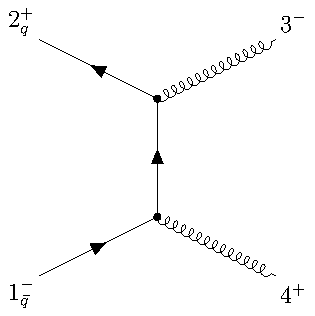
\includegraphics[scale=0.7]{chextra_solutions/figures/Atree_qbqgg_I.pdf}}}}
+ \underset{\textstyle\mathrm{(II)}}{\vcenter{\hbox{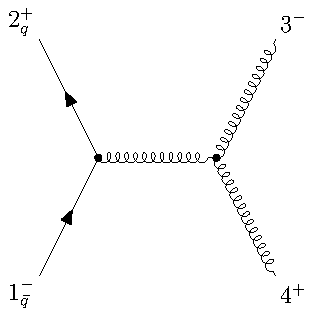
\includegraphics[scale=0.7]{chextra_solutions/figures/Atree_qbqgg_II.pdf}}}} \,.
\end{align}
The first graph (I) is proportional to
$[2| \slashed{\epsilon}_{3,-} (\slashed{p}_1+\slashed{p}_2) \slashed{\epsilon}_{4,+} |1\rangle\,,$
which vanishes for the reference-vector choice $\mu_{4}\, \tilde\mu_{4}=p_{1}$. This is so as
\begin{align}
\slashed{\epsilon}_{4,+} = - \frac{\sqrt{2}}{\vev{4 \mu_4}} \bigl(|4]\langle \mu_4| + | \mu_4 \rangle [4| \bigr) 
 \quad \Rightarrow \quad 
\slashed{\epsilon}_{4,+} |1\rangle = - \frac{\sqrt{2}}{\vev{4 \mu_4}} |4] \langle \mu_4 1 \rangle \stackrel{\mu_{4}=\la_{1}}{=}0 \,.
\end{align}
%
Evaluating the second graph (II) with the colour-ordered Feynman rules we obtain
%
\begin{align}
\label{graphII}
\text{(II)} = \frac{\i g^2}{2 q^2} [2|\gamma_{\mu}|1\rangle 
\Bigl [ \underbrace{ (\epsilon_{3,-}\cdot \epsilon_{4,+})\, p_{34}^{\mu}}_{(1)}
+ \underbrace{\epsilon_{4,+}^{\mu} \, (p_{4q}\cdot\epsilon_{3,-})}_{(2)} +
\underbrace{ \epsilon^{\mu}_{3,-}\, (p_{q3}\cdot
\epsilon_{4,+})}_{(3)}  \Bigr ]  \,,
\end{align}
%
where $q=p_1+p_2$ and $p_{ij} = p_i-p_j$.
The term $(2)$ vanishes for our choice $\mu_{4}\, \tilde\mu_{4}=p_{1}$,
\begin{align}
(2) \propto [2| \slashed{\epsilon}_{4,+} |1\rangle 
\stackrel{\mu_{4}\tilde\mu_{4}=p_{1}}{=} 0 \,.
\end{align}
For the term $(3)$, we note that $\slashed{\epsilon}_{3,-}
= \sqrt{2} \, (\, |3\rangle\, [\mu_{3}| + |\mu_{3}]\,\langle 3| \,)/[3\mu_{3}]$ 
to find
\begin{align}
(3) \propto
[2| \slashed{\epsilon}_{3}^{-}\, |1\rangle = \frac{\sqrt{2}}{[3\mu_{3}]}\,
\bev{2\mu_{3}}\, \vev{31}\,,
\end{align}
which is killed by the choice $\mu_3\tilde{\mu}_3 = p_2$.
Hence, for this choice of reference vectors only the term $(1)$ in \eqn{graphII} contributes. 
One has
\begin{align}
\epsilon_{3,-}\cdot\epsilon_{+,4}= - \frac{\vev{\mu_{4}3}\, \bev{\mu_{3}\,4}}{\vev{4\mu_{4}}
\, \bev{3\mu_{3}}}  \stackrel{\mu_{3}=\la_2, \mu_{4}=\la_1}{=}
-\frac{\vev{13}\, \bev{24}}{\vev{41}\, \bev{32}}\, ,
\end{align}
and, using momentum conservation,
\begin{align}
 [2|(\slashed{p}_{3}\, - \slashed{p}_{4}) |1\rangle = 2 \, \spB 23 \spA 31 \,.
\end{align}
Inserting these into the term $(1)$ of \eqn{graphII} and using $q^{2}=\vev{12}\bev{21}$ yields
\begin{align}
A^{\text{tree}}_{\bar q q gg}(1^-_{\bar{q}}, 2^+_q, 3^-, 4^+) &= - \i g^2 \frac{\vev{13}^{2}}{\vev{12}\vev{41}} \, \overbrace{\frac{\bev{24}\vev{43}}{\bev{21}\vev{43}}}^{-\bev{21}\vev{13}} = - \i g^2 \frac{\vev{13}^{3}\vev{23}}{\vev{12}\vev{23}\vev{34}\vev{41}}\,,
\end{align}
as claimed. 
%
The helicity count of our result is straightforward and correct:
\begin{align*}
&h_{1} [ A^{\text{tree}}_{\bar q q gg} ]=-\frac{1}{2}(3-1-1)=-\ft12 \,, \qquad
& h_{2}[A^{\text{tree}}_{\bar q q gg}]=-\ft12(1-1-1)=+\ft12\, , \\
& h_{3}[A^{\text{tree}}_{\bar q q gg} ]=-\ft12(4-1-1)=-1\, , \qquad
& h_{4}[A^{\text{tree}}_{\bar q q gg}]=-\ft12(0-1-1)=+1\,.
\end{align*}

%================================================

\section*{Exercise \ref{Exer:2.1}: The vanishing splitting function $\mathrm{Split}^{\mathrm{tree}}_+(x,a^+,b^+)$}
\label{Sol:2.1}
We parametrise the collinear limit $5^+ \parallel 6^+$ by
\begin{align}
\lambda_5 = \sqrt{x} \, \lambda_P \,, \qquad \tilde{\lambda}_5 = \sqrt{x} \, \tilde{\lambda}_P \,, \qquad 
\lambda_6 = \sqrt{1-x} \, \lambda_P \,, \qquad \tilde{\lambda}_5 = \sqrt{1-x} \, \tilde{\lambda}_P \,,
\end{align} 
with $P = \lambda_P \tilde{\lambda}_P = p_5 + p_6$. Substituting this into the Parke-Taylor formula~\eqref{ParkeTaylor1} for $A_{6}^{\rm tree}(1^{-}, 2^{-}, 3^{+}, 4^{+}, 5^{+}, 6^{+})$ gives
\begin{align}
A_{6}^{\rm tree}(1^{-}, 2^{-}, 3^{+}, 4^{+}, 5^{+}, 6^{+}) \stackrel{5 \parallel 6}{\longrightarrow} \frac{g}{\sqrt{x(1-x)}\,\vev{56}}\, \frac{\i g^3 \vev{12}^{4}}{\vev{12}\vev{23}\vev{34}\vev{4P}\vev{P1}} \,.
\end{align}
Comparing this to the expected collinear behaviour from \eqn{eq:collinear_limit},
\begin{align} \begin{aligned}
A_{6}^{\rm tree}(1^{-}, 2^{-}, 3^{+}, 4^{+}, 5^{+}, 6^{+}) \stackrel{5 \parallel 6}{\longrightarrow} \, & {\rm Split}_{-}^{\rm tree}(x,5^{+},6^{+})\, 
A_{5}^{\rm tree}(1^{-}, 2^{-}, 3^{+}, 4^{+}, P^{+}) \\ 
& + {\rm Split}_{+}^{\rm tree}(x,5^{+},6^{+}) \, A_{5}^{\rm tree}(1^{-}, 2^{-}, 3^{+}, 4^{+}, P^{-}) \,, 
\end{aligned} \end{align}
and using \eqn{ParkeTaylor1} for the $5$-gluon amplitudes, we see that the term with ${\rm Split}_{+}^{\rm tree}(x,5^{+},6^{+})$ is absent. Since $ A_{5}^{\rm tree}(1^{-}, 2^{-}, 3^{+}, 4^{+}, P^{-}) \neq 0$, we deduce that
\begin{align}
{\rm Split}_{+}^{\rm tree}(x,5^{+},6^{+}) = 0 \,,
\end{align} 
as claimed.

%================================================

\section*{Exercise \ref{Ex:2.2}: Soft functions in the spinor-helicity formalism}
\label{Sol:2.2}
%
The leading soft function for a positive-helicity gluon with colour-ordered neighbours $a$ and $b$ is given by eq.~\eqref{eq:S0explicit} with $n=a$ and $1=b$,
\begin{align} \label{eq:S0YMex1}
\mathcal{S}^{[0]}_{\text{YM}}\left(a,q^+,b\right) = \frac{g}{\sqrt{2}} \left(\frac{\epsilon_+ \cdot p_b}{p_b \cdot q} - \frac{\epsilon_+ \cdot p_a}{p_a \cdot q} \right)  \,.
\end{align}
Using \eqn{s1polarrel} for the polarisation vector with $\mu$ as reference spinor, we have that
\begin{align}
\frac{\epsilon_+ \cdot p_i}{p_i \cdot q} = \sqrt{2} \frac{\spA{\mu}{i}}{\spA{q}{i} \spA{\mu}{q}} \,.
\end{align}
Substituting this with $i=a,b$ into eq.~\eqref{eq:S0YMex1} and using the Schouten identity give
\begin{align}
\mathcal{S}^{[0]}_{\text{YM}}\left(a,q^+,b\right) =  g \, \frac{\spA ab}{\spA aq \spA qb} \,,
\end{align}
as claimed. We can obtain the negative-helicity soft function by acting with spacetime parity on the positive-helicity one. Parity exchanges $\lambda^{\alpha}$ and $\tilde{\lambda}^{\dot\alpha}$, which amounts to swapping $\spA ij$ with $\spB ji$.

We now turn to a positive-helicity graviton. The starting point is again eq.~\eqref{eq:S0explicit},
\begin{align} \label{eq:S0GMex1}
\mathcal{S}^{[0]}_{\text{GR}}\left(q^{++},1,\ldots,n\right) = \kappa \sum_{a=1}^n \frac{\epsilon^{++}_{\mu\nu} \, p_a^{\mu} p_a^{\nu}}{p_a \cdot q} \,.
\end{align}
We parametrise the graviton's polarisation vector by two copies of the gauge-field~one, 
\begin{align}
\epsilon_{++}^{\mu\nu}(q) = \epsilon_+^{\mu}(q,x) \, \epsilon_+^{\nu}(q,y) \,,
\end{align}
where we spelled out the arbitrary reference vectors $x$ and $y$. Substituting this into \eqn{eq:S0GMex1} and using \eqn{s1polarrel} for the polarisation vectors gives the desired result:
\begin{align}
\mathcal{S}^{[0]}_{\text{GR}}\left(q^{++},1,\ldots,n\right) = \kappa \sum_{a=1}^n \frac{\spA xa \spA ya \spB aq}{\spA xq \spA yq \spA aq} \,.
\end{align}
As above, the negative-helicity result can by obtained through parity conjugation.


%================================================
\newpage

\section*{Exercise \ref{Ex:qqggg}: A $\bar{q}qggg$ amplitude from collinear and soft limits}
\label{Sol:qqggg}
%
Let us consider the collinear limit $3^{-} \parallel 4^{+}$ of the quark-gluon amplitude \break
$A_{\bar{q}qggg}^{\text{tree}}(1_{\bar q}^{-}, 2_{q}^{+}, 3^{-}, 4^{+}, 5^{+})$. We parametrise the limit with
$$
\la_{3}\to \sqrt{x}\, \la_{P}\, , \quad  \la_{4}\to\sqrt{1-x}\, \la_{P} \,,
$$
where $P=p_3+p_4$. The collinear factorisation theorem implies that
\begin{align} \label{5qqlimit}
\begin{aligned}
A_{\bar{q}qggg}^{\text{tree}}(1_{\bar q}^{-}, 2_{q}^{+}, 3^{-}, 4^{+}, 5^{+})  
\stackrel{3 \parallel 4}{\longrightarrow} \, &
\text{Split}^{\text{tree}}_{+}(x,3^{-},4^{+})\, A_{\bar{q}qgg}^{\text{tree}}
(1_{\bar q}^{-}, 2_{q}^{+}, P^{-}, 5^{+}) \\ & +  
\text{Split}^{\text{tree}}_{-}(x,3^{-},4^{+})\, 
A_{\bar{q}qgg}^{\text{tree}}(1_{\bar q}^{-}, 2_{q}^{+}, P^{+}, 5^{+}) \\
= \, & \frac{g \, x^{2}}{\sqrt{x (1-x)}\, \vev{34}}\, \frac{- \i g^2 \vev{1P}^{3}\vev{2P}}{\vev{12}\vev{2P}\vev{P5}
\vev{51}} \,,
\end{aligned}
\end{align}
where we inserted \eqn{splittingfunctions} for the splitting functions, and eqs.~\eqref{eq:Aqqgg1} and~\eqref{eq:Aqqgg2} for the amplitudes.
The limiting form of \eqn{5qqlimit} suggests that the amplitude before the limit takes the~form
\begin{align}
A_{\bar{q}qggg}^{\text{tree}}(1_{\bar q}^{-}, 2_{q}^{+}, 3^{-}, 4^{+}, 5^{+}) = - \i g^3 \frac{\vev{13}^{3}\vev{23}}
{\vev{12}\vev{23}\vev{34}\vev{45}\vev{51}} \, .
\end{align}
The form above leads us to conjecture the following $n$-particle generalisation:
\be
A_{\bar{q}qg\ldots g}^{\text{tree}}(1_{\bar q}^{-}, 2_{q}^{+}, 3^{-}, 4^{+}, \ldots, n^{+}) = - \i g^{n-2} \frac{\vev{13}^{3}\vev{23}}
{\vev{12}\vev{23}\vev{34}\ldots\vev{n1}}\, .
\label{qqnpoint}
\ee
By analogy with eq.~\eqn{5qqlimit}, we see that the conjectured form of the $n$-particle amplitude~\eqn{qqnpoint} 
is consistent with the collinear limits $3^{-} \parallel 4^{+}$ and $i^{+} \parallel (i+1)^{+}$ for $i=4,\ldots , n-1$. 
Let us also study two soft limits.
First we take $\la_{3}\to 0$. Then we immediately see that
\begin{align}
A_{\bar{q}qg\ldots g}^{\text{tree}}(1_{\bar q}^{-}, 2_{q}^{+}, 3^{-}, 4^{+},\ldots, n^{+}) \stackrel{3^{-}\to 0}{\longrightarrow}  0 \,.
\end{align}
Since the expected behaviour in the limit is
\begin{align}
A_{\bar{q}qg\ldots g}^{\text{tree}}(1_{\bar q}^{-}, 2_{q}^{+}, 3^{-}, 4^{+},\ldots, n^{+})  \stackrel{3^{-}\to 0}{\longrightarrow} \mathcal{S}^{[0]}(2,3^{-},4)\,  
A_{\bar{q}qg\ldots g}^{\text{tree}}(1_{\bar q}^{-}, 2_{q}^{+}, 4^{+}, \ldots, n^{+}) \, ,
\end{align}
and the relevant soft function is not zero, this implies that 
\begin{align}
A_{\bar{q}qg\ldots g}^{\text{tree}}(1_{\bar q}^{-}, 2_{q}^{+}, 3^{+}, \ldots, n^{+}) = 0 \,,
\end{align}
which is thus the conjectured $n$-particle generalisation of \eqn{eq:Aqqgg1}. 
Taking the soft limit $4^{+}\to 0$ (or any other positive-helicity gluon leg) on the other hand again allows us to check the self-consistency of \eqn{qqnpoint},
\begin{align}
A_{\bar{q}qg\ldots g}^{\text{tree}}(1_{\bar q}^{-}, 2_{q}^{+}, 3^{-}, 4^{+}, \ldots, n^{+}) \stackrel{4^{+}\to 0}{\longrightarrow} 
\underbrace{g \frac{\vev{35}}{\vev{34}\vev{45}}}_{\mathcal{S}^{[0]}(3,4^{+},5)}\, A_{\bar{q}qg\ldots g}^{\text{tree}}(1_{\bar q}^{-}, 2_{q}^{+}, 3^{-}, 
5^{+}, \ldots, n^{+}) \, .
\end{align}

%================================================

\section*{Exercise \ref{Ex:6gNMHV}: The six-gluon split-helicity NMHV amplitude}
\label{Sol:6gNMHV}
%
We want to determine the NMHV six-gluon amplitude 
$A_{6}^{\text{tree}}(1^{+},2^{+},3^{+},4^{-},5^{-},6^{-})$. The $[6^-1^+\rangle$ shift leads to the BCFW recursion relation
%
\begin{align}
\begin{aligned}
& A_{6}^{\text{tree}}(1^{+}, 2^+, 3^+, 4^-, 5^-, 6^{-}) = \\
& \quad \sum_{i=3}^{5} \sum_{h=\pm} A_{i}^{\text{tree}}\left(\hat 1^+ , 2^+,\ldots , i-1, -{\hat P}^{-h}_{i}(z_{P_{i}})\right)\, 
\frac{\i}{P_{i}^{2}}
\, A_{8-i}^{\text{tree}}\left({\hat P}^{h}_{i}(z_{P_{i}}),i,\ldots , 5^-, \hat{6}^- \right)\,.
\end{aligned}
\end{align}
Since the all-plus/minus and single-plus/minus tree amplitudes vanish, only two contributions are non-zero. Diagrammatically, they are given by
\begin{align*}
\underset{\textstyle\mathrm{(I)}}{\vcenter{\hbox{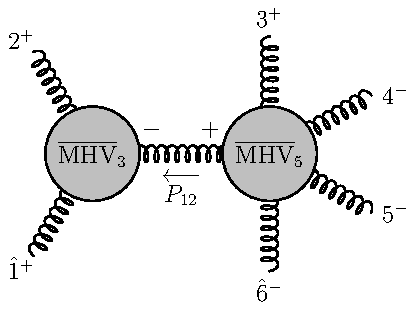
\includegraphics[scale=0.7]{chextra_solutions/figures/BCFW_6g_I.pdf}}}}
\quad \underset{\textstyle\mathrm{(II)}}{\vcenter{\hbox{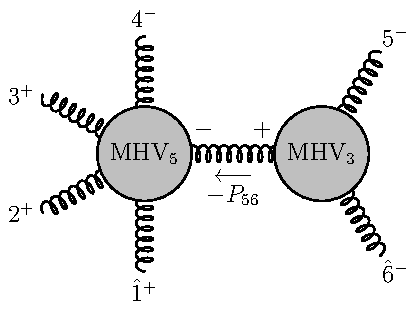
\includegraphics[scale=0.7]{chextra_solutions/figures/BCFW_6g_II.pdf}}}} 
\end{align*}
where we used the short-hand notation $P_{ij} = p_i+p_j$. The first diagram is given by
\begin{align}
\label{sh1}
\text{(I)} = \frac{- \i g \, \spB{\hat{1}}{2}^3}{\spB{2}{(-\hat P_{12})}\, \spB{(-\hat P_{12})}{\hat 1}}
\times \frac{\i}{\vev{12}\bev{21}} \times 
\frac{-\i g^3 \spB{\hat P_{12}}{3}^3}{\spB{3}{4}\,\spB{4}{5}\, \spB{5}{\hat{6}}\, \spB{\hat{6}}{ 
\hat P_{12}}} \, .
\end{align}
The corresponding $z$-pole is at $z_{\text{I}} = P_{12}^2/\spAB{6}{P_{12}}{1} = \spA 12 / \spA 62$. Hence we~have
\begin{align}
|\hat{1}\rangle = \frac{\spA{1}{6}}{\spA{6}{2}} |2\rangle \,, \quad |\hat 1] = |1] \,, \quad
|\hat{6}\rangle = |6\rangle \,, \quad |\hat{6}] = |6] + \frac{\spA{1}{2}}{\spA{6}{2}} |1] \,,
\end{align}
where we used the Schouten identity to simplify $|\hat{1}\rangle$, and, for $\hat{P}_{12} = \hat{p}_1 + p_2$,
\begin{align}
|\hat{P}_{12}\rangle = |2\rangle \,, \qquad  |\hat{P}_{12}] = |2] + \frac{\spA 61}{\spA 62} |1] \,.
\end{align}
By combining the above we obtain
\begin{align} \begin{aligned}
\bev{2 \hat{P}_{12}} &= \frac{\vev{61}}{\vev{62}}\, \bev{21}\, , \quad
\bev{\hat{P}_{12} \hat{1}} =\bev{21}\, , \quad  \bev{5\hat 6} = \frac{[5|P_{16}|2\rangle}{\spA 62}\, , \\
\bev{\hat{P}_{12} 3} &= \frac{\langle 6 | P_{12}|3]}{\vev{62}}\, , \quad
\bev{\hat 6 \hat{P}_{12}} = - \frac{P_{26}^{2}+P_{12}^{2}+P_{16}^{2}}{\vev{62}} \,.
\end{aligned} \end{align}
The expression for $\bev{\hat 6 \,\hat P_{12}}$ can be further simplified by noting that $P_{26}^{2}+P_{12}^{2}+P_{16}^{2} = (p_6+p_1+p_2)^2$.
Substituting all these into~\eqn{sh1}, with the sign convention~\eqref{negpspin}, gives our final expression for diagram (I):
\begin{align}
\text{(I)} = \i g^4 \frac{\spAB{6}{P_{12}}{3}^3}{\spA 61 \spA 12 \spB 34 \spB 45 \spBA{5}{P_{16}}{2}} \frac{1}{(p_6+p_1+p_2)^2}\,.
\end{align}
For the second diagram we start with
\begin{align} \label{eq:6gdiagII}
\text{(II)} =  \frac{\i g^3 \, \spA{4}{\hat P_{56}}^{3}}{\vev{\hat P_{56}\hat{1}}\vev{\hat{1}2}
\vev{23}\vev{34}}\times \frac{\i}{\vev{56}\bev{65}} \times \frac{\i g \, \vev{5\hat 6}^{3}}
{\vev{6 (-\hat{P}_{56})}\vev{(-\hat{P}_{56}) 5}} \,.
\end{align}
Now the shift parameter takes the value $z_{\text{II}} = \spB 65 / \spB 51$, which implies
\begin{align}
|\hat{1}\rangle = |1\rangle + \frac{\spB 56}{\spB 51} |6\rangle \,, \quad 
|\hat{6}\rangle = |6\rangle \,, \quad 
|\hat{P}_{56}\rangle = |5\rangle + \frac{\spB 16}{\spB 15} |6\rangle \,,
\end{align}
and hence
\begin{align} \begin{aligned}
\vev{4 \hat{P}_{56}} &= \frac{\langle 4 | P_{56}|1]}{\bev{51}}\, , \quad
\vev{\hat{P}_{56} \hat{1}} = \frac{(p_1+p_5+p_6)^2}{\bev{15}}\, ,\quad
\vev{5\hat{6}} = \vev{56}\, ,\\ 
\vev{6 \hat{P}_{56}}&= \vev{65}\, ,\quad
\vev{\hat{P}_{56} 5}= \frac{\bev{16}}{\bev{15}} \vev{65}\, , \quad
\vev{\hat{1}2}= \frac{[5|P_{16}|2\rangle}{\bev{51}}\, .
\end{aligned} \end{align}
Plugging these into \eqn{eq:6gdiagII} yields
\begin{align}
\text{(II)} = \i g^4 \frac{\spAB{4}{P_{56}}{1}^3}{ \vev{23} \vev{34} [16][65] \spBA{5}{P_{16}}{2} }  \frac{1}{(p_1+p_5+p_6)^2} \,.
\end{align}
Finally, by combining the two diagrams we obtain
\begin{align} \begin{aligned}
A_{6}^{\text{tree}}(1^{+},2^{+},3^{+}, {} & 4^{-},5^{-},6^{-}) = \i g^4 \biggl( \frac{\spAB{6}{P_{12}}{3}^3}{\spA 61 \spA 12 \spB 34 \spB 45 \spBA{5}{P_{16}}{2}} \frac{1}{(p_6+p_1+p_2)^2} \\
& + \frac{\spAB{4}{P_{56}}{1}^3}{ \vev{23} \vev{34} [16][65] \spBA{5}{P_{16}}{2} }  \frac{1}{(p_1+p_5+p_6)^2} \biggr) \,.
\end{aligned} \end{align}

%================================================

\section*{Exercise \ref{Ex:6gSoft}: Soft limit of the six-gluon split-helicity amplitude}
\label{Sol:6gSoft}
%
In the soft limit $p_5 \to 0$ we have the reduced momentum-conservation condition $p_{1}+p_{2}+p_{3}+p_{4}+p_{6}=0$, which implies that $(p_6+p_1+p_2)^2 = \spA 34 \spB 43$ and $(p_1+p_5+p_6)^2 = \spA 16 \spB 61$. Using these in \eqn{eq:A6NMHV} and pulling out the pole term $(\bev{45}\bev{56})^{-1}$ gives
%
\begin{align} 
\begin{aligned}
A_{6}^{\text{tree}}&(1^{+}, 2^{+}, 3^{+}, 4^{-}, 5^{-}, 6^{-}) \stackrel{5^- \to 0}{\longrightarrow}
\\ & \quad 
\frac{\i g^4}{[5|P_{16}|2\rangle\, \bev{45}\bev{56}} \biggl(
\frac{\langle 6|P_{12}|3]^{3} \bev{56}}{\vev{61}\vev{12}\bev{34}^2 \vev{43}}
+ \frac{ \langle 4|P_{56}|1]^{3} \bev{54} }{\vev{23}\vev{34} \bev{16}^2 \vev{61}}\,
\biggr) \,.
\end{aligned} 
\end{align}
%
We use the reduced momentum conservation and the Dirac equation to simplify
\begin{align}
\langle 6|P_{12}|3] & = - \langle 6|(p_3+p_4+p_6)|3] \nonumber \\
& = - \spA{6}{4} \spB{4}{3}\,,
\end{align}
and the soft limit for $\langle 4|P_{56}|1] = \spA{4}{6} \spB{6}{1}$, obtaining
%
\begin{align} 
\begin{aligned}
A_{6}^{\text{tree}}&(1^{+}, 2^{+}, 3^{+}, 4^{-}, 5^{-}, 6^{-}) \stackrel{5^- \to 0}{\longrightarrow}
\\ & \quad 
 \frac{\i g^4}{[5|P_{16}|2\rangle\, \bev{45}\bev{56}}\, \frac{\vev{46}^{3}}{\vev{12}\vev{23}\vev{34}
\vev{61}} \bigl(\bev{34}\bev{56} \vev{23} +  \bev{16}\bev{45}\vev{12} \bigr) \,.
\end{aligned} 
\end{align}
%
The two terms in the parentheses may be simplified using a Schouten identity~as
%
\begin{align}
 \overbrace{\bev{34}\bev{56}}^{-\bev{45}\bev{36}-\bev{53}\bev{46}} \hspace{-0.5cm} \vev{23}
 + \bev{16}\bev{45} \vev{12} & = \bev{54}[6|\overbrace{P_{13}}^{-p_{4}}|2\rangle + \bev{35}\bev{46}\vev{23} \nonumber \\
& = \bev{46}[5|P_{34}|2\rangle \nonumber \\
& = - \bev{46}[5|P_{16}|2\rangle\, .
\end{align}
%
By plugging this into the above we find
%
\begin{align}
A_{6}^{\text{tree}}(1^{+}, 2^{+}, 3^{+}, 4^{-}, 5^{-}, 6^{-})  &\stackrel{5^{-}\to 0}{\longrightarrow}
- g \frac{\bev{46}}{\bev{45}\bev{56}}  \times \frac{\i g^3 \, \vev{46}^{3}}{\vev{12}\vev{23}\vev{34}
\vev{61}}  \,,
\end{align}
%
which indeed matches the expected factorisation,
\begin{align}
A_{6}^{\text{tree}}(1^{+}, 2^{+}, 3^{+}, 4^{-}, 5^{-}, 6^{-})  &\stackrel{5^{-}\to 0}{\longrightarrow} \mathcal{S}^{[0]}_{\text{YM}}(4,5^{-},6) \times A_{5}^{\text{tree}}(1^{+}, 2^{+}, 3^{+}, 4^{-}, 6^{-})\,,
\end{align}
with the soft function given in \eqn{eq:SoftYM_minus}.


%================================================

\section*{Exercise \ref{Ex:2.helicity}: Mixed-helicity four-point scalar-gluon amplitude}
\label{Sol:2.helicity}
%
The $[4^- 1^+\rangle$ shift leads to the BCFW recursion
\begin{align} \begin{aligned}
A_{4}(1^{+},2_{\phi},3_{\bar\phi},4^{-}) & = \vcenter{\hbox{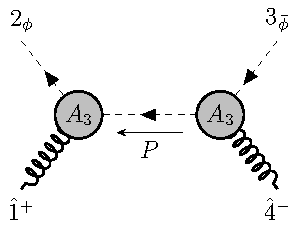
\includegraphics[scale=0.7]{chextra_solutions/figures/BCFW_massive_scalars.pdf}}} \\
& = A_{3}\left( (-\hat{P})_{\bar\phi}, \hat{1}^{+}, 2_{\phi} \right) \, \frac{\i}{P^2-m^2} \,
A_{3}\left(3_{\bar\phi},\hat{4}^{-}, \hat{P}_{\phi}\right) \\
& = \left( - \i \, \frac{ \spAB{r_1}{(-\hat{P})}{\hat{1}}}{\vev{r_1 \hat{1}}} \right) \frac{\i}{P^{2}-m^{2}} \left(-\i \,
\frac{\spAB{\hat{4}}{p_3}{r_4} }{\bev{\hat{4} r_4}} \right)
\,,
\end{aligned} \end{align}
where we used eqs.~\eqref{ssp} and~\eqref{ssm} for the three-point scalar-gluon amplitudes (with $g=1$), $P=p_1+p_2$, and $r_1$ ($r_4$) denotes the reference momentum of the gluon leg $1$ ($4$).
%
With the gauge choice $r_{1}=\hat{p}_4$ and $r_{4}=\hat{p}_1$ along with the identities
$|\hat 4\rangle=|4\rangle$ and $|\hat 1]=|1]$ for the $[4^- 1^+\rangle$ shift one has
%
\begin{align}
\vev{r_1 \hat{1}}&= \vev{41} \,, \quad 
\bev{\hat{4} \, r_4}= \bev{4 1} \,, \quad
\spAB{r_1}{\hat{P}}{\hat{1}} &= - \spAB{4}{p_3}{1} \,, \quad
\spAB{ \hat{4} }{p_3}{r_4}  &=  \spAB{4}{p_3}{1} \,.
\end{align}
%
Plugging these into the above yields the final compact result
\begin{align}
A_{4}(1^{+},2_{\phi},3_{\bar\phi},4^{-}) =  \i \,
\frac{\langle 4| p_{3}| 1]^{2}}{ (p_1+p_4)^2 \, [(p_1+p_2)^2-m^2] } \,.
\end{align}


%================================================

\section*{Exercise \ref{Ex:2.confalg}: Conformal algebra}
\label{Sol:2.confalg}
%
The commutation relations with the dilatation operator $d$,
\begin{align}
\left[d,p^{\a\da} \right]=p^{\a\da}\, , \quad \left[d,k_{\a\da} \right]=-k_{\a\da}\, , \quad 
\left[d,m_{\a\b} \right]=0=\left[d,{\overline m}_{\da\db}\right] \,,
\end{align}
are manifest from dimensional analysis. We recall in fact that $d$ measures the mass dimension, i.e.~$[d,f] = [f] f$ where $[f]$ denotes the dimension of $f$ in units of mass, and that the helicity spinors $\lambda_i$ and $\tilde{\lambda}_i$ have mass dimension $1/2$.
%
It remains for us to compute the commutator $[k_{\a\da}, p^{\b\db}]$, which is given by
%
\begin{align}
\left[k_{\a\da},p^{\b\db} \right] = 
\left[\partial_{\a},\la^{\b}\tla^{\db} \right]\, \partial_{\da}+ \partial_{\a} \left[ \partial_{\da}, \la^{\b}\tla^{\db} \right]
= \delta^{\b}_{\ \a}\, \tla^{\db}
\, \partial_{\da} + \delta^{\db}_{\ \da}\, \la^{\b}\partial_{\a}
+ \delta^{\b}_{\ \a}\, \delta^{\db}_{\da} \,.
\end{align}
By using \eqn{symlapa} for a single particle with raised index,
%
\begin{align}
\la^{\beta}\,\partial_{\alpha} = \epsilon^{\beta\rho} \, 
\la_{(\rho} \partial_{\alpha)}+ \frac{1}{2} \underbrace{\epsilon^{\beta\rho}\, \epsilon_{\rho\alpha}}_{=\, \delta^{\beta}_{\ \alpha}} \, \la^{\gamma}\partial_{\gamma} \,,
\end{align}
%
and the analogous equation with dotted indices, we obtain
%
\begin{align}
\left[k_{\a\da},p^{\b\db} \right] & = \delta^{\b}_{\ \a}\, \epsilon^{\db\dot\rho} \underbrace{\tilde{\la}_{(\dot{\rho}} \partial_{\dot{\alpha})}}_{ = \, \overline{m}_{\dot{\rho}\dot{\alpha}} }
+ \, \delta^{\db}_{\ \da}\, \epsilon^{\b\rho} \underbrace{\la_{(\rho} \partial_{\alpha)}}_{= \, m_{\rho \alpha}} + \, \delta^{\b}_{\ \a}\delta^{\db}_{\ \da}
 \Bigl( \underbrace{ \frac{1}{2} \la^{\gamma}\partial_{\gamma}+ \frac{1}{2}\tla^{\dot\gamma}\partial_{\dot\gamma}
+ 1}_{= \, d} \Bigr) \,,
\end{align}
%
which concludes the proof of \eqn{confalgebra}.




%================================================

\section*{Exercise \ref{Ex:2.invspecialconf}: Inversion and special conformal transformations}
\label{Sol:2.invspecialconf}
%
\noindent
a) Using the inversion transformation $I \, x^{\mu}= x^{\mu}/x^{2}$ and the translation
transformation $P^{\mu} \, x = x^{\mu }-a^{\mu}$ we 
have
%
\begin{align}
I \, P^{\mu} \, I \, x^{\mu}= I \, P^{\mu} \, \frac{x^{\mu}}{x^{2}} & =
 I \, \frac{x^{\mu}-a^{\mu}}{(x-a)^{2}} = 
\frac{\frac{x^{\mu}}{x^{2}}-a^{\mu}}{\left(\frac{x}{x^{2}}-a \right)^{2}}=
\frac{x^{\mu}-a^{\mu}x^{2}}{1-2 \, a\cdot x + a^{2}\, x^{2}} \,,
\end{align}
%
which equals the finite special conformal transformation in \eqn{finiteKaction}.
\medskip

\noindent
b) We begin by computing the Jacobian factor $|\partial x'/\partial x|$, i.e.\ the absolute value of the determinant of the matrix with entries $\partial x'^{\mu}/\partial x^{\nu}$ for $\mu,\nu=0,1,2,3$. It is convenient to decompose the special conformal transformation $x\to x'$ as in point~a):
\begin{align}
x^{\mu} \quad \overset{I}{\longrightarrow} \quad y^{\mu} \coloneqq \frac{x^{\mu}}{x^2} \quad \overset{P^{\mu}}{\longrightarrow} \quad z^{\mu} \coloneqq y^{\mu} - a^{\mu} 
\quad \overset{I}{\longrightarrow} \quad x'^{\mu} \coloneqq \frac{z^{\mu}}{z^2} \,.
\end{align}
The Jacobian factor for $x\to x'$ then factorises into the product of the Jacobian factors for the three separate transformations:
\begin{align}
\left| \frac{\partial x'}{\partial x} \right| = \left| \frac{\partial x'}{\partial z} \right| \, \left| \frac{\partial z}{\partial y} \right| \, \left| \frac{\partial y}{\partial x} \right| \,.
\end{align}
For the first inversion, $x^{\mu} \to y^{\mu}$, we have that
\begin{align}
\frac{\partial y^{\mu}}{\partial x^{\nu}} = \frac{1}{x^2}\left( \eta^{\mu}{}_{\nu} - 2 \, \frac{x^{\mu} x_{\nu}}{x^2} \right) \,,
\end{align}
so that the Jacobian factor takes the form
\begin{align}
\left| \frac{\partial y}{\partial x} \right| = \bigl(x^2\bigr)^{-4} \left| \mathrm{det}\left( \eta^{\mu}{}_{\nu} - 2 \, \frac{x^{\mu} x_{\nu}}{x^2} \right) \right| \,.
\end{align}
We use the representation of the determinant in terms of Levi-Civita symbols:
\begin{align}
\left| \frac{\partial y}{\partial x} \right| = \frac{\bigl(x^2\bigr)^{-4}}{4!} \left| 
  \epsilon_{\mu_1 \mu_2 \mu_3 \mu_4} \epsilon^{\nu_1 \nu_2 \nu_3 \nu_4}
  \left( \eta^{\mu_1}{}_{\nu_1} - 2 \, \frac{x^{\mu_1} x_{\nu_1}}{x^2} \right) \ldots  \left( \eta^{\mu_4}{}_{\nu_4} - 2 \, \frac{x^{\mu_4} x_{\nu_4}}{x^2} \right)  \right| \,.
\end{align}
The contractions involving two, one, or no factors of $\eta^{\mu_i}{}_{\nu_i}$ vanish because of the anti-symmetry of the Levi-Civita symbol.
The contractions with three factors of $\eta^{\mu_i}{}_{\nu_i}$ are equal. This leads us to
\begin{align}
\left| \frac{\partial y}{\partial x} \right| = \frac{\bigl(x^2\bigr)^{-4}}{4!} \left| 
  \epsilon_{\mu \nu \rho \sigma} \epsilon^{\mu \nu \rho \sigma} + 4 \, 
  \epsilon_{\mu \nu \rho \sigma_1} \epsilon^{\mu \nu \rho \sigma_2} \left( - 2 \, \frac{x^{\sigma_1} x_{\sigma_2}}{x^2} \right)
  \right| \,.
\end{align}
Using the identities $ \epsilon_{\mu \nu \rho \sigma} \epsilon^{\mu \nu \rho \sigma} = - 4!$ and $ \epsilon_{\mu \nu \rho \sigma_1} \epsilon^{\mu \nu \rho \sigma_2} = - 3! \, \eta^{\sigma_2}{}_{\sigma_1}$\footnote{We can derive this identity by tensor decomposition (see section~\ref{sec:TensorReduction}). We write $ \epsilon_{\mu \nu \rho \sigma_1} \epsilon^{\mu \nu \rho \sigma_2} = c \, \eta^{\sigma_2}{}_{\sigma_1}$, and fix $c=-3!$ by contracting both sides by $\eta^{\sigma_1}{}_{\sigma_2}$ and solving for $c$.} gives
\begin{align}
\left| \frac{\partial y}{\partial x} \right| = \bigl(x^2\bigr)^{-4}  \,.
\end{align}
Similarly, for the second inversion, $z \to x'$, we have 
\begin{align} \begin{aligned}
\left| \frac{\partial x'}{\partial z} \right| & = \bigl(z^2\bigr)^{-4}  \\
& = \left( \frac{1 - 2 \, a \cdot x + a^2 x^2}{x^2} \right)^{-4} \,.
\end{aligned} \end{align}
The Jacobian factor of the translation $y^{\mu} \to z^{\mu} = y^{\mu}-a^{\mu}$ is simply $1$, as the translation parameter $a^{\mu}$ does not depend on $y^{\mu}$. Putting the above together gives
\begin{align}
\left| \frac{\partial x'}{\partial x} \right| =  \left(1 - 2 \, a \cdot x + a^2 x^2\right)^{-4} \,.
\end{align}

\noindent
We now consider the transformation rule for the scalar field $\Phi$ in \eqn{eq:conformal_scalar},
\begin{align} \label{eq:conformal_scalar_2}
\Phi^{\prime}(x^{\prime}) =  \left(1 - 2 \, a \cdot x + a^2 x^2\right)^{\Delta} \Phi(x) \,,
\end{align}
and expand both sides in a Taylor series around $a^{\mu} = 0$. For the LHS we obtain
\begin{align} \label{eq:fprimeTaylor} \begin{aligned}
\Phi^{\prime}\left( x^{\prime} \right) & = \Phi^{\prime}(x) + a^{\mu} \left( \frac{\partial x^{\prime \, \nu}}{\partial a^{\mu}} \right) \biggl|_{a=0} \partial_{\nu} \Phi^{\prime}(x) + \mathcal{O}\bigl(a^2\bigr) \\
& = \Phi^{\prime}(x) + a^{\mu} \left( - \eta_{\mu}{}^{\nu} x^2 + 2 \, x_{\mu} \, x^{\nu} \right) \partial_{\nu} \Phi^{\prime}(x) + \mathcal{O}\bigl(a^2\bigr) \,.
\end{aligned} \end{align}
Since $\Phi^{\prime}(x) - \Phi(x) = \mathcal{O}(a)$, we can replace $\partial_{\nu} \Phi^{\prime}(x) $ by $\partial_{\nu} \Phi(x) $ in the above. Plugging this into \eqn{eq:conformal_scalar_2} and expanding also the RHS gives
\begin{align}
 \Phi^{\prime}(x) + a^{\mu} \left( - \eta_{\mu}{}^{\nu} x^2 + 2 \, x_{\mu} \, x^{\nu} \right) \partial_{\nu} \Phi^{\prime}(x)  = \Phi(x) - 2 \, \Delta \, (a \cdot x) \, \Phi(x) + \mathcal{O}\bigl(a^2\bigr) \,.
\end{align}
By comparing this to the defining equation of the generators~\eqref{eq:fxprime},
\begin{align}
\Phi^{\prime}\left( x \right ) = \left[ 1 - \i \, a^{\mu} \, K_{\mu} +  \mathcal{O}\bigl(a^2\bigr) \right] \, \Phi(x) \,,
\end{align}
we can read off the explicit form of the generator,
\begin{align}
K_{\mu} = \i \left[ x^2 \, \partial_{\mu} - 2 \, x_{\mu} \left( x^{\nu} \partial_{\nu} + \Delta \right) \right] \,,
\end{align}
as claimed.





%================================================

\section*{Exercise \ref{Ex:2.kin_Jacobi}: Kinematical Jacobi identity}
\label{Sol:2.kin_Jacobi}
We start from the expression of $n_s$ given in eq.~\eqref{ns}.
We choose the reference momenta $r_i$ for the polarisation vectors $\epsilon_i$ so as to kill as many terms as possible. We recall that $\epsilon_i \cdot r_i = 0$. Choosing $r_1 = p_2$, $r_2 = p_1$, $r_3 = p_4$, and $r_4 = p_3$ yields
\begin{align}
\begin{aligned}
n_{s}= \phantom{ } & (p_1 \cdot p_2) \left[ (\epsilon_1\cdot \epsilon_2) (\epsilon_3\cdot \epsilon_4)   
  - (\epsilon_1\cdot \epsilon_3) (\epsilon_2\cdot \epsilon_4) 
  + (\epsilon_2\cdot \epsilon_3) (\epsilon_1\cdot \epsilon_4) \right] \\
  & + 2 \, (p_2 \cdot p_3)  (\epsilon_1\cdot \epsilon_2) (\epsilon_3\cdot \epsilon_4) \,.
\end{aligned}
\end{align}
The other factors are obtained from $n_s$ by replacing the particles' labels as
\begin{align}
n_t = n_s \bigl|_{1 \to 2, 2 \to 3, 3 \to 1} \,, \qquad \qquad n_u = n_s \bigl|_{1 \to 3, 2 \to 1, 3 \to 2} \,.
\end{align}
Adding the three factors gives
\begin{align}
\begin{aligned}
n_s + n_t + n_u = \phantom{ } & \bigl[ (\epsilon_1 \cdot \epsilon_4) (\epsilon_2 \cdot \epsilon_3) + 
  (\epsilon_1 \cdot \epsilon_3) (\epsilon_2 \cdot \epsilon_4) + (\epsilon_1 \cdot \epsilon_2) (\epsilon_3 \cdot \epsilon_4) \bigr]  \\
 & \times   ( p_1 \cdot p_2 +  p_2 \cdot p_3 + p_3 \cdot p_1 ) \,,
\end{aligned}
\end{align}
which vanishes because of momentum conservation.

%================================================

\section*{Exercise \ref{Ex:2.KLT}: Five-point KLT relation}
\label{Sol:2.KLT}
%
The squaring relation~\eqref{eq:MtoA2} in the five-point case reads
\begin{align}  \label{eq:MtoA2_5pt}
M_{5}^{\text{tree}}(1,2,3,4,5) = \sum_{\sigma,\rho\in S_{2}} A_{5}^{\text{tree}}(1,\sigma,4,5)
\, S[\sigma|\rho] \, A_{5}^{\text{tree}}(1,\rho,5,4) \,,
\end{align}
where $S_2$ is the set of permutations of $\{2,3\}$, namely $S_2 = \bigr\{ \{2,3\}, \, \{3,2\} \bigl\}$. 
We recall that the KLT kernels $S[\sigma|\rho]$ are given by \eqn{KLTkernel} with $n=5$,
\begin{align}
S[\sigma|\rho] = \prod_{i=2}^{3} \biggl[ 
2 \, p_{1}\cdot p_{\sigma_{i}} + \sum_{j=2}^{i} 2 \, p_{\sigma_{i}}\cdot p_{\sigma_{j}}\, \theta(\sigma_{j},
\sigma_{i})_{\rho}
\biggr] \,,
\end{align}
where $\theta(\sigma_{j}, \sigma_{i})_{\rho}=1$ if $\sigma_{j}$ is before $\sigma_{i}$ in the permutation $\rho$,
and zero otherwise. We then have
\begin{align} \begin{aligned}
S\left[(2,3)|(2,3)\right] & = 2 \, p_1 \cdot p_2 \, \bigl[ 2 \, p_1 \cdot p_3 + 2 \, p_3 \cdot p_2 \, \overbrace{\theta(2,3)_{(2,3)}}^{= \, 1} \bigr] \\
& = s_{12} ( s_{13} + s_{23} ) \,,
\end{aligned} \end{align}
where $s_{ij} = 2 \, p_i \cdot p_j$, and similarly
\begin{align} \begin{aligned}
& S\left[(3,2)|(2,3)\right] = s_{12} \, s_{13} = S\left[(2,3)|(3,2)\right]  \,, \\ 
& S\left[(3,2)|(3,2)\right] = s_{13} (s_{12}+s_{23}) \,.
\end{aligned} \end{align}
Plugging the above into the squaring relation~\eqref{eq:MtoA2_5pt} gives
\begin{align} \label{eq:M5KLT1} \begin{aligned}
& M_{5}^{\text{tree}}(1,2,3,4,5) = \\
 & \quad s_{12} A_5^{\text{tree}}(1,2,3,4,5) \bigl[ s_{13} A^{\text{tree}}_5(1,3,2,5,4) + (s_{13}+s_{23}) A^{\text{tree}}_5(1,2,3,5,4) \bigr]  \\
 & \quad + s_{13} A_5^{\text{tree}}(1,3,2,4,5) \bigl[ s_{12} A_5^{\text{tree}}(1,2,3,5,4) + (s_{12}+s_{23}) A_5^{\text{tree}}(1,3,2,5,4) \bigr] \,.
\end{aligned} \end{align}
The terms in the square brackets can be simplified using the BCJ relations~\eqref{eq:BCJn}. For instance, for the first term we use
\begin{align} \begin{aligned}
& p_3 \cdot p_1 \, A^{\text{tree}}_5(1,3,2,5,4) + p_3 \cdot (p_1+p_2) \, A^{\text{tree}}_5(1,2,3,5,4) \\
& +  p_3 \cdot (p_1+p_2+p_5) \, A^{\text{tree}}_5(1,2,5,3,4) = 0 \,,
\end{aligned} \end{align}
which is obtained by replacing $1\to 3$, $2\to 1$, $3\to 2$, $4 \to 5$ and $5 \to 4$ in \eqn{eq:BCJn} with $n=5$. Substituting
\begin{align} \begin{aligned}
s_{13} \, A^{\text{tree}}_5(1,3,2,5,4) + (s_{13}+s_{23}) \, A^{\text{tree}}_5(1,2,3,5,4)  = s_{34} \, A^{\text{tree}}_5(1,2,5,3,4) \,, \\
s_{12} \, A_5^{\text{tree}}(1,2,3,5,4) + (s_{12}+s_{23}) \, A_5^{\text{tree}}(1,3,2,5,4) =  s_{24} \, A_5^{\text{tree}}(1,3,5,2,4) \,,
\end{aligned} \end{align}
into \eqn{eq:M5KLT1} finally gives
\begin{align} \begin{aligned}
M_{5}^{\text{tree}}(1,2,3,4,5) & = s_{12} \, s_{34} \, A_5^{\text{tree}}(1,2,3,4,5) \, A^{\text{tree}}_5(1,2,5,3,4) \\
 & \phantom{{} =} + s_{13} \, s_{24} \, A_5^{\text{tree}}(1,3,2,4,5) \, A_5^{\text{tree}}(1,3,5,2,4) \,,
\end{aligned} \end{align}
as claimed.

%================================================

\section*{Exercise \ref{Ex:3.1}: The four-gluon amplitude in $\mathcal{N}=4$ super-symmetric Yang-Mills theory}
\label{Sol:3.1}
%
We begin with the $s_{12}$ channel. The cut integrand is given by the following product of tree amplitudes:
\begin{align}
\mathcal{C}^{\mathcal{N}=4}_{12|34} & \coloneqq \mathcal{C}_{12|34}\left(I^{(1)}_{\mathcal{N}=4}(1^-,2^-,3^+,4^+) \right) \nonumber \\
& \phantom{:} =  \sum_{h_1,h_2} \i \, A^{(0)}\left( (-l_1)^{-h_1},1^-,2^-,(l_2)^{h_2} \right) \, \i \, A^{(0)}\left( (-l_2)^{-h_2},3^+,4^+,(l_1)^{h_1} \right) \nonumber \\
& \phantom{\coloneqq {}} - 4 \, \sum_{h_1,h_2} A^{(0)}\left( (-l_1)^{-h_1}_{\Lambda},1^-,2^-,(l_2)^{h_2}_{\Lambda} \right) \, A^{(0)}\left( (-l_2)^{-h_2}_{\Lambda},3^+,4^+,(l_1)^{h_1}_{\Lambda} \right) \nonumber \\
& \phantom{\coloneqq {}} + 6 \, \i \, A^{(0)}\left( (-l_1)_{\phi},1^-,2^-,(l_2)_{\phi} \right) \, \i \, A^{(0)}\left( (-l_2)_{\phi},3^+,4^+,(l_1)_{\phi} \right) \,.
\end{align}
The constant factors multiplying the amplitudes deserve a few remarks. First, we have a factor counting each field's multiplicity in the $\mathcal{N}=4$ super-multiplet: $1$ gluon ($g$), $4$ gluinos ($\Lambda$), and $6$ scalars ($\phi$). Next, the factors of imaginary unit ``$\i$'' follow from the factorisation properties of tree-level amplitudes as discussed below \eqn{eq:multiparticlepole}. In particular, note that the factorisation of the fermion line does not require any factors of ``$\i$'', as opposed to gluons and scalars. Finally, the gluino's contribution comes with a further factor of $-1$ coming from the Feynman rule for the closed fermion loop. The only non-vanishing contribution comes from the product of purely gluonic amplitudes with $h_1=-$ and $h_2=+$,
\begin{align}
\mathcal{C}_{12|34}^{\mathcal{N}=4} = 
  \i \, A^{(0)}\left( (-l_1)^{+},1^-,2^-,(l_2)^{+} \right) \, \i \,
  A^{(0)}\left( (-l_2)^{-},3^+,4^+ ,(l_1)^{-} \right) \,.
\end{align}
This is the same as in the non-supersymmetric YM theory computed in section~\ref{sec:3.2} (see \eqn{eq:C12|34YM}), hence we can immediately see that 
\begin{align}
\mathcal{C}_{12|34}\left( I^{(1)}_{\mathcal{N}=4}(1^-,2^-,3^+,4^+) \right)=\mathcal{C}_{12|34}\left( I^{(1)}(1^-,2^-,3^+,4^+) \right) \,, 
\end{align}
as claimed.

In contrast to the $s_{12}$ channel, all fields contribute to the $s_{23}$-channel cut:
\begin{align}
\begin{aligned}
\mathcal{C}_{23|41}^{\mathcal{N}=4} & \coloneqq \mathcal{C}_{23|41}\left(I^{(1)}_{\mathcal{N}=4}(1^-,2^-,3^+,4^+) \right)  \\
& \phantom{:} =  \i \, A^{(0)}\left( (-l_1)^{+},2^-,3^+,(l_2)^{-} \right)
  \, \i \, A^{(0)}\left( (-l_2)^{+},4^+,1^-,(l_1)^{-} \right) \\
  %
  & \phantom{{} \coloneqq}  + \i \, A^{(0)}\left( (-l_1)^{-},2^-,3^+,(l_2)^{+} \right)
  \, \i \, A^{(0)}\left( (-l_2)^{-},4^+,1^-,(l_1)^{+} \right) \\
  %
  &  \phantom{{} \coloneqq}  - 4 \, A^{(0)}\left( (-l_1)^{-}_{\Lambda},2^-,3^+,(l_2)^{+}_{\Lambda} \right) \,
  A^{(0)}\left( (-l_2)^{-}_{\Lambda},4^+,1^-,(l_1)^{+}_{\Lambda} \right) \\ 
  %
  &  \phantom{{} \coloneqq}  - 4 \, A^{(0)}\left( (-l_1)^{+}_{\Lambda},2^-,3^+,(l_2)^{-}_{\Lambda} \right) \,
  A^{(0)}\left( (-l_2)^{+}_{\Lambda},4^+,1^-,(l_1)^{-}_{\Lambda} \right) \\ 
  %
  &  \phantom{{} \coloneqq}  + 6 \, \i \, A^{(0)}\left( (-l_1)_{\phi},2^-,3^+,(l_2)_{\phi} \right) \, \i \,
  A^{(0)}\left( (-l_2)_{\phi},4^+,1^-,(l_1)_{\phi} \right) \,.
\end{aligned}
\end{align}
The second and fourth terms can be obtained by swapping $1 \leftrightarrow 2$ and $3 \leftrightarrow 4$ in the first and the third ones, respectively. We put all terms over a common denominator:
\begin{align}
{\rm D} = \langle 1 l_1 \rangle \langle l_1 l_2 \rangle \langle l_2 4 \rangle \langle 4 1 \rangle \langle l_1 2 \rangle \langle 23 \rangle \langle 3 l_2 \rangle \langle l_2 l_1 \rangle \,.
\end{align}
Factoring it out we have
\begin{align}
\begin{aligned}
{\rm D} \, \mathcal{C}_{23|41}^{\mathcal{N}=4} = \ & \spA 1{l_1}^4  \spA 2{l_2}^4 + \spA 2{l_1}^4 \spA 1{l_2}^4 - 4 \, \spA {l_1}1 \spA{l_1}2^3 \spA{l_2}2 \spA{l_2}1^3 \\
 & - 4 \, \spA {l_1}2 \spA{l_1}1^3 \spA{l_2}1 \spA{l_2}2^3   + 6 \, \spA {l_1}1^2  \spA {l_2}1^2  \spA {l_1}2^2  \spA {l_2}2^2\,.
\end{aligned}
\end{align}
Here the ``magic'' of $\mathcal{N}=4$ super Yang-Mills theory comes into play: the five terms above conspire together to form the fourth power of a binomial, 
\begin{align}
\mathcal{C}_{23|41}^{\mathcal{N}=4} = \frac{\bigl(\spA 1{l_2} \spA 2 {l_1} - \spA 1{l_1} \spA 2{l_2}\bigr)^4}{{\rm D}} \,,
\end{align}
which can be further simplified using a Schouten identity, obtaining
\begin{align}
\mathcal{C}_{23|41}^{\mathcal{N}=4} &  = \frac{ \spA {l_1}{l_2}^4 \spA 12^4}{{\rm D}} \nonumber \\
& = \frac{  \spA {l_1}{l_2}^2 \spA 12^4}{\spA {l_1}1 \spA {l_1} 2 \spA {l_2}3 \spA {l_2}4 \spA 23 \spA 14} \,.
\end{align}
This matches $\mathcal{C}_{23|41}^{\text{box}}$ (see \eqn{eq:tchannelcut2}), and we can thus conclude that
\begin{align}
\mathcal{C}_{23|41}\left( I^{(1)}_{\mathcal{N}=4}(1^-,2^-,3^+,4^+) \right) =\mathcal{C}_{23|41}^{\text{box}}\left( I^{(1)}(1^-,2^-,3^+,4^+) \right) \,.
\end{align}


%================================================

\section*{Exercise \ref{Ex:3.2}: Quadruple cuts of five-gluon MHV scattering amplitudes}
\label{Sol:3.2}
%
\begin{enumerate}[a)]
\item We parametrise the loop momentum $l_1$ using the spinors of the external momenta as in \eqn{eq:quadcutmombasis}. We then rewrite the quadruple cut equations,
\begin{align}
\begin{cases} l_1^2 = 0 \,, \\
l_2^2 = (l_1-p_2)^2 = 0  \,, \\
l_3^2 = (l_1-p_2-p_3)^2 = 0 \,, \\
l_4^2 = (l_1+p_1)^2 = 0 \,,
\end{cases}
\end{align}
in terms of the parameters $\alpha_i$, as
\begin{align}
\begin{cases} \alpha_1 s_{12} = 0 \,, \\
\alpha_2 s_{12} = 0 \,, \\
(\alpha_1 \alpha_2-\alpha_3 \alpha_4)s_{12} = 0 \,, \\
\alpha_1 s_{13} + \alpha_2 s_{23} + \alpha_3 \spA13 \spB32 + \alpha_4 \spA23 \spB31 = s_{23} \,.
\end{cases}
\end{align}
For generic kinematics this system has two solutions:
\begin{align}
\left(l_1^{(1)}\right)^{\mu} = \frac{\spA 23}{\spA 13} \frac{1}{2} \langle 1 | \gamma^{\mu} | 2 ] \,, \qquad 
\left(l_1^{(2)}\right)^{\mu} = \frac{\spB 23}{\spB 13} \frac{1}{2} \langle 2 | \gamma^{\mu} | 1 ] \,.
\end{align}
The spinors of the on-shell loop momenta on the first solution can be chosen as
\begin{align} \label{eq:l1solSpinors}
\begin{alignedat}{2}
 & |l_1^{(1)} \r> =  \frac{\spA23}{\spA13} |1\r> \,, \qquad \quad && |l_1^{(1)}] = |2] \,, \\
 & |l_2^{(1)} \r> = \frac{\spA21}{\spA13} |3\r> \,, && |l_2^{(1)}] = |2] \,, \\
 & |l_3^{(1)} \r> = |3\r>  \,, && |l_3^{(1)}] = \frac{\spA21}{\spA13} |2] - |3] \,, \\
 & |l_4^{(1)} \r> = |1\r> \,, && |l_4^{(1)}] = |1] + \frac{\spA23}{\spA13} |2] \,.
\end{alignedat}
\end{align}
The spinors for the second solution, $l_1^{(2)}$, are obtained by swapping $\langle \rangle \leftrightarrow []$ in the first one.
%
For each solution $l_1^{(s)}$, the quadruple cut is is obtained by summing over all internal helicity configurations $\vec h = (h_1,h_2,h_3,h_4)$ (with $h_i = \pm$) the product of four tree-level amplitudes, 
 \begin{equation}
    \mathcal{C}_{1|2|3|45}\left( I^{(1)}(1^-,2^-,3^+,4^+,5^+) \right) \Bigl|_{l_1^{(s)}} = \sum_{\vec{h}} 
    \raisebox{-2cm}{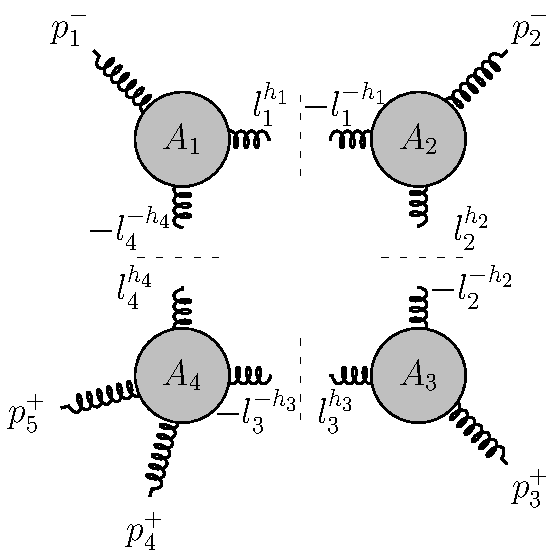
\includegraphics[width=4.3cm]{chextra_solutions/figures/5g_1l_1c2c3c45_generic.pdf}} \Biggl|_{l_1^{(s)}} \,.
    \label{eq:quadcut1_5g_generic}
  \end{equation}
%
Consider $A_4$. The only non-vanishing four-gluon tree-level amplitude with two positive-helicity gluons is the MHV one, namely $h_4=-h_3=-$. $A_3$ is thus $\overline{\text{MHV}}$, and $h_2=+$. Since MHV/$\overline{\text{MHV}}$ three-point vertices cannot be adjacent, $A_2$ must be MHV, and $A_1$ $\overline{\text{MHV}}$. This fixes the remaining helicity, $h_1=+$. The quadruple cuts therefore receive contribution from one helicity configuration only, which we represent using the black/white notation as
  \begin{equation}
    \mathcal{C}_{1|2|3|45}\left( I^{(1)}(1^-,2^-,3^+,4^+,5^+) \right)  = 
    \raisebox{-2cm}{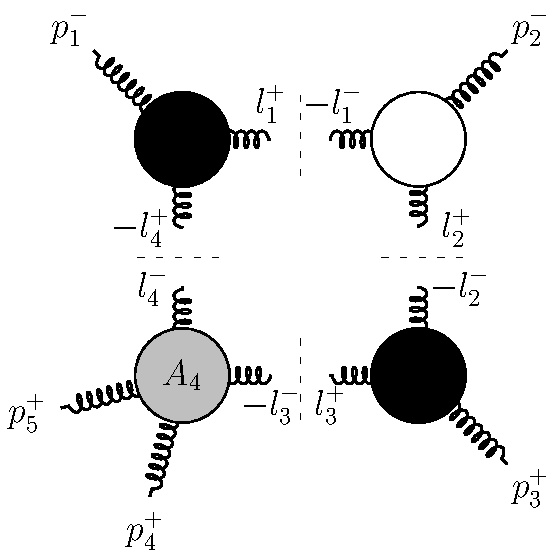
\includegraphics[width=4.3cm]{chextra_solutions/figures/5g_1l_1c2c3c45_blackwhite.pdf}}   \,.
    \label{eq:quadcut1_5g_generic}
  \end{equation}
Recall that the trivalent vertices impose constraints on the momenta. The $\overline{\text{MHV}}$ vertex attached to $p_1$ and the MHV vertex attached to $p_2$ imply that $|l_1\rangle \propto |1\rangle$ and $|l_1] \propto |2]$, or equivalently that $l_1^{\mu} \propto \langle 1 | \gamma^{\mu} |2]$.
Only the solution $l_1^{(1)}$ is compatible with this constraint. Indeed, we can show explicitly that the contribution from the second solution vanishes, for instance
\begin{align}
\vcenter{\hbox{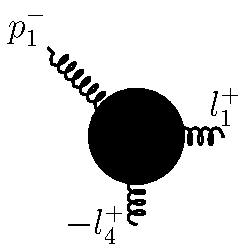
\includegraphics[width=2.2cm]{chextra_solutions/figures/MHVb_3pt_vanishing.pdf}}} \Biggl|_{l_1^{(2)}} 
= \frac{[l_1 (-l_4)]^3}{[l_1(-l_4)] [(-l_4)1]} \biggr|_{l_1^{(2)}} = 0 \,,
\end{align}
where we used $|l_1^{(2)}] = \bigl([23]/[13] \bigr) |1]$ and $|l_4^{(2)}] = |1]$. We assign spinors to $-p$ according to the convention~\eqref{negpspin}, namely $|-p\rangle = \i |p\rangle$ and $|-p] = \i |p]$. We thus have that
\begin{align}
 \mathcal{C}_{1|2|3|45}\left( I^{(1)}(1^-,2^-,3^+,4^+,5^+) \right) \biggl|_{l_1^{(2)}}  = 0 \,.
\end{align}
%
On the first solution, the quadruple cut is given by
\begin{align}
 \mathcal{C}_{1|2|3|45} \bigl|_{l_1^{(1)}}  = 
\frac{\spB {l_1}{l_4}^3}{\spB 1{l_1} \spB {l_4}1} \frac{\spA{l_1}2^3}{\spA2 {l_2} \spA{l_2}{l_1}}
  \frac{\spB 3{l_3}^3}{\spB{l_3}{l_2} \spB{l_2}3} \frac{\spA {l_4}{l_3}^3}{\spA{l_3}4 \spA45 \spA 5{l_4} } \Biggl|_{l_1^{(1)}} \,,
\end{align}
where we omitted the argument of $\mathcal{C}$ for the sake of compactness. Plugging in the spinors from \eqn{eq:l1solSpinors} and simplifying gives
\begin{align}
 \mathcal{C}_{1|2|3|45}\left( I^{(1)}(1^-,2^-,3^+,4^+,5^+) \right) \biggl|_{l_1^{(1)}}  = \i \, s_{12} s_{34} \left( \frac{\i \, \spA12^3}{\spA23 \spA34 \spA45 \spA51} \right) \,,
\end{align}
where in the parentheses we recognise the tree-level amplitude. Averaging over the two cut solutions 
(as in \eqn{eq:4gquadcutfinal} for the four-gluon case) gives the four-dimensional coefficient of the scalar box integral,
\begin{align}
c_{0;1|2|3|45}(1^-,2^-,3^+,4^+,5^+)  & = \frac{1}{2} \sum_{s=1}^2  \mathcal{C}_{1|2|3|45}\left( I^{(1)}(1^-,2^-,3^+,4^+,5^+) \right) \biggl|_{l_1^{(s)}} \nonumber \\
& = \frac{\i}{2} s_{12} s_{34} A^{(0)}(1^-,2^-,3^+,4^+,5^+) \,,
\end{align}
as claimed.

\smallskip

\item The solution of the quadruple cut can be obtained as in part a) of this exercise. Alternatively, we can take a more direct route by exploiting the black/white formalism for the trivalent vertices.
On each of the two solutions $l_1^{(s)}$ the quadruple cut is given by
\begin{align}
 \mathcal{C}_{1|23|4|5} \left( I^{(1)}(1^+,2^+,3^-,4^+,5^-)  \right) \Bigl|_{l_1^{(s)}} = \sum_{\vec{h}} \vcenter{\hbox{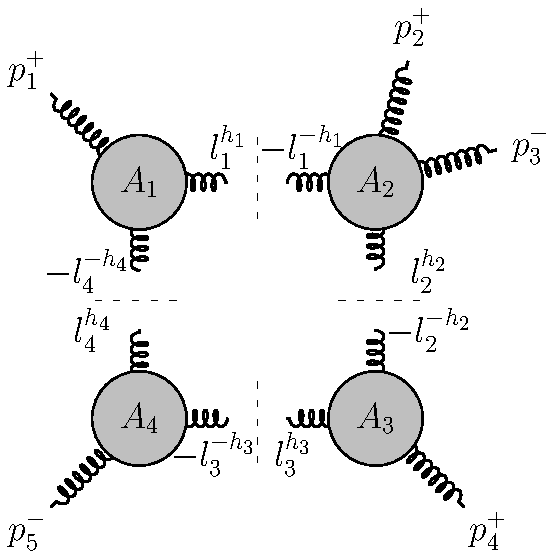
\includegraphics[width=4.3cm]{chextra_solutions/figures/5g_1l_1c23c4c5_generic.pdf}}} \Biggl|_{l_1^{(s)}}\,.
\end{align}
The only non-vanishing tree-level four-point amplitude is the MHV (or equivalently $\overline{\text{MHV}}$) one, so we have either $h_1=h_2=-$ or $h_1=h_2=+$. Specifying $h_1$ and $h_2$ and excluding adjacent black/white vertices fixes all the other helicities, so that the quadruple cut receives contribution from two helicity configurations:
%
\begin{align}
 \mathcal{C}_{1|23|4|5}^{(a)} = \hspace{-0.3cm} \vcenter{\hbox{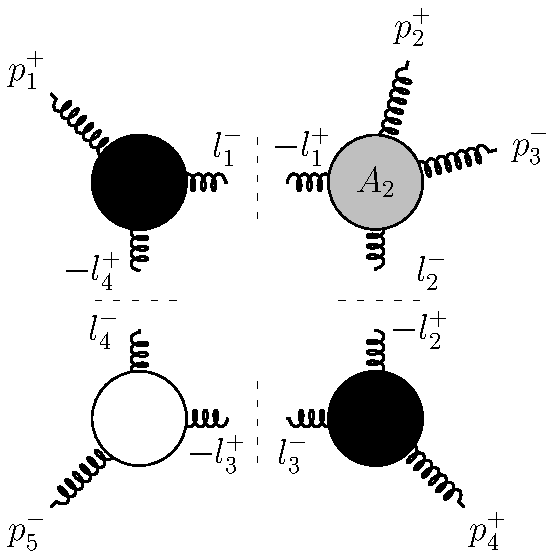
\includegraphics[width=4.3cm]{chextra_solutions/figures/5g_1l_1c23c4c5_BW1.pdf}}} \hspace{-0.3cm} \,,
\ \
 \mathcal{C}_{1|23|4|5}^{(b)} = \hspace{-0.3cm} \vcenter{\hbox{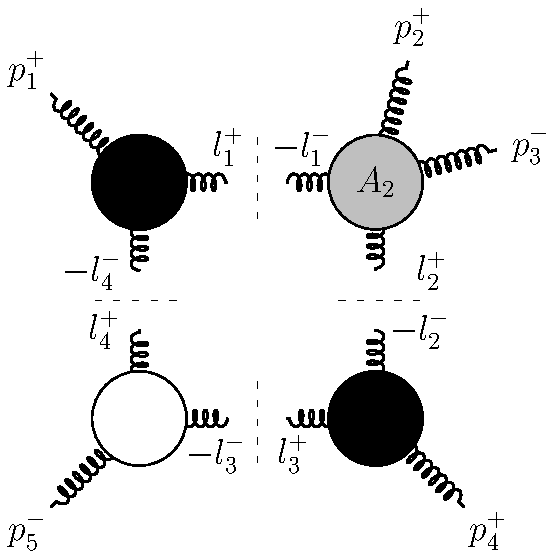
\includegraphics[width=4.3cm]{chextra_solutions/figures/5g_1l_1c23c4c5_BW2.pdf}}} \hspace{-0.3cm} \,.
\end{align}
%
In both cases the trivalent vertices constrain $|l_4\rangle \propto |1\rangle$ and $|l_4] \propto |5]$. The two configurations are thus non-vanishing only on one solution of the quadruple cut, say $l_1^{(1)}$, which we parametrise starting from $l_4$ as
\begin{align}
\left( l_4^{(1)} \right)^{\mu} = a \, \frac{1}{2} \langle 1 | \gamma^{\mu} |5] \,.
\end{align}
The value of $a$ is fixed by requiring that $l_2^{(1)} = l_4^{(1)}+p_4+p_5$ is on shell (i.e.\ $\bigl(l_2^{(1)}\bigr)^2=0$), which gives $a=\spA45 / \spA 14$.
%
The spinors for the internal momenta on this solution can then be chosen as
\begin{align} \label{eq:l1solSpinors}
\begin{alignedat}{2}
 & |l_1^{(1)} \r> = |1\r> \,, && |l_1^{(1)}] = \frac{\spA45}{\spA14} |5] - |1] \,, \\
 & |l_2^{(1)} \r> = |4\r> \,, && |l_2^{(1)}] = |4] + \frac{\spA15}{\spA14} |5] \,, \\
 & |l_3^{(1)} \r> = |4\r>  \,, && |l_3^{(1)}] = \frac{\spA15}{\spA14} |5] \,, \\
 & |l_4^{(1)} \r> = |1\r> \,, \qquad \quad && |l_4^{(1)}] = \frac{\spA45}{\spA14} |5] \,.
\end{alignedat}
\end{align}
The first contribution to the quadruple cut is given by
\begin{align} 
\begin{aligned}
\mathcal{C}_{1|23|4|5}^{(a)} \Bigl|_{l_1^{(1)}} & = \frac{[l_4 1]^3}{[1l_1][l_1l_4]} \frac{\langle3 l_2\rangle^3}{\spA{l_2}{l_1} \spA{l_1}{2} \spA23} 
  \frac{[l_2 4]^3}{[4l_3][l_3l_2]} \frac{\spA5{l_4}^3}{\spA{l_4}{l_3} \spA{l_3}5}  \biggl|_{l_1^{(1)}} \\
  & = \i \, s_{45} s_{15} \left( \frac{\spA34 \spA15}{\spA14 \spA35} \right)^4 \left(\frac{\i \, \spA35^4}{\spA12 \spA23 \spA34 \spA45 \spA51} \right) \,,
\end{aligned}
\end{align}
where in the right-most parentheses of the second line we recognise the tree-level amplitude $A^{(0)}(1^+,2^+,3^-,4^+,5^-)$. The computation of the second term is analogous. Summing up the two contributions finally gives
\begin{align}
\mathcal{C}_{1|23|4|5} \Bigl|_{l_1^{(1)}} =  \i \, s_{45} s_{15} \, A^{(0)} \, 
  \left[ \left( \frac{\spA34 \spA15}{\spA14 \spA35} \right)^4 + \left( \frac{\spA13 \spA45}{\spA14 \spA35} \right)^4 \right]  \,,
\end{align}
where we omitted the argument of $\mathcal{C}_{1|23|4|5}$ and $A^{(0)}$ for compactness.
The second solution, $l_1^{(2)}$, is the complex conjugate of the first one. The quadruple cut vanishes on it by the argument above,
\begin{align}
\mathcal{C}_{1|23|4|5} \left(I^{(1)}(1^+,2^+,3^-,4^+,5^-)\right) \Bigl|_{l_1^{(2)}} =  0\,.
\end{align}
Finally, we obtain the coefficient of the scalar box function at order $\eps^0$ by averaging over the two solutions:
\begin{align}
c_{0;1|23|4|5}(1^+,2^+,3^-,4^+,5^-) =  \frac{\i}{2} s_{45} s_{15} \, A^{(0)} \, 
  \left[ \left( \frac{\spA34 \spA15}{\spA14 \spA35} \right)^4 + \left( \frac{\spA13 \spA45}{\spA14 \spA35} \right)^4 \right]  \,.
\end{align}


\end{enumerate}

%================================================

\section*{Exercise \ref{Ex:3.3}: Tensor decomposition of the bubble integral}
\label{Sol:3.3}
\begin{enumerate}[a)]
\item We contract both sides of the form-factor decomposition in \eqn{eq:PVbubR2dec} by the basis tensors $\eta^{\mu_1 \mu_2}$ and $p_1^{\mu_1} p_1^{\mu_2}$, obtaining
\begin{align} \label{eq:PVbubR2sys}
\begin{cases}
F_2^{[D]} \left[k^2 \right] = a_{2,00} \, D + a_{2,11} \, p_1^2 \,, \\
F_2^{[D]}\left[(k\cdot p_1)^2 \right]  = a_{2,00} \, p_1^2 + a_{2,11} \, (p_1^2)^2 \,. \\
\end{cases}
\end{align}
For the sake of simplicity we omit the dependence of the bubble integrals on $p_1$, and we introduce the short-hand notations $D_1=k^2$ and $D_2 = (k-p_1)^2$ for the inverse propagators.
Solving the linear system~\eqref{eq:PVbubR2sys} for the form factors gives
\begin{align} \label{eq:PVbubR2sol1}
\begin{aligned}
a_{2,00} & = \frac{1}{D-1} \Bigl( F_2^{[D]}\left[k^2 \right] - \frac{1}{p_1^2} F_2^{[D]}\left[(k\cdot p_1)^2 \right] \Bigr) \,, \\
a_{2,11} & = \frac{1}{p_1^2 (D-1)} \Bigl( \frac{D}{p_1^2}  F_2^{[D]}\left[(k\cdot p_1)^2 \right] - F_2^{[D]}\left[k^2 \right]\Bigr) \,.
\end{aligned}
\end{align}
The contraction of the rank-2 bubble with $\eta^{\mu_1\mu_2}$ is given by a scaleless integral and thus vanishes in dimensional regularisation,
\begin{align} \label{eq:I2dotgfin}
F_2^{[D]}\left[ k^2 \right] = \int_k \frac{1}{(k-p_1)^2} = 0 \,.
\end{align}
The contraction with $p_1^{\mu_1} p_1^{\mu_2}$ is instead given by
\begin{align} \label{eq:I2dotp1p1}
F_2^{[D]}\left[ (k\cdot p_1)^2 \right] = 
  \frac{1}{4} \int_k \left( \frac{(p_1^2)^2}{D_1 D_2} + \frac{D_1}{D_2} + \frac{D_2}{D_1} - 2 + 2 \frac{p_1^2}{D_2} - 2 \frac{p_1^2}{D_1} \right) \,,
\end{align}
where we used that $2\, k\cdot p_1 = D_1 - D_2 + p_1^2$. All terms but the first one vanish in dimensional regularisation. To see this explicitly, consider for instance the second term. By shifting the loop momentum by $p_1$ we can rewrite it as a combination of manifestly scaleless integrals,
\begin{align}
\int_k \frac{k^2}{(k-p_1)^2} = \int_k 1 + p_1^2 \int_k \frac{1}{k^2} + 2 p_1^{\mu} \int_k \frac{k_{\mu}}{k^2} \,,
\end{align}
which vanish in dimensional regularisation (see section~\ref{sec:ConventionsCh4} in chapter~\ref{ch:loopints}).
Equation~\eqref{eq:I2dotp1p1} thus reduces to
\begin{align} \label{eq:I2dotp1p1fin}
F_2^{[D]}\left[ (k\cdot p_1)^2 \right] = 
  \frac{(p_1^2)^2}{4} F_2^{[D]}[1] \,.
\end{align}
Substituting eqs.~\eqref{eq:I2dotgfin} and~\eqref{eq:I2dotp1p1fin} into \eqn{eq:PVbubR2sol1} finally gives
\begin{align}
\begin{aligned}
a_{2,00} & = -\frac{p_1^2}{4 (D-1)} \, F_2^{[D]}\left[1 \right]  \,, \\
a_{2,11} & = \frac{D}{4 (D-1)} \, F_2^{[D]}\left[1 \right] \,.
\end{aligned}
\end{align}


\item We proceed as we did in part a). For compactness, we define
\begin{align} \begin{aligned}
& T_{1}^{\mu_1 \mu_2 \mu_3} = \eta^{\mu_1\mu_2} p_1^{\mu_3} + \eta^{\mu_2\mu_3} p_1^{\mu_1} + \eta^{\mu_3\mu_1} p_1^{\mu_2} \,, \\
& T_{2}^{\mu_1 \mu_2 \mu_3} = p_1^{\mu_1} p_1^{\mu_2} p_1^{\mu_3} \,.
\end{aligned} \end{align}
Note that $F_2^{[D]}\left[k^{\mu_1} k^{\mu_2} k^{\mu_3} \right]$ is symmetric under permutations of the Lorentz indices. While $T_2$ enjoys this symmetry, the three separate terms of $T_1$ do not. That is why they appear together in $T_1$ rather than with distinct form factors. The symmetry property would in fact constrain the latter to be equal. We then contract both sides of the tensor decomposition~\eqref{eq:PVbubR3dec} with the basis tensors, and solve the ensuing $2\times 2$ linear system for the form factors,
Using the following contractions,
\begin{align}\begin{aligned}
& F_2^{[D]}\left[k^{\mu_1} k^{\mu_2} k^{\mu_3} \right] \left(T_1\right)_{\mu_1 \mu_2 \mu_3} = 0 \,, \\
& F_2^{[D]}\left[k^{\mu_1} k^{\mu_2} k^{\mu_3} \right] \left(T_2\right)_{\mu_1 \mu_2 \mu_3} = \frac{(p_1^2)^3}{8} F_2^{[D]}\left[1\right]\,, \\
& T_1^{\mu_1\mu_2\mu_3} \left(T_1\right)_{\mu_1\mu_2\mu_3} = 3 p_1^2 (D+2) \,, \\
& T_1^{\mu_1\mu_2\mu_3} \left(T_2\right)_{\mu_1\mu_2\mu_3} = 3 (p_1^2)^2 \,, \\
& T_2^{\mu_1\mu_2\mu_3} \left(T_2\right)_{\mu_1\mu_2\mu_3} = (p_1^2)^3 \,,
\end{aligned} \end{align}
we obtain
\begin{align} \begin{aligned}
a_{2,001} & = - \frac{p_1^2}{8 (D-1)} \, F_2^{[D]}\left[1\right] \,, \\
a_{2,111} & = \frac{D+2}{8(D-1)} \, F_2^{[D]} \left[1\right] \,.
\end{aligned} \end{align}

\end{enumerate}


%================================================
\section*{Exercise \ref{Ex:3.4}: Spurious loop-momentum space for the box integral}
\label{Sol:3.4}
\begin{enumerate}[a)]
\item The physical space is 3-dimensional, and may be spanned by $\{p_1,p_2,p_3\}$. The spurious space is 1-dimensional. In order to construct a vector $\omega$ spanning the spurious space, we start from a generic ansatz made from the spinors associated with $p_1$ and $p_2$,
\begin{align}
\omega^{\mu} = \alpha_1 p_1^{\mu} + \alpha_2 p_2^{\mu} + \alpha_3 \frac{1}{2} \spAB{1}{\gamma^{\mu}}{2} +  \alpha_4 \frac{1}{2} \spAB{2}{\gamma^{\mu}}{1} \,,
\end{align}
and constrain it by imposing the orthogonality to the external momenta and the normalisation ($\omega^2 = 1$).
While $\omega \cdot p_1 = 0$ and $\omega \cdot p_2 = 0$ fix $\alpha_1 = \alpha_2 = 0$, the orthogonality to $p_3$ and the normalisation imply
\begin{align}
\alpha_3 \spA{1}{3} \spB{3}{2} + \alpha_4 \spA{2}{3} \spB{3}{1} = 0 \,, \qquad \quad \alpha_3 \alpha_4 \, s_{12} = -1 \,, 
\end{align} 
where $s_{ij} = (p_i + p_j)^2$. The solution is given by
\begin{align} \label{eq:omega4ptSpinors}
\omega^{\mu} = \frac{1}{2 \sqrt{s_{12} s_{23} s_{13}}} \bigl[ \spAB{1}{\gamma^{\mu}}{2} \spA{2}{3} \spB{3}{1} - 
   \spAB{2}{\gamma^{\mu}}{1}  \spA{1}{3} \spB{3}{2} \bigr] \,.
\end{align}


\item We rewrite the spinor chains in \eqn{eq:omega4ptSpinors} in terms of traces of Pauli matrices,
\begin{align}
\omega^{\mu} = \frac{1}{2 \sqrt{s_{12} s_{23} s_{13}}} \bigl[ \text{Tr}\left( \sigma^{\mu} \bar{\sigma}^{\rho} \sigma^{\tau} \bar{\sigma}^{\nu} \right) -
    \text{Tr}\left( \sigma^{\mu} \bar{\sigma}^{\nu} \sigma^{\tau} \bar{\sigma}^{\rho} \right) \bigr] p_{1 \nu} p_{2 \rho} p_{3 \tau} \,.
\end{align}
We trade the Pauli matrices for Dirac matrices through eq.~\eqref{eq:trSigma2gamma}. The terms free of $\gamma_5$ cancel out thanks to the cyclicity of the trace and the identity $\text{Tr}\left( \gamma^{\mu} \gamma^{\nu} \gamma^{\rho} \gamma^{\tau} \right) = \text{Tr}\left( \gamma^{\tau} \gamma^{\rho} \gamma^{\nu} \gamma^{\mu} \right)$. We rewrite the traces with $\gamma_5$ in terms of the Levi-Civita symbol using $\text{Tr}\left(\gamma^{\mu} \gamma^{\nu} \gamma^{\rho} \gamma^{\tau} \gamma_5\right) = -4 \i \eps^{\mu\nu\rho\tau}$, obtaining
\begin{align}
\omega^{\mu} = \frac{2 \i}{ \sqrt{s_{12} s_{23} s_{13}}}  \eps^{\mu \nu \rho \tau} p_{1\nu} p_{2\rho} p_{3\tau} \,.
\end{align}

\end{enumerate}

%================================================

\section*{Exercise \ref{Ex:3.5}: Reducibility of the pentagon in four dimensions}
\label{Sol:3.5}
\begin{enumerate}[a)]
\item We rewrite the triangle integral as
\begin{align}
F^{[D]}_3(p_1,p_2) = \int_k \frac{1}{(-D_1) \, (-D_2) \, (-D_3)} \,,
\end{align}
with inverse propagators
\begin{align}
D_1 = k^2 \,, \quad D_2 =(k-p_1)^2 \,, \quad D_3 = (k-p_1-p_2)^2 \,.
\end{align}
The $\i 0$ is irrelevant here, and we thus omit it.
We introduce a two-dimensional parametrisation of the loop momentum $k^{\mu}$ by expanding it in a basis formed by two independent external momenta, say $p_1^{\mu}$ and $p_2^{\mu}$, as
\begin{align} \label{eq:k2D}
k^{\mu} = a_1 \, p_1^{\mu} + a_2 \, p_2^{\mu} \,.
\end{align}
Since there are only two degrees of freedom, parametrised by $a_1$ and $a_2$, the three inverse propagators of the triangle integral cannot be algebraically independent (over the field of the rational functions of $s$). In order to find the relation among them, we express them in terms of $a_1$ and $a_2$,
\begin{align} \label{eq:D2a}
\begin{aligned}
& D_1 = s \, a_1 (a_1-a_2) \,, \\ 
& D_2 = s \, (1-a_1) (1+a_2-a_1) \,, \\ 
& D_3 = s \, (1 - a_1) (a_2 - a_1) \,,
\end{aligned}
\end{align}
with $s=p_1^2$.
We then solve two of these equations to express $a_1$ and $a_2$ in terms of inverse propagators. Choosing $D_1$ and $D_3$ we obtain
\begin{align}
a_1 = \frac{D_1}{D_1-D_3} \,, \quad a_2 = \frac{(D_1-D_3)^2 - s \, D_1}{s \, (D_3-D_1)} \,.
\end{align}
Plugging these into the expression of $D_2$ in \eqn{eq:D2a} gives a relation among the three inverse propagators,
\begin{align} \label{eq:triangle_relation_2D}
1 = \frac{1}{s} \left( D_1+D_2-D_3 - \frac{D_1 D_2}{D_3} \right) \,.
\end{align}
Inserting this into the numerator of the triangle integral, expanding, and removing the scaleless integrals which integrate to zero finally gives
\begin{align} \begin{aligned}
F^{[2-2\eps]}_{3}(p_1,p_2) & = \frac{1}{s} \int_k \frac{1}{k^2 (k-p_1)^2} + \text{terms missed in $2D$} \\
& = \frac{1}{s} \, F_2^{[2-2\eps]}(p_1)  + \text{terms missed in $2D$}\,.
\end{aligned}
\end{align}
Up to terms which are missed by the two-dimensional analysis, the triangle integral in $D=2-2\eps$ dimensions can be expressed in terms of a bubble integral, and is thus reducible.

\smallskip

\item In $D=2$ dimensions, any three momenta are linearly dependent. The Gram matrix $G(k,p_1,p_2)$ therefore has vanishing determinant,
\begin{align}
-\frac{1}{4} s^2 k^2 - s \, (k\cdot p_1) (k \cdot p_2) - s \, (k \cdot p_2)^2 = 0 \,,
\end{align}
which can be verified using a two-dimensional parametrisation of $k^{\mu}$ such as \eqn{eq:k2D}. In order to convert it into a relation among the inverse propagators, we express the scalar products of the loop momentum in terms of inverse propagators,
\begin{align} 
k^2 = D_1 \,, \qquad k\cdot p_1 = \frac{D_1-D_2+s}{2} \,, \qquad k\cdot p_2 = \frac{D_2-D_3-s}{2} \,.
\end{align}
Expressing the determinant of $G(k,p_1,p_2)$ in terms of inverse propagators gives the relation~\eqref{eq:triangle_relation_2D}.

\smallskip

\item The steps are the same as for the previous point, but the algebraic manipulations are cumbersome. We implement them in the \texttt{Mathematica} notebook \href{https://scattering-amplitudes.mpp.mpg.de/scattering-amplitudes-in-qft/Exercises/}{\texttt{Ex3.5\_Reducibility.wl}}~\cite{ch5-website}.
In $D=4$ dimensions the following Gram determinant vanishes:
\begin{align} \label{eq:pentagon_Gramdet}
\text{det} \, G\left(k,p_1,p_2,p_3,p_4\right) = 0\,.
\end{align}
We aim to rewrite this in terms of the inverse propagators of the pentagon:
\begin{align} \label{eq:pentagon_Ds}
\begin{array}{ll}
D_1 = k^2 \,, &  D_4 = (k-p_1-p_2-p_3)^2 \,,  \\
D_2 = (k-p_1)^2 \,, \qquad \quad & D_5 = (k-p_1-p_2-p_3-p_4)^2 \,. \\
D_3 = (k-p_1-p_2)^2 \,, \qquad \qquad & \\
\end{array}
\end{align}

The first step is to parametrise the kinematics in terms of independent invariants $s_{ij} = (p_i+p_j)^2$. It is instructive to count the latter for a generic number of particles $n$.
There are $n(n+1)/2$ distinct scalar products $p_i\cdot p_j$ with $i,j=1,\ldots,n$. Momentum conservation gives $n$ constraints, as we may contract $\sum_{i=1}^n p_i^{\mu} = 0$ by $p_j^{\mu}$ for any $j=1,\ldots,n$. Moreover, we have 
$n$ on-shell constraints: $p_i^2=0$ for $i=1,\ldots,n$. We are thus left with $\frac{n(n+1)}{2} -2 n = n (n-3)/2 $ independent invariants. For $n=4$ that gives $2$ independent invariants---the familiar $s$ and $t$ Mandelstam invariants---while for $n=5$ we have $5$. It is convenient to choose them as $\vec{s} \coloneqq \{s_{12},s_{23},s_{34},s_{45},s_{51}\}$. We now need to express all scalar products $p_i\cdot p_j$ in terms of $\vec{s}$. We may do so by solving the linear system of equations obtained from momentum conservation as discussed above:
\begin{align}
\sum_{i=1}^5 p_i \cdot p_j = 0 \,, \forall \, j=1,\ldots, 5\,.
\end{align}
We rewrite the latter in terms of $s_{ij}$'s and solve. We do this in the \texttt{Mathematica} notebook, obtaining---for example---that
$p_1 \cdot p_4 = (s_{23} - s_{45} - s_{51})/2$.

We now turn our attention to the scalar products involving the loop momentum: $k^2$, and $k\cdot p_i$ for $i=1,\ldots,4$ ($k\cdot p_5$ is related to the others by momentum conservation). Having parametrised the kinematics in terms of independent invariants $\vec{s}$, we may solve the system~\eqref{eq:pentagon_Ds} to express them in terms of inverse propagators and $\vec{s}$.
For example, we obtain that $k \cdot p_3 = (D_3 - D_4 + s_{45} -s_{12})/2$.
Using this result, we can rewrite the Gram-determinant condition~\eqref{eq:pentagon_Gramdet} as
\begin{align}
1 = \sum_{i=1}^5 A_i D_i + \sum_{i\le j=1}^5 B_{ij} D_i D_j \,,
\end{align}
where $A_i$ and $B_{ij}$ are rational functions of the invariants $\vec{s}$. Plugging this into the numerator of the pentagon integral and expanding finally gives the reduction into integrals with fewer propagators, up to terms missed in $D=4$.

\end{enumerate}


%================================================

\section*{Exercise \ref{Ex:3.6}: Parametrising the bubble integrand}
\label{Sol:3.6}
a) We parametrise the loop momentum as in \eqn{eq:momparambubble}. We recall that $p_1 \cdot \omega_i = 0$ and $\omega_i \cdot \omega_j = \delta_{ij} \, \omega_i^2$. The coefficient $\alpha_1$ can be expressed in terms of propagators and external invariants by noticing that $\alpha_1 = k\cdot p_1/p_1^2$, and rewriting $k\cdot p_1$ in terms of inverse propagators~\eqref{eq:bubbleprops}. This gives
\begin{align} \label{eq:alpha1toD}
\alpha_1 = \frac{D_1-D_2 +p_1^2 + m_1^2-m_2^2}{2 \, p_1^2}\,.
\end{align}
We thus see that $\alpha_1$ does not depend on the loop momentum on the bubble cut $D_1=D_2=0$. As a result, the loop-momentum parametrisation of the bubble numerator $\Delta_{1|2}$ depends only on three ISPs: $k\cdot \omega_i$ for $i=1,2,3$. The maximum tensor rank for a renormalisable gauge theory is two, hence a general parametrisation~is
%
\begin{align} \label{eq:Delta12}
\begin{aligned}
  \Delta_{1|2}&(k \cdot \omega_1, k \cdot \omega_2, k \cdot \omega_3) = c_{000} \\
 & + c_{100} (k \cdot \omega_1) 
  + c_{010} (k \cdot \omega_2) + c_{001} (k \cdot \omega_3)  \\
 & + c_{110} (k \cdot \omega_1) (k \cdot \omega_2) 
  + c_{101} (k \cdot \omega_1) (k \cdot \omega_3) 
  + c_{011} (k \cdot \omega_2) (k \cdot \omega_3) \\
  & + c_{200} (k \cdot \omega_1)^2 
  + c_{020} (k \cdot \omega_2)^2 
  + c_{002} (k \cdot \omega_3)^2  \,.
\end{aligned}
\end{align}
%
The cut condition $D_1=0$ implies one more constraint on the loop-momentum dependence:
\begin{align} \label{eq:C12k}
\mathcal{C}_{1|2}\left(k_{\parallel}^2\right) + \sum_{i=1}^3 (k\cdot \omega_i)^2 \omega_i^2 -m_1^2 = 0 \,.
\end{align}
Since $\mathcal{C}_{1|2}\bigl(k_{\parallel}^2\bigl) = (m_1^2 - m_2^2 + p_1^2)^2/(4 \, p_1^2)$ does not depend on the loop momentum on the cut, we may use \eqn{eq:C12k} to eliminate, say, $(k\cdot \omega_3)^2$ from the numerator~\eqref{eq:Delta12}. It is however more convenient to implement the constraint~\eqref{eq:C12k} so as to maximise the number of terms which integrate to zero.
The terms in the second and third line on the RHS of \eqn{eq:Delta12} contain odd powers of $k\cdot \omega_i$, and thus vanish upon integration.
Using transverse integration one can show that
\begin{align}
\int_k \frac{(k \cdot \omega_i)^2}{D_1 D_2} = \frac{\omega_i^2}{\omega_j^2} \int_k \frac{(k \cdot \omega_j)^2}{D_1 D_2} \,.
\end{align}
We can then use the constraint~\eqref{eq:C12k} to group $(k\cdot \omega_1)^2$, $(k\cdot \omega_2)^2$ and $(k\cdot \omega_3)^2$ into two terms which vanish upon integration. This can be achieved for instance as
\begin{align}
\begin{aligned}
  \Delta_{1|2}&(k \cdot \omega_1, k \cdot \omega_2, k \cdot \omega_3) = c_{0;1|2} \\
 & + c_{1;1|2} (k \cdot \omega_1) 
  + c_{2;1|2} (k \cdot \omega_2) + c_{3;1|2} (k \cdot \omega_3)  \\
 & + c_{4;1|2} (k \cdot \omega_1) (k \cdot \omega_2) 
  + c_{5;1|2} (k \cdot \omega_1) (k \cdot \omega_3) 
  + c_{6;1|2} (k \cdot \omega_2) (k \cdot \omega_3) \\
  & + c_{7;1|2} \left[ (k \cdot \omega_1)^2  - \frac{\omega_1^2}{\omega_3^2} (k \cdot \omega_3)^2  \right]
  + c_{8;1|2} \left[ (k \cdot \omega_2)^2  - \frac{\omega_2^2}{\omega_3^2} (k \cdot \omega_3)^2  \right] \,,
\end{aligned}
\end{align}
such that only the term with coefficient $c_{0;1|2}$ survives upon integration, as claimed.

\smallskip
\noindent
b) The bubble cut of the one-loop amplitude $A^{(1),[4-2\eps]}_n$ is by definition given by
\begin{align} \label{eq:C12lhs}
\mathcal{C}_{1|2} \left(A^{(1),[4-2\eps]}_n\right) = \int_k \left[ I^{(1)}(k) \prod_{i=1}^2 \left( D_i \, (-2 \pi \i) \, \delta^{(+)}\left(D_i\right) \right) \right] \,,
\end{align}
where $I^{(1)}(k)$ denotes the integrand of $A^{(1),[4-2\eps]}_n$. We parametrise the latter in terms of boxes, triangles, and bubbles.
The terms which survive on the bubble cut $1|2$ are
\begin{align}
& \mathcal{C}_{1|2} \left(A^{(1),[4-2\eps]}_n\right) = \int_k \biggl[ \frac{\Delta_{1|2}\left(k\cdot \omega_1, k\cdot \omega_2, k\cdot \omega_3\right)}{(-D_1)(-D_2)} + \sum_X \frac{\Delta_{1|2|X}\left( k \cdot \omega^X_1, k\cdot \omega^X_2 \right)}{(-D_1)(-D_2)(-D_X)}  \nonumber \\
& \hspace{1cm} + \sum_{Y,Z} \frac{\Delta_{1|2|Y|Z}\left( k \cdot \omega^{YZ} \right)}{(-D_1)(-D_2)(-D_Y) (-D_Z)} + \ldots \biggr]  \prod_{i=1}^2 \left( D_i \, (-2 \pi \i ) \delta^{(+)}(D_i)\right)   \nonumber \\
& \phantom{\mathcal{C}_{1|2} \left(A^{(1)}\right)} = \int_k \biggl[ \Delta_{1|2}\left(k\cdot \omega_1, k\cdot \omega_2, k\cdot \omega_3\right) + \sum_X \frac{\Delta_{1|2|X}\left( k \cdot \omega^X_1, k\cdot \omega^X_2 \right)}{-D_X} \nonumber \\
&  \phantom{\mathcal{C}_{1|2} \left(A^{(1)}\right) = \int_k \biggl[} + \sum_{Y,Z} \frac{\Delta_{1|2|Y|Z}\left( k \cdot \omega^{YZ} \right)}{D_Y D_Z} \biggr] \prod_{i=1}^2 \left( (-2 \pi \i ) \delta^{(+)}(D_i)\right) \,. \label{eq:C12rhs}
\end{align}
Here, the ellipsis denotes terms which vanish on the cut. The sum over $X$ runs over all triangle configurations which share the propagators $1/(-D_1)$ and $1/(-D_2)$, $\omega_1^X$ and $\omega_2^X$ are the vectors spanning the corresponding spurious loop-momentum space, and $1/(-D_X)$ is the propagator which completes the triangle. Similarly, the sum over $Y,Z$ runs over all box configurations sharing the propagators $1/(-D_1)$ and $1/(-D_2)$, $\omega^{YZ}$ spans their spurious-loop momentum space, and $1/(-D_Y)$ and $1/(-D_Z)$ are the inverse propagators which complete the box. Equating eqs.~\eqref{eq:C12lhs} and~\eqref{eq:C12rhs} and solving for $\Delta_{1|2}$ gives
\begin{align}
\begin{aligned}
  \Delta_{1|2}&\left(k\cdot \omega_1, k\cdot \omega_2, k\cdot \omega_3\right) \biggl|_{D_i=0} = \biggl(
    I^{(1)}(k) \prod_{i=1}^2 D_i \\
  &  + \sum_X \frac{\Delta_{1|2|X}\left( k \cdot \omega^X_1, k\cdot \omega^X_2 \right)}{D_X}
- \sum_{Y,Z} \frac{\Delta_{1|2|Y|Z}\left( k \cdot \omega^{YZ} \right)}{D_Y D_Z} \biggr) \biggl|_{D_i=0} \,,
\end{aligned}
\end{align}
as claimed.

%================================================

\section*{Exercise \ref{Ex:3.DimShift}: Dimension-shifting relation at one loop}
\label{Sol:3.DimShift}
%
We decompose the loop momentum into a four- and a $(-2\eps)$-dimensional parts as
\begin{align}
k_1^{\mu} = k_1^{[4], \, \mu} + k_1^{[-2\eps], \, \mu} \,,
\end{align}
with $k_1^{[-2\eps]} \cdot k_1^{[4]} = 0 = k_1^{[-2\eps]} \cdot p_i$ and $ k_1^{[-2\eps]} \cdot k_1^{[-2\eps]} = - \mu_{11}$. Note that $\mu_{11} > 0$.
The loop-integration measure factorises as $\d^D k_1 = \d^4 k_1^{[4]} \, \d^{-2\eps} k_1^{[-2\eps]}$.
We rewrite the integral on the LHS of \eqn{eq:dimshift} as
\begin{align} \label{eq:dimshift_eq1}
F^{[4-2\eps]}_n(p_1,\ldots,p_{n-1})[\mu_{11}^r] = \int \frac{\d^D k_1}{\i \pi^{D/2}} \, \mu_{11}^r \,  \mathcal{F}_n\left( k_1^{[4]}, \mu_{11} \right) \,.
\end{align}
The integrand $\mathcal{F}_n$ depends on the loop momentum only through its four-dimensional components $k_1^{[4], \, \mu}$ and $\mu_{11}$. In other words, the integrand does not depend on the angular coordinates of the $(-2\eps)$-dimensional subspace.
We thus introduce angular and radial coordinates as
\begin{align}
\d^{-2\eps} k_1^{[-2\eps]} = \frac{1}{2} \, \d \Omega_{-2\eps} \, \mu_{11}^{-1-\eps} \d \mu_{11} \,,
\end{align}
and carry out the $(-2\eps)$-dimensional angular integration in \eqn{eq:dimshift_eq1}. We recall that the surface area of a unit-radius sphere in $m$-dimensions is given by
\begin{align} \label{eq:area-sphere}
\Omega_{m} \coloneqq \int \d \Omega_{m} = \frac{2 \, \pi^{m/2}}{\Gamma\left(\frac{m}{2}\right)} \,.
\end{align}
We obtain
\begin{align} \label{eq:dimshift_eq2}
F^{[4-2\eps]}_n(p_1,\ldots,p_{n-1})[\mu_{11}^r] = \frac{\Omega_{-2\eps}}{2} \int \frac{\d^4 k_1^{[4]}}{\i \pi^{2-\eps}} \int_{0}^{\infty} \d \mu_{11} \, \mu_{11}^{r-1-\eps} \, \mathcal{F}_n\left( k_1^{[4]}, \mu_{11} \right) \,.
\end{align}
We view the remaining $\mu_{11}$ integration as the radial integration in a $(2r-2\eps)$-dimensional subspace. The loop-integration measure in the latter is in fact given~by
\begin{align}
\d^{2r - 2\eps} k_1^{[2r - 2\eps]} = \frac{1}{2} \, \d \Omega_{2r-2\eps} \, \mu_{11}^{r-1-\eps} \d \mu_{11} \,.
\end{align}
Exploiting again the independence of the integrand on the angular coordinates, we rewrite \eqn{eq:dimshift_eq2} as
\begin{align} \label{eq:dimshift_eq3}
F^{[4-2\eps]}_n(p_1,\ldots,p_{n-1})[\mu_{11}^r] = \frac{\pi^r \Omega_{-2\eps}}{\Omega_{2 r-2\eps}} 
  \int \frac{ \d^{4} k_1^{[4]} \,  \d^{2r-2\eps} k_1^{[2r-2\eps]} }{\i \pi^{2+r-\eps}}  \, \mathcal{F}_n\left( k_1^{[4]}, \mu_{11} \right) \,.
\end{align}
Using \eqn{eq:area-sphere} for the prefactor gives
\begin{align}
\frac{\pi^r \Omega_{-2\eps}}{\Omega_{2 r-2\eps}} = \frac{\Gamma(r-\eps)}{\Gamma(-\eps)}  \,,
\end{align}
which we simplify using \eqn{eq:gamma_ratio}. The loop integration on the RHS of \eqn{eq:dimshift_eq3} matches the scalar one-loop integral (i.e., with numerator $1$) with loop momentum in $D=4+2r - 2\eps$ dimensions and four-dimensional external momenta, namely
\begin{align}
F_n^{[4-2\eps]}(p_1,\ldots,p_{n-1})[\mu_{11}^r] = \left( \prod_{s=0}^{r-1}(s-\eps) \right) \, F_{n}^{[4+2 r - 2\eps]}(p_1,\ldots,p_{n-1})[1] \,,
\end{align}
as claimed.

%================================================

\section*{Exercise \ref{Ex:3.7}: Projecting out the triangle coefficients}
\label{Sol:3.7}

The solution follows from the theory of discrete Fourier transform. Let $N$ be a positive integer.
The functions
\begin{align}
\left\{\text{e}^{\frac{2 \pi \i}{N} k l}\,, \ l = 0,\ldots, N-1 \right\} \,,
\end{align}
with $k\in \mathbb{Z}$, form an orthogonal basis of the space of complex-valued functions on the set of the $N^{\text{th}}$ roots of unity, $\{ \text{e}^{2\pi\i l/N}, \, l=0,\ldots,N-1\}$. In other words, they satisfy the orthogonality condition
\begin{align} \label{eq:orthogonality}
\sum_{l=0}^{N-1} \text{e}^{\frac{2\pi\i}{N} (n-k) l} = \delta_{n,k} \, N \,.
\end{align}
This is straightforward for $n=k$. For $n\neq k$, \eqn{eq:orthogonality} follows from the identity
\begin{align}
\sum_{l=0}^{N-1} z^l = \frac{1-z^N}{1-z}  
\end{align}
with $z = \text{e}^{2\pi\i (n-k)/N}$, and hence $z^N = 1$.

We can then use the orthogonality condition to project out the triangle coefficients $d_{k;1|2|3}$. Using eqs.~\eqref{eq:Delta123exp} and~\eqref{eq:thetak} we have that
\begin{align}
\sum_{l=-3}^3 \text{e}^{-\i k \theta_l} \Delta_{1|2|3}(\theta_l) = \sum_{n=-3}^3 d_{n;1|2|3} \, \text{e}^{- 3 (n-k) \frac{2\pi\i}{7}} \sum_{l=0}^6 \text{e}^{\frac{2\pi \i}{7} (n-k) l} \,.
\end{align}
Substituting \eqn{eq:orthogonality} with $N=7$, and solving for $d_{k;1|2|3}$ gives
\begin{align}
d_{k;1|2|3} = \frac{1}{7} \sum_{l=-3}^3 \text{e}^{-\i k \theta_l} \Delta_{1|2|3}(\theta_l)\,,
\end{align}
as claimed.

\smallskip

We now consider a rank-$4$ four-dimensional triangle numerator $\Delta_{1|2|3}^{(4)}(k\cdot \omega_1, k\cdot \omega_2)$. 
We parametrise the family of solutions to the triple cut by the angle $\theta$ as in \eqn{eq:kwparam}.
Expanding sine and cosine into exponentials gives
\begin{align}
\Delta_{1|2|3}^{(4)}(\theta) = \sum_{k=-4}^4 d_{k;1|2|3}^{(4)} \, \text{e}^{\i k \theta} \,.
\end{align}
The coefficients $d_{k;1|2|3}^{(4)}$ can then be projected out using the $9^{\text{th}}$ roots of unity $\text{e}^{\i \theta_l'}$, with $\theta_l' = 2\pi \, l/9$, for $l=-4,\ldots,4$. By using the orthogonality condition~\eqref{eq:orthogonality} with $N=9$ we obtain
 \begin{align}
d_{k;1|2|3}^{(4)} = \frac{1}{9} \sum_{l=-4}^4 \text{e}^{-\i k \theta_l'} \Delta_{1|2|3}^{(4)}\left(\theta_l'\right)\,.
\end{align}


%================================================
\section*{Exercise \ref{Ex:3.DirectExtraction}: Rank-one triangle reduction with direct extraction}
\label{Sol:3.DirectExtraction}
%
a) After integration, the tensor integral $F_3^{[D]}(P,Q)[k^{\mu}]$ can only be a function of $P^{\mu}$ and $Q^{\mu}$. We thus expand it as
\begin{align}
F_3^{[D]}(P,Q)[k^{\mu}] = c_1 \, P^{\mu} + c_2 \, Q^{\mu} \,.
\end{align}
Contracting both sides by $P^{\mu}$ and $Q^{\mu}$, and solving for the coefficients gives
\begin{align} \label{eq:triangle_c1c2}
\begin{aligned}
& c_1 =  \frac{1}{(P\cdot Q)^2-S \, T} \left[ (P\cdot Q) \, F_3^{[D]}(P,Q)[k\cdot Q] - T \, F_3^{[D]}(P,Q)[k\cdot P] \right] \,, \\
& c_2 =  \frac{1}{(P\cdot Q)^2-S \, T} \left[ (P\cdot Q) \,  F_3^{[D]}(P,Q)[k\cdot P] - S \, F_3^{[D]}(P,Q)[k\cdot Q]  \right] \,.
\end{aligned}
\end{align}
Next, we need to rewrite the integrals above in terms of scalar integrals. To this end, we express
the scalar products $k \cdot P$ and $k \cdot Q$ in terms of inverse propagators $D_i$,~as
\begin{align}
k \cdot P = \frac{1}{2} \bigl(D_1-D_2 + 
\hat{S} \bigr) \,, \qquad \quad
k \cdot Q = \frac{1}{2} \bigl( D_2 - D_3 + \hat{T} \bigr) \,,
\end{align}
where 
\begin{align}
D_1 = k^2 - m_1^2 \,, \quad D_2 = (k-P)^2 - m_2^2 \,, \quad D_3 = (k-P-Q)^2-m_3^2\,,
\end{align}
and 
\begin{align}
\hat{S} \coloneqq S + m_1^2 - m_2^2 \,, \qquad \hat{T} \coloneqq T + m_2^2 - m_3^2 + 2 \, (Q\cdot P) \,.
\end{align}
We thus have that
\begin{align}
F_3^{[D]} (P,Q)[k \cdot Q] & = \frac{1}{2} \left[ \int_k \frac{1}{D_1 \, D_2} - \int_k \frac{1}{D_1 \, D_3} - \int_k \frac{\hat{T}}{D_1 \, D_2 \, D_3}  \right] \nonumber \\
& = \frac{1}{2} \left[ F_2^{[D]}(P) - F_2^{[D]}(P+Q) + \hat{T}  \, F_3^{[D]}(P,Q) \right] \,,
\end{align}
while $F_3^{[D]} (P,Q)[k \cdot P] $ contains no $P$-channel bubble. We recall that $F_n^{[D]}(\cdots) \equiv F_n^{[D]}(\cdots)[1]$. Putting the above together gives
\begin{align}
F_3^{[D]}(P,Q)[k\cdot Z] & = c_1 \, (P\cdot Z) + c_2 \, (Q\cdot Z) \nonumber \\
& = \frac{1}{2} \frac{(P\cdot Q) (P\cdot Z) -  (Q\cdot Z) \, S}{(P\cdot Q)^2-S \, T} \, F_2^{[D]}(P) + \ldots \,,
\end{align}
where the ellipsis denotes terms which do not involve $P$-channel bubbles.
Finally, we can read off that the coefficient of the $P$-channel scalar bubble integral is given~by
\begin{align} \label{eq:c0PQ_res}
c_{0;P|QR} = \frac{(P\cdot Q) (P\cdot Z) -  (Q\cdot Z) \, S}{2\bigl( (P\cdot Q)^2-S \, T \bigr) } \,,
\end{align}
as claimed.

\medskip
\noindent
b) We outline here the main steps of the solution, while the computations are performed in the \texttt{Mathematica} notebook \href{https://scattering-amplitudes.mpp.mpg.de/scattering-amplitudes-in-qft/Exercises/}{\texttt{Ex3.9\_DirectExtraction.wl}}~\cite{ch5-website}. Since we are considering a triangle integral, all quadruple cuts vanish. The coefficients of the box numerator are thus zero. We parametrise the triangle numerator $\Delta_{P|Q|R}$ as in \eqn{eq:triparam2},
\begin{align} \begin{aligned}
& \Delta_{P|Q|R}(k\cdot \omega_{1,{\rm tri}}, k\cdot \omega_{2,{\rm tri}}) = c_{0;P|Q|R} + c_{1;P|Q|R} \, (k\cdot \omega_{1,{\rm tri}}) + c_{2;P|Q|R} \, (k\cdot \omega_{2,{\rm tri}}) \\
& \hspace{0.5cm} +  c_{3;P|Q|R} \left( (k\cdot \omega_{1,{\rm tri}})^2 - \frac{\omega_{1,{\rm tri}}^2}{\omega_{2,{\rm tri}}^2} (k\cdot \omega_{2,{\rm tri}})^2 \right) + c_{4;P|Q|R} \,  (k\cdot \omega_{1,{\rm tri}})  (k\cdot \omega_{2,{\rm tri}}) \\
& \hspace{0.5cm} + c_{5;P|Q|R} \,  (k\cdot \omega_{1,{\rm tri}})^3 + c_{6;P|Q|R} \,  (k\cdot \omega_{1,{\rm tri}})^2  (k\cdot \omega_{2,{\rm tri}}) \,,
\end{aligned} \end{align}
with the spurious vectors as in \eqn{eq:spurious_vectors_tri_box},
 \begin{align}
  \omega_{1,{\rm tri}}^\mu &= \frac{1}{2}\spAB{\check{P}}{\gamma^\mu}{\check{Q}} \, \Phi_{\rm tri} + \frac{1}{2}\spAB{\check{Q}}{\gamma^\mu}{\check{P}} \, \Phi_{\rm tri}^{-1}\,,\\ 
  \omega_{2,{\rm tri}}^\mu &= \frac{1}{2}\spAB{\check{P}}{\gamma^\mu}{\check{Q}}  \, \Phi_{\rm tri} - \frac{1}{2}\spAB{\check{Q}}{\gamma^\mu}{\check{P}} \, \Phi_{\rm tri}^{-1} \,.
\end{align}
Here, $\Phi_{\rm tri}$ is an arbitrary factor which makes the summands phase-free. E.g.\ we may choose $\Phi_{\rm tri}=\spAB{\check{Q}}{Z}{\check{P}}$, but its expression is irrelevant as it cancels out from the result.
Moreover, we have the light-like projections
\begin{align} \label{eq:ex_PxQx}
\check{P}^{\mu} = \frac{\gamma \, \left(\gamma P^{\mu} - S \, Q^{\mu} \right)}{\gamma^2 - S \, T} \,, \qquad \quad \check{Q}^{\mu} = \frac{\gamma \, \left(\gamma Q^{\mu} - T \, P^{\mu}\right) }{\gamma^2 - S \, T}  \,,
\end{align}
with two projections $\gamma_{\pm} = (P\cdot Q) \pm \sqrt{ (P\cdot Q)^2 -S \, T}$. We parametrise the loop momentum on the triple cut $P|Q|R$ ($D_1 = D_2 = D_3 = 0$) in terms of $t$ as discussed in section~\ref{sec:3.5}:
\begin{align} \label{eq:ex_PQRk}
\mathcal{C}_{P|Q|R}\left(k^{\mu}\right) = \beta_1 \, P^{\mu}+ \beta_2 \, Q^{\mu} + \frac{1}{2} \left(t+\frac{\gamma_{\rm tri}}{t}\right) \, \omega_{1, {\rm tri}}^{\mu}  + \frac{1}{2} \left(t-\frac{\gamma_{\rm tri}}{t}\right) \, \omega_{2, {\rm tri}}^{\mu} \,,
\end{align}
with
\begin{align}
\beta_1 = \frac{\hat{S} \, T- \hat{T} \, (P\cdot Q)}{2 \, \bigl(S \, T- (P \cdot Q)^2 \bigr)} \,, \qquad \quad
\beta_2 = \frac{S \, \hat{T}- \hat{S} \, (P\cdot Q)}{2 \, \bigl(S \, T- (P \cdot Q)^2 \bigr)} \,.
\end{align}
We use $\gamma_{\rm tri}$ in \eqn{eq:ex_PQRk} to distinguish it from the $\gamma$ used in \eqn{eq:ex_PxQx}. Its value is fixed by the constraint $D_1 = 0$, and we omit it here for conciseness.
We now determine the triangle coefficients $c_{i;P|Q|R}$ by solving
\begin{align} \label{eq:ex_triangle_match}
\mathcal{C}_{P|Q|R}\left( \Delta_{P|Q|R}(k\cdot \omega_{1,{\rm tri}}, k\cdot \omega_{2,{\rm tri}}) \right) = \mathcal{C}_{P|Q|R} \left(k \cdot Z \right) \,.
\end{align}
We recall that the box subtraction terms are zero in this case.
In section~\ref{sec:3.5} we have seen how to extract directly $c_{0;P|Q|R}$ using the operation ``${\rm Inf}$'' (see \eqn{eq:direct_extraction_triangle}). Here however we need all triangle coefficients. The two sides of \eqn{eq:ex_triangle_match} are Laurent polynomials in $t$, with the loop-momentum parametrisation~\eqref{eq:ex_PQRk}. As the equation holds for any value of $t$, we may solve it separately order by order in $t$. This gives enough constraints to fix all triangle coefficients. We~find
\begin{align}
c_{1;P|Q|R} = - \frac{Z\cdot \omega_{1,{\rm tri}}}{2 \, \check{P}\cdot \check{Q}} \,, \qquad \quad
c_{2;P|Q|R} = \frac{Z\cdot \omega_{2,{\rm tri}}}{2 \, \check{P}\cdot \check{Q}} \,.
\end{align}
The coefficient of the scalar triangle integral, $c_{0;P|Q|R}$, will not contribute to the bubble coefficient, and we thus omit it here. The higher-rank coefficients, $c_{i;P|Q|R}$ with $i=3,\ldots,6$ all vanish, as we could have guessed from start by noticing that the example integral we are studying has a rank-one numerator.

\smallskip

We can now move on to the bubble coefficients. We parametrise the bubble numerator as in \eqn{eq:bubble_num_param},
\begin{align} 
\begin{aligned}
 & \Delta_{P|QR}(k\cdot\omega_{1,{\rm bub}}, k\cdot\omega_{2,{\rm bub}}, k\cdot\omega_{3,{\rm bub}}) = c_{0;P|QR} \\
 & \hspace{0.2cm} + c_{1;P|QR} (k\cdot\omega_{1,{\rm bub}}) 
  + c_{2;P|QR} (k\cdot\omega_{2,{\rm bub}}) 
  + c_{3;P|QR} (k\cdot\omega_{3,{\rm bub}}) \\ 
& \hspace{0.2cm} + c_{4;P|QR} (k\cdot\omega_{1,{\rm bub}}) (k\cdot\omega_{2,{\rm bub}}) 
  + c_{5;P|QR} (k\cdot\omega_{1,{\rm bub}}) (k\cdot\omega_{3,{\rm bub}}) \\
& \hspace{0.2cm} + c_{6;P|QR} (k\cdot\omega_{2,{\rm bub}}) (k\cdot\omega_{3,{\rm bub}})   
  + c_{7;P|QR} \left((k\cdot\omega_{1,{\rm bub}})^2 - \frac{\omega_{1,{\rm bub}}^2}{\omega_{3,{\rm bub}}^2} (k\cdot\omega_{3,{\rm bub}})^2 \right) \\
& \hspace{0.2cm} + c_{8;P|QR} \left((k\cdot\omega_{2,{\rm bub}})^2 - \frac{\omega_{2,{\rm bub}}^2}{\omega_{3,{\rm bub}}^2} (k\cdot\omega_{3,{\rm bub}})^2 \right) \,,
\end{aligned}
\end{align}
with the spurious vectors as in \eqn{eq:spurious_omega_bubble},
\begin{align}
  \omega_{1,{\rm bub}}^\mu &= \frac{1}{2}\spAB{P^\flat}{\gamma^\mu}{n} \, \Phi_{\rm bub} + \frac{1}{2}\spAB{n}{\gamma^\mu}{P^\flat} \, \Phi_{\rm bub}^{-1} \,, \\ 
  \omega_{2,{\rm bub}}^\mu &= \frac{1}{2}\spAB{P^\flat}{\gamma^\mu}{n} \, \Phi_{\rm bub} - \frac{1}{2}\spAB{n}{\gamma^\mu}{P^\flat} \,  \Phi_{\rm bub}^{-1} \,,\\
  \omega_{3,{\rm bub}}^\mu &= P^{\flat,\mu} - \frac{S}{2 \, P\cdot n} \, n^\mu \,,
\end{align}
where $n^{\mu}$ is an arbitrary light-like momentum, and
\begin{align}
P^{\flat, \, \mu} = P^{\mu} - \frac{S}{2 \, P\cdot n} \, n^{\mu} \,.
\end{align}
We may choose the phase factor e.g.\ as $\Phi_{\rm bub} = \spAB{n}{Z}{P^\flat}$ but---just like $\Phi_{\rm tri}$---this will not appear in the result.
We parametrise the loop momentum on the double cut $P|QR$ ($D_1 = D_2 = 0$) in terms of $t$ and $y$ as in \eqn{eq:kPn}:
\begin{align} \label{eq:ex_PQk}
\mathcal{C}_{P|QR}\left(k^{\mu}\right) = \alpha_1 \, P^{\flat, \, \mu}+ \alpha_2 \, n^{\mu} + \alpha_3 \, \frac{1}{2} \, \spAB{P^{\flat}}{\gamma^{\mu}}{n} \, \Phi_{\rm bub} + \alpha_4 \, \frac{1}{2} \spAB{n}{\gamma^{\mu}}{P^{\flat}} \, \Phi_{\rm bub}^{-1} \,,
\end{align}
with
\begin{align}
  \alpha_1 = y \,, \qquad 
  \alpha_2 = \frac{\hat{S}- S \, y}{2 \, n \cdot P} \,, \qquad
  \alpha_3 = t \,, \qquad
  \alpha_4 = \frac{y \, (\hat{S} - S \, y) - m_1^2}{2 \, t \, (n\cdot P)} \,.
\end{align}
The bubble coefficients $c_{i;P|QR}$ are fixed through \eqn{eq:doublecuteq} with the box subtraction term set to zero:
\begin{align}
\mathcal{C}_{P|QR} \bigl( \Delta_{P|QR}(\{k\cdot\omega_{i,{\rm bub}}\}) \bigr) = \mathcal{C}_{P|QR} \left( - \frac{k\cdot Z}{D_3} + \frac{\Delta_{P|Q|R}( \{k\cdot\omega_{i,{\rm tri}}\} )}{D_3}  \right)  \,.
\end{align}
We can extract the coefficient $c_{0;P|Q}$ directly using \eqn{eq:bubble_direct_extraction}, as
\begin{align} \label{eq:c0PQ_extraction}
c_{0;P|QR} = \mathcal{P} \mathrm{Inf}_y \mathrm{Inf}_t \left[ \mathcal{C}_{P|QR}\left( - \frac{k\cdot Z}{D_3} \right) - \frac{1}{2} \sum_{\gamma=\gamma_{\pm}} \mathcal{C}_{P|QR}\left( \frac{\Delta_{P|Q|R}( \{k\cdot\omega_{i,{\rm tri}}\} )}{-D_3} \right) \right] \,,
\end{align}
with the operator $\mathcal{P}$ defined in \eqn{eq:Pdef},
\begin{align}
  \mathcal{P}\bigl(f(y,t) \bigr) = f \bigl|_{t^0,y^0} + \frac{\hat{S}}{2 \, S}f \bigl|_{t^0,y^1}+ \frac{1}{3}\left( \frac{\hat{S}^2}{S^2} - \frac{m_1^2}{S} \right)f\bigl|_{t^0,y^2} \,,
\end{align}
while $\mathrm{Inf}_x$ expands a rational function around $x =\infty$ and keeps only the terms that do not vanish in the limit (see \eqn{eq:InfDef}).
We obtain
\begin{align} \label{eq:ex_tr_cut}
 \mathcal{P} \mathrm{Inf}_y \mathrm{Inf}_t \left[  \mathcal{C}_{P|QR}\left( -  \frac{k\cdot Z}{D_3} \right) \right] = \frac{1}{2} \, \frac{\spAB{P^{\flat}}{Z}{n}}{\spAB{P^{\flat}}{Q}{n}} \,,
\end{align}
and
\begin{align} \label{eq:ex_tr_sub}
 \mathcal{P} \mathrm{Inf}_y \mathrm{Inf}_t \left[ \mathcal{C}_{P|QR}\left( \frac{\Delta_{P|Q|R}( \{k\cdot\omega_{i,{\rm tri}}\} )}{ - D_3} \right) \right]  = - \frac{\langle P^{\flat}|\check{P} Z \check{Q}|n] + \langle P^{\flat}|\check{Q} Z \check{P}|n] }{4 \, (\check{P}\cdot \check{Q}) \, \spAB{P^{\flat}}{Q}{n} } \,.
\end{align}
We may simplify the RHS of \eqn{eq:ex_tr_sub} by rewriting
\begin{align} 
\langle P^{\flat}|\check{P} Z \check{Q}|n] & = \spAB{\check{Q}}{Z}{\check{P}} \, \spA{\check{P}}{P^{\flat}} [n\check{Q}] \nonumber \\
& = \mathrm{Tr}\left(\sigma^{\mu} \bar{\sigma}^{\nu} \sigma^{\rho} \bar{\sigma}^{\tau} \right) \, Z_{\mu} \check{P}_{\nu} V_{\rho} \check{Q}_{\tau} \,,
\end{align}
where we introduced the short-hand
$ V^{\mu} = \spAB{P^{\flat}}{\gamma^{\mu}}{n}/2$. Using the identity~\eqref{eq:trSigma2gamma} we can trade the $\sigma$-matrix trace for a $\gamma$-matrix trace, obtaining
\begin{align}
\langle P^{\flat}|\check{P} Z \check{Q}|n] = \frac{1}{2} \text{Tr}\left( \slashed{Z} \check{\slashed{P}} \slashed{V} \check{\slashed{Q}} (1-\gamma_5) \right) \,.
\end{align}
The trace with $\gamma_5$ is fully anti-symmetric in the four momenta, and thus cancels out between $\langle P^{\flat}|\check{P} Z \check{Q}|n]$ and $\langle P^{\flat}|\check{Q} Z \check{P}|n]$. The remaining traces can be expressed in terms of scalar products using the familiar rule for the Dirac matrices (see \eqn{eq:gamma_traces}). We then obtain
\begin{align}
\begin{aligned}
 & \mathcal{P} \mathrm{Inf}_y \mathrm{Inf}_t \left[ \mathcal{C}_{P|QR}\left( \frac{\Delta_{P|Q|R}( \{k\cdot\omega_{i,{\rm tri}}\} )}{-D_3} \right) \right]  \\
 & \hspace{1.5cm} =  
 \frac{1}{2} \frac{(S \, T + \gamma^2) (P\cdot Z) - 2 \, \gamma \, S \, (Q\cdot Z)}{2 \, \gamma \, S \, T -  (S\, T +\gamma^2) (P\cdot Q)} +
 \frac{1}{2} \frac{\spAB{P^\flat}{Z}{n}}{\spAB{P^\flat}{Q}{n}}  \,.
 \end{aligned}
\end{align}
Averaging over the two projections $\gamma_{\pm}$ then gives
\begin{align}
\begin{aligned}
 & \frac{1}{2} \sum_{\gamma=\gamma_\pm} \mathcal{P} {\rm Inf}_y {\rm Inf}_t  \left[ \mathcal{C}_{P|QR}\left( \frac{\Delta_{P|Q|R}(\{k\cdot\omega_{i,{\rm tri}}\})}{-D_3} \right) \right] \\
 &  \hspace{1.5cm} = - \frac{(P\cdot Q) (P\cdot Z) - S \, (Q\cdot Z)}{2 \, \bigl( (P\cdot Q)^2 - S\,T \bigr)} + \frac{1}{2} \frac{\spAB{P^\flat}{Z}{n}}{\spAB{P^\flat}{Q}{n}} \,.
\end{aligned}
\end{align}
Substituting this and \eqn{eq:ex_tr_cut} into \eqn{eq:c0PQ_extraction} finally gives
\begin{align}
c_{0;P|QR} =  \frac{(P\cdot Q) (P\cdot Z) - S \, (Q\cdot Z)}{2 \, \bigl( (P\cdot Q)^2 - S\,T \bigr)}  \,,
\end{align}
in agreement with the result of the Passarino-Veltman reduction given in \eqn{eq:c0PQ_res}.

%================================================
\section*{Exercise \ref{Ex:3.9}: Momentum-twistor parametrisations}
\label{Sol:3.9}
The matrix $Z$ in \eqn{eq:Z4pt} has the form  
\begin{align}
Z = \left( Z_1 \, Z_2 \, Z_3 \, Z_4 \right) \,, \quad \text{with} \quad Z_i = \begin{pmatrix} \lambda_{i\alpha} \\ \mu_i^{\dot{\alpha}} \end{pmatrix}  \,.
\end{align}
We can thus read off $\lambda_{i\alpha}$ and compute all $\spA ij$ through $\spA ij = - \lambda_{i \alpha} \epsilon^{\alpha \beta} \lambda_{j \beta}$. Our conventions for $\epsilon^{\alpha \beta}$ are given in exercise~\ref{Prob:1.1}. For instance, we have that
\begin{align}
\spA 12 = - ( 1 \ 0 ) \cdot \begin{pmatrix} 0 & -1 \\ 1 & 0 \\ \end{pmatrix} \cdot \begin{pmatrix} 0 \\ 1 \\ \end{pmatrix} = 1 \,.
\end{align}
Repeating this for all $\spA ij$ we get
\begin{align} \label{eq:spAs}
\spA 12 = \spA 13 = \spA 14 = 1 \,, \quad \spA 23 = - \frac{1}{y} \,,  \quad  \spA 24 = y \,,  \quad \spA 34 = \frac{1+y^2}{y} \,.
\end{align}
%
From these we can see explicitly that the helicity information is obscured, as some $\spA ij$ are set to constants.
Next, we compute the $\tilde{\lambda}_i$ through \eqn{eq:LambdaTildeFromMT}. E.g.\ we~have
\begin{align} \label{eq:lambdat1ex}
\tilde{\lambda}_1^{\dot{\alpha}} = \frac{\spA 12 \, \mu_4^{\dot{\alpha}} + \spA 24 \, \mu_1^{\dot{\alpha}}  + \spA 41 \, \mu_2^{\dot{\alpha}}}{\spA 41 \spA 12} \,.
\end{align}
From \eqn{eq:Z4pt} we read off $\mu_1^{\dot\alpha} = \mu_2^{\dot\alpha} = (0,0)^{\top}$ and $\mu_4^{\dot\alpha} = (0, x)^{\top}$. Substituting this and \eqn{eq:spAs} into \eqn{eq:lambdat1ex} gives $\tilde{\lambda}_1^{\dot{\alpha}} = -\mu_4^{\dot{\alpha}} $. The other $\tilde{\lambda}_i$ are obtained similarly:
\begin{align} \label{eq:lambdatildes}
\tilde{\lambda}_1^{\dot{\alpha}} = \begin{pmatrix} 0\\ -x \end{pmatrix} \,, \quad 
\tilde{\lambda}_2^{\dot{\alpha}} = \begin{pmatrix} x \\ 0 \end{pmatrix} \,, \quad
\tilde{\lambda}_3^{\dot{\alpha}} = \frac{x \, y}{1+y^2} \begin{pmatrix} -y \\ 1 \end{pmatrix} \,, \quad
\tilde{\lambda}_4^{\dot{\alpha}} = \frac{-x}{1+y^2} \begin{pmatrix} 1\\  y \end{pmatrix} \,.
\end{align}
These allow us to determine all $\spB ij$ through $\spB ij = - \tilde{\lambda}_i^{\dot\alpha} \epsilon_{\dot\alpha \dot\beta} \tilde{\lambda}_j^{\dot\alpha}$,
\begin{align} \label{eq:spBs}
\begin{aligned}
\spB 12 &= -x^2 \,,          &  \spB 13 &=\frac{x^2 y^2}{1+y^2} \,,             &  \spB 14&=\frac{x^2}{1+y^2} \,, \\
\spB 23 &= - \frac{x^2 y}{1+y^2} \,,        &  \spB 24 &=\frac{x^2 y}{1+y^2}\,,  &  \spB 34 & = -\frac{x^2 y}{1+y^2} \,.
\end{aligned}
\end{align}
We calculate $s_{ij}$ from $\spA ij$ and $\spB ij$ through $s_{ij} = \spA ij \spB ji$. Thanks to momentum conservation, only two are independent. We choose
\begin{align} \label{eq:sijs}
s_{12} = x^2 \,, \qquad s_{23} = - \frac{x^2}{1+y^2} \,.
\end{align}
The others are determined from these as $s_{13}=s_{24}=-s_{12}-s_{23}$, $s_{14}=s_{23}$, and $s_{34}=s_{12}$.
We obtain the momenta $p_i^{\mu}$ from $\lambda_{i\alpha}$ and $\tilde{\lambda}_i^{\dot\alpha}$ through $p_i^{\mu} = - \lambda_{i\alpha} \epsilon^{\alpha\beta} (\sigma^{\mu})_{\beta\dot\beta} \tilde{\lambda}_i^{\dot\beta}$. See exercise~\ref{Prob:1.1} for our conventions on $\sigma^{\mu}$. We obtain
\begin{align} \label{eq:explmom}
p_1^{\mu} = \frac{x}{2} \begin{pmatrix} -1 \\ 0 \\ 0 \\ - 1\end{pmatrix} \,, \qquad p_2^{\mu} = \frac{x}{2} \begin{pmatrix} - 1 \\ 0 \\ 0 \\ 1 \end{pmatrix} \,, \qquad
p_3^{\mu} = \frac{x}{2} \begin{pmatrix} 1 \\ \frac{2 y}{1 + y^2} \\ 0 \\ \frac{1-y^2}{1+y^2} \end{pmatrix}\,,
\end{align}
and $p_4 = -p_1-p_2-p_3$. This parametrisation describes two incoming particles with momenta $-p_1$ and $-p_2$ traveling along the $z$ axis with energy $E = x/2$ in their center-of-mass frame. The outgoing particles, with momenta $p_3$ and $p_4$, lie on the $xz$-plane. The angle $\theta$ between the three-momentum $\vec{p}_3$ and the $z$ axis is related to $y$ through $y = \tan(\theta/2)$.

\smallskip

Let us consider the tree-level four-gluon amplitude $A^{(0)}_4(1^-,2^+,3^-, \allowbreak 4^+)$. Using the Parke-Taylor formulae~\eqref{ParkeTaylor1} and~\eqref{ParkeTaylor1MHVbar} (with $g=1$) it may be written either~as
\begin{align}
A^{(0)}_{4, \mathrm{MHV}}(1^-,2^+,3^-,4^+) = \i \, \frac{\langle 13 \rangle^4 }{\spA 12 \spA 23 \spA 34 \spA41} \,,
\end{align}
or as
\begin{align}
A^{(0)}_{4, \overline{\mathrm{MHV}}}(1^-,2^+,3^-,4^+) = \i \, \frac{[ 24]^4 }{[12] [23] [34] [41]} \,.
\end{align}
Using the momentum-twistor parametrisation in eqs.~\eqref{eq:spAs} and~\eqref{eq:spBs} it is straightforward to see that both expressions evaluate to
\begin{align}
A^{(0)}_4(1^-,2^+,3^-,4^+) = \i \, \frac{y^2}{1+y^2} \,.
\end{align}
Showing this with the spinor-helicity formalism alone requires some gymnastics with momentum conservation. For instance, we may proceed as 
\begin{align}
\frac{A^{(0)}_{4,  \overline{\mathrm{MHV}}}(1^-,2^+,3^-,4^+)}{A^{(0)}_{4, \mathrm{MHV}}(1^-,2^+,3^-,4^+)} & = \frac{[24]^4 \spA 12 \spA 23 \spA 34 \spA41}{\langle 13 \rangle^4 [12] [23] [34] [41] } \nonumber \\
& = \frac{\overbrace{\spA12 [24]}^{- \spA13 [34]} \, \overbrace{\spA32 [24]}^{- \spA31 [14]} \, \overbrace{\spA34 [42]}^{-\spA 31 [12]} \, \overbrace{[24] \spA41}^{-[23] \spA31}}{\langle 13 \rangle^4 [12] [23] [34] [41] } \nonumber \\
& = 1 \,.
\end{align}
The proof for the adjacent MHV configuration $A^{(0)}_4(1^-,2^-,3^+, 4^+)$ is analogous.


%================================================


\section*{Exercise \ref{Ex:MasslessBubble}: The massless bubble integral}
\label{Sol:MasslessBubble}
%
a) Applying the Feynman trick~\eqref{Schwinger2} to the bubble integral~\eqref{eq:massless_bubble} gives
\begin{align}
F_2 = \frac{\Gamma(a_1+a_2)}{\Gamma(a_1) \Gamma(a_2)} \int \frac{\d\alpha_1 \d\alpha_2}{\text{GL}(1)} \int \frac{\d^D k}{\i \pi^{\frac{D}{2}}} \frac{\alpha_1^{a_1-1} \alpha_2^{a_2-1} (\alpha_1+\alpha_2)^{-a_1-a_2}}{ \left[-M^2 - \i 0 \right]^{a_1+a_2}} \,,
\end{align}
where
\begin{align} 
M^2 = k^2 - \frac{2 \, \alpha_2}{\alpha_1+\alpha_2} \, p \cdot k + \frac{\alpha_2}{\alpha_1+\alpha_2} p^2 \,.
\end{align}
We complete the square in $M^2$,
\begin{align}
M^2 = \biggl( k - \frac{\alpha_2}{\alpha_1+\alpha_2} p \biggr)^2 + p^2 \frac{\alpha_1 \alpha_2}{(\alpha_1+\alpha_2)^2} \,,
\end{align}
and shift the loop momentum as $k \to k-\alpha_2/(\alpha_1+\alpha_2) p$. This gives 
\begin{align}
F_2 = \frac{\Gamma(a_1+a_2)}{\Gamma(a_1) \Gamma(a_2)} \int \frac{\d\alpha_1 \d\alpha_2}{\text{GL}(1)} \int \frac{\d^D k}{\i \pi^{\frac{D}{2}}} \frac{\alpha_1^{a_1-1} \alpha_2^{a_2-1} (\alpha_1+\alpha_2)^{-a_1-a_2}}{ \left[-k^2 - \frac{\alpha_1\alpha_2}{(\alpha_1+\alpha_2)^2} p^2 - \i 0 \right]^{a_1+a_2}} \,.
\end{align}
We can now carry out the integration in $k$ using the formula~\eqref{single_propagator}, obtaining
\begin{align} \label{eq:ex4.1_step}
F_2 = \frac{\Gamma\left(a_1+a_2-\frac{D}{2}\right)}{\Gamma(a_1) \Gamma(a_2)} \int \frac{\d\alpha_1 \d\alpha_2}{\text{GL}(1)} \alpha_1^{a_1-1} \alpha_2^{a_2-1} \frac{(\alpha_1+\alpha_2)^{a_1+a_2-D}}{\left( - \alpha_1 \alpha_2 p^2 - \i 0\right)^{a_1+a_2-\frac{D}{2}}} \,.
\end{align}
This formula is the Feynman parameterisation for the massless bubble integral. It matches the one-loop master formula~\eqref{oneloop_master}, with  $U=\alpha_1+\alpha_2$ and $V=-\alpha_1 \alpha_2 p^2$. 

\smallskip
\noindent
b) We use the $\text{GL}(1)$ invariance to fix $\alpha_1+\alpha_2=1$, namely we insert $\delta(\alpha_1+\alpha_2-1)$ under the integral sign in \eqn{eq:ex4.1_step}, and we absorb the $\i 0$ prescription into a small positive imaginary part of $p^2$. We can carry out the remaining integration in terms of Gamma functions, obtaining
\begin{align}
F_2 & = \bigl(-p^2-\i 0\bigr)^{\frac{D}{2}-a_1-a_2} \frac{\Gamma\left(a_1+a_2-\frac{D}{2}\right)}{\Gamma(a_1) \Gamma(a_2)} \int_{0}^{1} \d\alpha_1 \, \alpha_1^{\frac{D}{2}-a_2-1} (1-\alpha_1)^{\frac{D}{2}-a_1-1} \nonumber \\ 
& =  \bigl(-p^2-\i 0\bigr)^{\frac{D}{2}-a_1-a_2} \frac{\Gamma\left(a_1+a_2-\frac{D}{2}\right) \Gamma\left(\frac{D}{2}-a_1\right) \Gamma\left(\frac{D}{2}-a_2\right) }{\Gamma(a_1) \Gamma(a_2)  \Gamma(D - a_1 - a_2)}  \,,
\end{align}
as claimed.


%================================================

\section*{Exercise \ref{Ex:4.FeynPar}: Feynman parametrisation}
\label{Sol:4.FeynPar}
%
We draw the diagram of the triangle Feynman integral $F_3$~\eqref{F3examplemomentumspace} in figure~\ref{fig:triangle}, with both momentum-space and dual-space labelling. We assign the dual coordinate $x_0$ to the region inside the loop, and relate the other dual coordinates to the external momenta according to \eqn{eq:dual_coordinates}:
\begin{align}
p_1 = x_2 - x_1 \,, \quad \quad p_2 = x_3 - x_2 \,, \quad \quad p_3 = x_1 - x_3 \,.
\end{align}
Note that momentum conservation ($p_1+p_2+p_3 = 0$) is automatically satisfied in terms of the dual coordinates.
%
\begin{figure}[t]
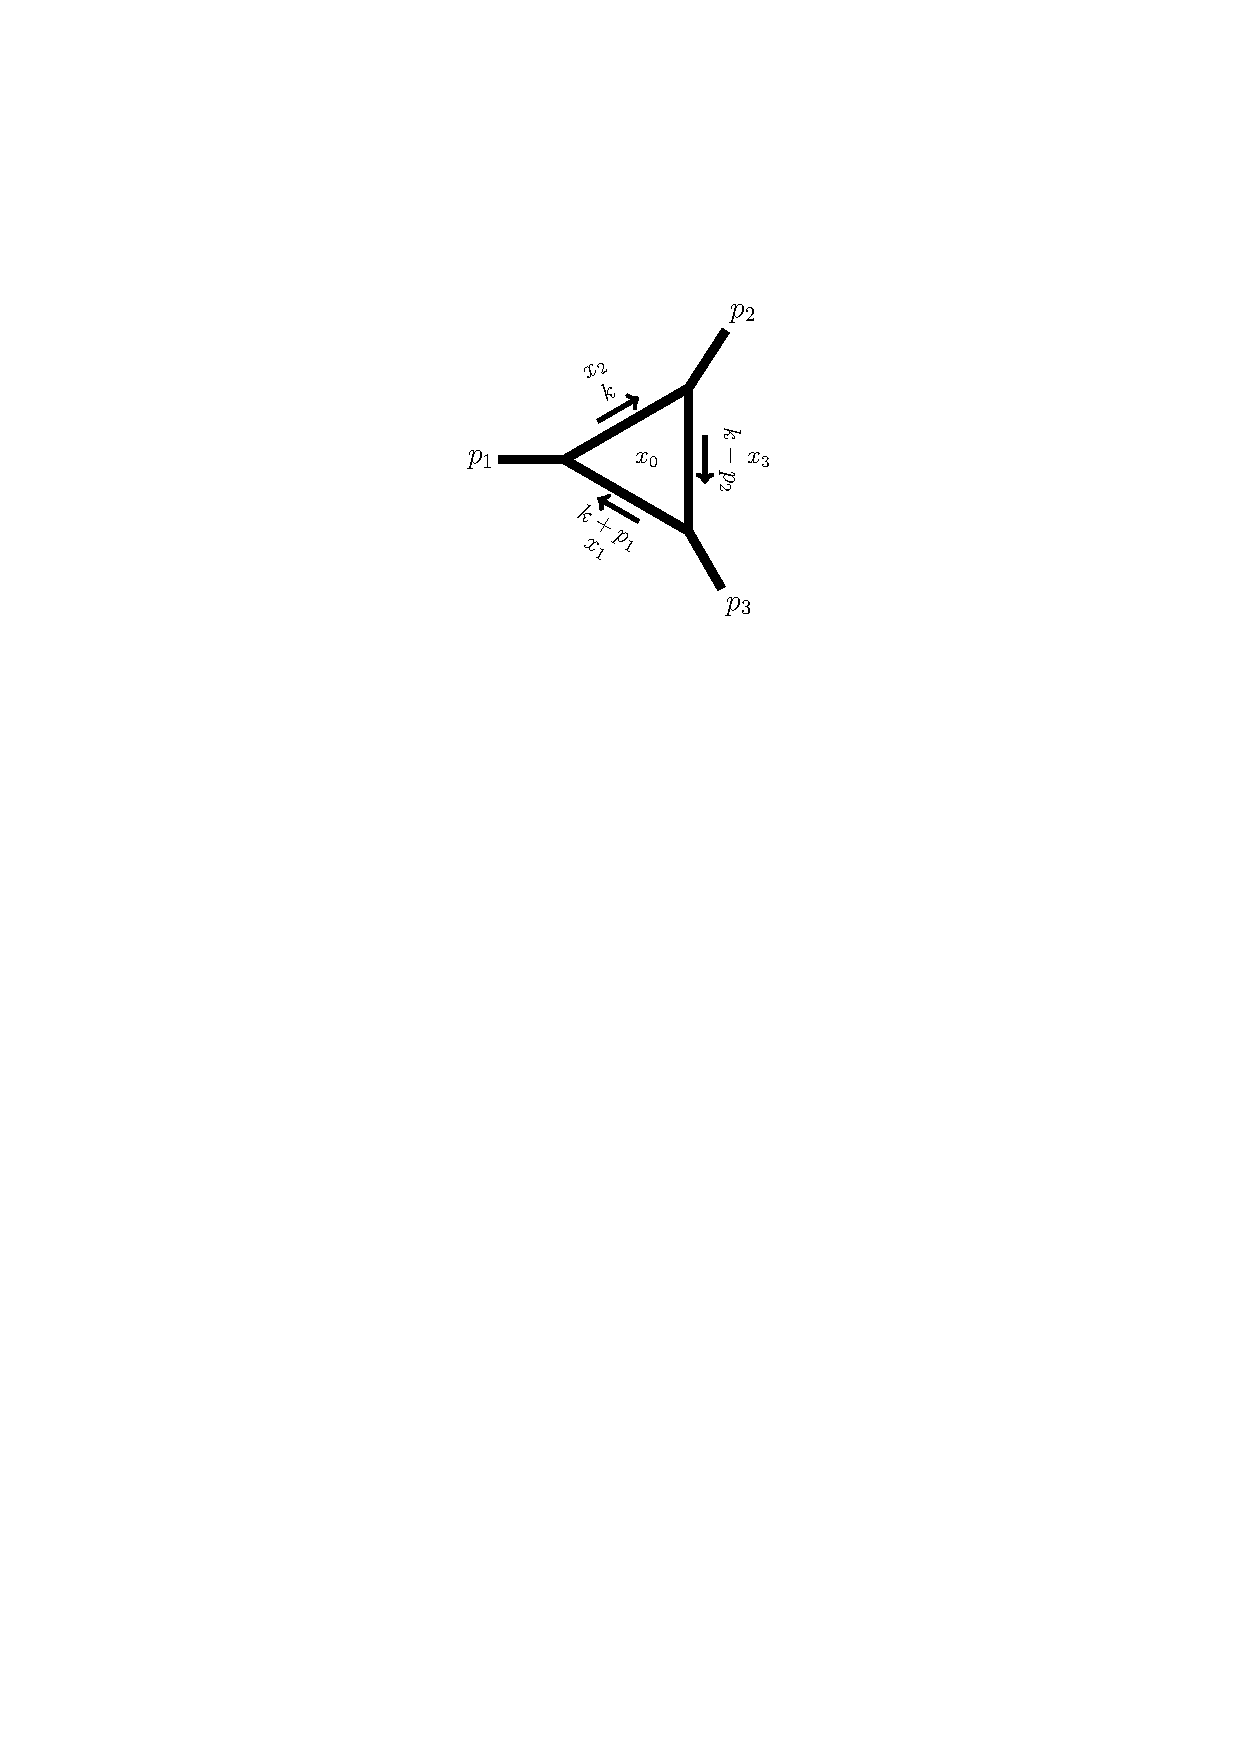
\includegraphics[scale=0.7]{chextra_solutions/figures/triangle_integral.pdf}
\centering
\caption{Diagram of the triangle Feynman integral $F_3$ defined in eq.~(\ref{F3examplemomentumspace}). We write next to each internal edge the corresponding momentum. The arrows denote the directions of the momenta. The edges of the graph divide the space into four regions, which we label by the dual coordinates $x_i$.} 
\label{fig:triangle}
\end{figure}
%
The loop momenta are then given by
\begin{align} \label{eq:props2x}
k = x_0 - x_2 \,, \quad \quad k+p_1 = x_0 - x_1 \,, \quad \quad k-p_2 = x_0 - x_3 \,,
\end{align}
so that the integral takes the form of \eqn{oneloop_dual},
\begin{align} \label{eq:F3dual}
F_3 = \int \frac{\d^D x_0}{\i \pi^{D/2}} \prod_{j=1}^3 \frac{1}{- x^2_{0j} - \i 0} \,.
\end{align}
The relation between the loop momentum $k$ and the dual variables in \eqn{eq:props2x} differs from that given in \eqn{eq:dual_coordinates}, $k=x_1-x_0$. We emphasise that this is just a convention, as we are free to redefine the loop integration variables. The dual regions, on the other hand, are invariant. 
This means that once we assign coordinates $x_i$ to the dual regions, the integral takes the 
form of \eqn{eq:F3dual} (in agreement with the general formula~\eqref{oneloop_dual}),
regardless of the loop-momentum labelling we started from.

The kinematic constraints $p_1^2 = p_2^2 = 0$ and $p_3^2 = s$ imply that
\begin{align}
x^2_{12} = p_1^2 = 0 \,, \qquad x^2_{23} = p_2^2 = 0 \,, \qquad x^2_{13} = p_3^2 = s \,,
\end{align}
as claimed. 
%
The Symanzik polynomials are given by
\begin{align}
U = \alpha_1 + \alpha_2 + \alpha_3 \,, \qquad V = - s \, \alpha_1 \alpha_3 \,.
\end{align}
Substituting the above into \eqn{eq:F3dual} with $D=4-2 \eps$ 
gives the following Feynman parameterisation:
\begin{align}
F_3 = \Gamma(1+\eps) \int_0^{\infty} \frac{\d \alpha_1 \d \alpha_2 \d \alpha_3}{\text{GL}(1)} 
  \frac{1}{(\alpha_1+\alpha_2+\alpha_3)^{1-2\eps} (- s \, \alpha_1 \alpha_3 - \i 0)^{1+\eps} } \,.
\end{align}

%================================================

\section*{Exercise \ref{Ex:TaylorLogGamma}: Taylor series of the Log-Gamma function}
\label{Sol:TaylorLogGamma}
\begin{enumerate}[a)]
\item The recurrence relation of the digamma function follows from that of the $\Gamma$ function~\eqref{eq:gammarecurrence}. 
Differentiating the latter, and dividing both sides by $x \Gamma(x)$ gives
\begin{align}
\frac{ \Gamma'(x+1)}{\Gamma(x+1)} = \frac{1}{x} + \frac{\Gamma'(x)}{\Gamma(x)} \,,
\end{align}
where we have used $x \Gamma(x) = \Gamma(x+1)$.
Comparing to the definition of the digamma function in \eqn{eq:psidef}, we can rewrite this as
\begin{align} \label{eq:psirecurrence}
\psi(x+1) = \frac{1}{x} + \psi(x) \,.
\end{align}
We apply \eqn{eq:psirecurrence} recursively starting from $\psi(x+n)$ with $n\in\mathbb{N}$,
\begin{align}
\begin{aligned}
\psi(x+n) & = \frac{1}{x+n-1} + \psi(x+n-1) \\
& = \frac{1}{x+n-1} + \frac{1}{x+n-2} + \psi(x+n-2)  \\
& = \sum_{s=1}^n \frac{1}{x+n-s} + \psi(x) \,.
\end{aligned} 
\end{align}
Changing the summation index to $k=n-s$ in the last line gives \eqn{eq:psixn}.

\smallskip 

\item Consider the difference $\psi(x+n) - \psi(1+n)$. Using \eqn{eq:psixn} we can rewrite it as
\begin{align} \label{eq:psidiff}
\psi(x+n) - \psi(1+n) = \sum_{k=0}^{n-1} \left(\frac{1}{x+k} - \frac{1}{1+k}\right) + \psi(x) + \gamma_{\text{E}} \,,
\end{align}
where we recall that $\psi(1) = - \gamma_{\text{E}}$. In order to study the limit $n \to \infty$ we use Stirling's formula~\eqref{eq:stirling}, which implies the following approximation for $\psi(x)$,
\begin{align}
\psi(1+x) = \frac{1}{2 x} + \log(x) + \mathcal{O}\left(\frac{1}{x^2}\right) \,.
\end{align}
It follows that 
\begin{align}
\lim_{n\to \infty} \left[ \psi(x+n) - \psi(1+n) \right] = 0 \,.
\end{align}
Taking the limit $n\to \infty$ of both sides of \eqn{eq:psidiff} gives \eqn{eq:psiseries}.

\smallskip

\item 
The series series representation~\eqref{eq:psiseries} of the digamma function allows us the compute the higher-order derivatives in the Taylor expansion~\eqref{eq:loggammataylorgen},
\begin{align} \label{eq:dndloggamma}
\begin{aligned}
\frac{\d^n}{\d x^n} \log \Gamma(1+x) \biggl|_{x=0}  & = \frac{\d^{n-1}}{\d x^{n-1}} \psi(1+x) \biggl|_{x=0} \\
& = (-1)^n \, (n-1)! \, \sum_{k=0}^{\infty} \frac{1}{(1+k)^{n}} \,,
\end{aligned}
\end{align}
for $n\ge 2$.
By changing the summation index to $k'=k+1$, we recognise in the last line the definition of the Riemann zeta constant $\zeta_n$ given in \eqn{eq:zetan}. Substituting \eqn{eq:dndloggamma} into \eqn{eq:loggammataylorgen} and simplifying finally give \eqn{eq:logGammaTaylor}.

\end{enumerate}


%================================================

\section*{Exercise \ref{Ex:4.2Dbubble}: Finite two-dimensional bubble integral}
\label{Sol:4.2Dbubble}
%
We start from the Feynman parameterisation in \eqn{eq:bubbleFeynman}. We set $D=2$, fix the $\text{GL}(1)$ freedom such that $\alpha_1+\alpha_2=1$, and absorb the $\i 0$ prescription in a small positive imaginary part of $s$. We obtain
\begin{align}
F_2\bigl(s,m^2; D=2\bigr) = \int_0^1 \frac{\d \alpha_1}{-s \, \alpha_1 (1-\alpha_1 ) + m^2} \,.
\end{align}
In order to carry out the integration, we factor the denominator and decompose the integrand into partial fractions w.r.t.~$\alpha_1$:
\begin{align}
F_2\bigl(s,m^2; D=2\bigr) = \frac{1}{s \, (\alpha_1^+-\alpha_1^-)} \int_0^1 \d \alpha_1 \left( \frac{1}{\alpha_1 - \alpha_1^+} - \frac{1}{\alpha_1 - \alpha_1^-} \right) \,,
\end{align}
where
\begin{align}
\alpha_1^{\pm} = \frac{1}{2} \left( 1 \pm \sqrt{\Delta} \right) \,, \qquad \Delta = 1 - 4 \, \frac{m^2}{s} \,. 
\end{align}
For $s<0$ and $m^2>0$, we have that $\alpha_1^+ >1$ and $\alpha_1^-<0$. The integration then yields
\begin{align} \label{eq:Bintermediate}
F_2\bigl(s,m^2;D=2\bigr) = \frac{1}{s \, \sqrt{\Delta}} \log \left[ \frac{\alpha_1^- (\alpha_1^+-1)}{\alpha_1^+ (\alpha_1^--1)} \right] \,.
\end{align}
We may simplify the expression by changing variables to $s$ and $x$ through 
\begin{align} \label{eq:m2x}
m^2 = -s \frac{x}{(1-x)^2} \,,
\end{align}
with $0<x<1$. The discriminant $\Delta$ in fact becomes a perfect square, and $\sqrt{\Delta}$ a rational function. The choice of the branch of the square root is arbitrary. We choose
\begin{align} \label{eq:branch_choice}
\sqrt{\Delta} = \frac{1+x}{1-x} \,,
\end{align}
which is positive for $0<x<1$. Equation~\eqref{eq:Bintermediate} then simplifies to
\begin{align} \label{eq:Bintermediate2}
F_2\bigl(s,m^2;D=2\bigr) = \frac{2}{s} \frac{1-x}{1+x} \log(x) \,.
\end{align}

Equation~\eqref{eq:Bintermediate2} is very simple, but hides a symmetry property. We said above that the choice of the branch of $\sqrt{\Delta}$ is arbitrary. In other words, $F_2$ must be invariant under $\sqrt{\Delta} \to - \sqrt{\Delta}$. Let us work out how $x$ changes under this transformation. Solving \eqn{eq:m2x} for $x$ gives two solutions. We choose the one such that $0<x<1$ for $s<0$ and $m^2>0$, which is compatible with \eqn{eq:branch_choice}:
\begin{align}
x = 1 - \frac{1}{2} \frac{s}{m^2} \left(1-\sqrt{\Delta}\right) \,.
\end{align}
One may then verify that $1/x = x \bigl|_{\sqrt{\Delta} \to - \sqrt{\Delta}} $.
Therefore, when changing the sign of $\sqrt{\Delta}$, both the logarithm in \eqn{eq:Bintermediate2} and its coefficient gain a factor of $-1$, so that $F_2$ is indeed invariant. This property is very common in Feynman integrals involving square roots. A particularly convenient way to make it manifest is to rewrite the argument of the logarithm in the form 
\begin{align}
\log\left( \frac{\sqrt{\Delta}-a}{\sqrt{\Delta}+a} \right) \,,
\end{align}
for some rational function $a$. In the triangle case, dimensional analysis tells us that $a$ must be a constant. Indeed, one may verify with $a=1$ we recover $\log(x)$. 
Our final expression for the two-dimensional bubble integral therefore is
\begin{align}
F_2\bigl(s,m^2; D=2\bigr) =  \frac{2}{s \, \sqrt{\Delta}} \log \left(  \frac{\sqrt{\Delta}-1}{\sqrt{\Delta}+1} \right) \,.
\end{align}


%================================================

\section*{Exercise \ref{Ex:ExpGamma}: Laurent expansion of the Gamma function}
\label{Sol:ExpGamma}
\begin{enumerate}[a)]

\item Since $\Gamma(z)$ has a simple pole at $z=0$, $\Gamma(z+1) = z \Gamma(z)$ admits a Taylor expansion around $z=0$,
\begin{align} \label{eq:Gammazp1exp}
\Gamma(z+1) = 1 - z \, \euler + \frac{z^2}{2} \Gamma''(1) + \mathcal{O}\bigl(z^3\bigr) \,.
\end{align}
In order to evaluate the second derivative of $\Gamma(z)$, we relate it to the digamma function through \eqn{eq:psidef}. Then we have that
\begin{align} \label{eq:gammapp1}
\Gamma''(1) = \psi'(1) + \euler^2 \,.
\end{align}
Finally, we can evaluate $\psi'(1)$ using the series representation of the digamma function~\eqref{eq:psiseries}, obtaining
\begin{align} \label{eq:psip1}
\psi'(1) = \sum_{k=0}^{\infty} \frac{1}{(k+1)^2} = \zeta_2 \,.
\end{align}
Substituting eqs.~\eqref{eq:psip1} and~\eqref{eq:gammapp1} into \eqn{eq:Gammazp1exp}, and dividing by $z$ both sides of the equation gives the desired Laurent expansion~\eqref{eq:GammaExp0}.

\smallskip

\item In order to exploit the Laurent expansion around $z=0$ computed in the previous part, we apply the recurrence relation~\eqref{eq:gammarecurrence} iteratively until we get
\begin{align} \label{eq:gammaznrec}
\Gamma(z) =  \frac{\Gamma(z+n)}{z(z+1) \ldots (z+n-1) }  \,.
\end{align}
The Laurent expansion of $\Gamma(z+n)$ around $z=-n$ is then obtained from \eqn{eq:GammaExp0} by replacing $z$ with $z+n$.
The remaining factors are regular at $z=-n$, and their Taylor expansion is given in terms of harmonic numbers~\eqref{eq:harmonicnumbers} by
\begin{align} \label{eq:factorsexp}
\prod_{k=0}^{n-1} \frac{1}{z+k}  =  \frac{(-1)^n}{n!} \left[ 1 + (z+n) \, H_n + \frac{(z+n)^2}{2} \left( H_{n,2} + H_n^2 \right) + \mathcal{O}\left((z+n)^3\right) \right] \,.
\end{align}
Substituting \eqn{eq:GammaExp0} with $z \to z+n$ and \eqn{eq:factorsexp} into \eqn{eq:gammaznrec}, and expanding up to order $(z+n)$ gives \eqn{eq:GammaExpn}.

\end{enumerate}

%================================================

\section*{Exercise \ref{Ex:4.BoxMellinBarnes}: Massless one-loop box with Mellin-Barnes parametrisation}
\label{Sol:4.BoxMellinBarnes}
%
We begin by rewriting the function $B$ in \eqn{eq:MBboxB} as
\begin{align} \label{eq:B2B1}
B = - \frac{2 \, \eps}{t^2} \, B^{(1)} + \mathcal{O}\bigl(\eps^2\bigr) \,,
\end{align}
where
\begin{align} \label{eq:B1def}
B^{(1)} = \int_{\Re(z)=c'} \frac{\d z}{2\pi \i} \, x^{-z} \, \Gamma(-z)^3 \, \frac{\Gamma(1+z)^3}{1+z} \,.
\end{align}
We applied the recurrence relation~\eqref{eq:gammarecurrence} twice---with $n=-1-z$ and $n=1+z$---to simplify the expression w.r.t.~\eqn{eq:MBboxB}. The pole structure of $B^{(1)}$ is depicted in figure~\ref{fig:box_MB_ex}. From the latter we see that $-1 < c' <0$. E.g., we may set $c'=-1/2$.
%
\begin{figure}[t]
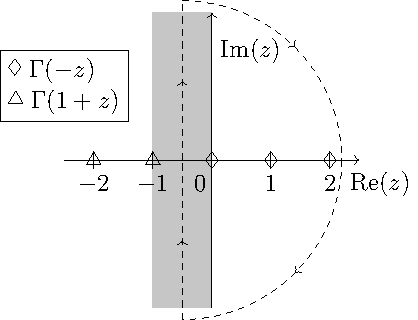
\includegraphics[scale=0.7]{chextra_solutions/figures/box_mellin_barnes_ex.pdf}
\centering
\caption{Pole structure of the $\Gamma$ functions in eq.~(\ref{eq:MBboxB1}), and integration contour (dashed line).}
\label{fig:box_MB_ex}
\end{figure}
%
In order to carry out the integration we close the contour at infinity. Assuming that $x>1$, we close the contour to the right, as shown in figure~\ref{fig:box_MB_ex}. The contribution from the semi-circle at infinity vanishes, and the integral is given by
\begin{align} \label{eq:MBboxB1}
B^{(1)} = - \sum_{n=0}^{\infty}  \text{Res}\left[ x^{-z} \, \Gamma(-z)^3 \, \frac{\Gamma(1+z)^3}{1+z} , \, z=n \right] \,.
\end{align}
The minus sign comes from the clockwise direction of the loop. To compute the residues, we make use of the Laurent expansions computed in exercise~\ref{Ex:ExpGamma}. The factor of $\Gamma(-z)^3$ entails a triple pole at $z=n$ (with $n=0,1,\ldots$), so that we need the expansion of all functions involved around $z=n$ up to the third order. We obtain the Laurent expansion of $\Gamma(-z)$ around $z=n$ by replacing $z\to -z$ in \eqn{eq:GammaExpn},
\begin{align} \label{eq:ExpGammamz}
\Gamma(-z) = \frac{(-1)^n}{n!} \left\{ \frac{-1}{z-n} + H_n-\euler - \frac{z-n}{2} \left[\left(H_n - \euler\right)^2 + \zeta_2 + H_{n,2} \right] \right\} + \ldots \,.\end{align}
In order to compute the Taylor expansion of $\Gamma(1+z)$ we leverage what we learnt about the digamma function in exercise~\ref{Ex:TaylorLogGamma}.
The first derivative is given by
\begin{align}
\frac{\d}{\d z} \Gamma(1+z) \biggl|_{z=n} = \Gamma(1+n) \, \psi(1+n) = n! \, (H_n - \gamma_{\text{E}}) \,,
\end{align}
where we used the recurrence relation~\eqref{eq:psixn}. We recall the definition of the harmonic numbers in \eqn{eq:harmonicnumbers}. For the second derivative we use again \eqn{eq:psixn} to write $\psi'(1+n) = \psi'(1) - H_{n,2}$, and \eqn{eq:psiseries} to evaluate $\psi'(1) = \zeta_2$. We thus obtain
\begin{align}
\frac{\d^2}{\d z^2} \Gamma(1+z) \biggl|_{z=n} =& n! \, \bigl[ \psi(1+n)^2 + \psi'(1+n) \bigl] \nonumber \\
=& n! \, \bigl[ (H_n-\gamma_{\text{E}})^2 + \zeta_2 - H_{n,2} \bigr] \,.
\end{align}
Putting the above together gives the Taylor expansion of $\Gamma(1+z)$ around $z=n$:
\begin{align} \label{eq:ExpGamma1pz}
\Gamma(1+z) = n! \left\{ 1 + (z-n) \bigl( H_n - \gamma_{\text{E}}\bigr) + \frac{(z-n)^2}{2} \bigl[ (H_n-\gamma_{\text{E}})^2+\zeta_2-H_{n,2} \bigr] 
  + \ldots \right\}\,.
\end{align}
Attentive readers may notice that the expansion of $\Gamma(1+z) \Gamma(-z)$ is much simpler:
\begin{align}
\Gamma(-z) \, \Gamma(1+z) = - (-1)^n \, \biggl[ \frac{1}{z-n} + \zeta_2 \, (z-n) \biggr] + \mathcal{O}\bigl((z-n)^2\bigr) \,.
\end{align}
We could have arrived directly at this result through Euler's reflection formula,
\begin{align}
\Gamma(-z) \, \Gamma(1+z) = -\frac{\pi}{\sin(\pi z)} \,.
\end{align}
The Taylor expansions of the other functions in \eqn{eq:B1def} are straightforward.
Substituting them into \eqn{eq:MBboxB1} and taking the residue gives
\begin{align} \label{eq:MBboxB1b}
B^{(1)}  = \sum_{n=0}^{\infty} \frac{(-x)^{-n}}{(1+n)^3} + \log(x) \sum_{n=0}^{\infty} \frac{(-x)^{-n}}{(1+n)^2}  +
  \frac{1}{2} \bigl(\pi^2+\log^2(x)\bigr) \sum_{n=0}^{\infty} \frac{(-x)^{-n}}{1+n} \,.
\end{align}
The series can be summed in terms of polylogarithms through their definition~\eqref{def_polylogarithm_series}:
\begin{align}
\sum_{n=0}^{\infty}  \frac{(-x)^{-n}}{(1+n)^k} = - x \, \mathrm{Li}_k\left(-\frac{1}{x}\right) \,,
\end{align}
for $k=1,2,\ldots$ and $x>1$. Plugging this into \eqn{eq:MBboxB1b}, and the latter into \eqn{eq:B2B1} gives our final expression for $B$:
\begin{align} \label{eq:MBboxBfinal}
B = \frac{2 \, \eps}{s\, t} \, \biggl[ \mathrm{Li}_3\left(-\frac{1}{x}\right) + \log(x) \, \mathrm{Li}_2\left(-\frac{1}{x}\right) -
  \frac{1}{2}\bigl(\pi^2 + \log^2(x)\bigr) \log\left(1+\frac{1}{x}\right) \biggr] + \mathcal{O}\bigl(\eps^2\bigr) \,.
\end{align}
The expression of the massless one-loop box $F_4$ in \eqn{eq:F4final} is obtained by subtracting from $B$ in \eqn{eq:MBboxBfinal} the Laurent expansion of the residue $A$ in \eqn{eq:MBboxA}.


%================================================


\section*{Exercise \ref{Ex:Discontinuities}: Discontinuities}
\label{Sol:Discontinuities}
\begin{enumerate}[a)]

\item The logarithm of a complex variable $z = |z| \text{e}^{\i \, \text{arg}(z)}$ is defined as
\begin{align}
\log(z) = \log|z| + \i \, \text{arg}(z) \,,
\end{align}
where $|z|$ is the absolute value of $z$, and the argument of $z$ ($\text{arg}(z)$) is the counterclockwise angle from the positive real axis to the line connecting $z$ with the origin. $\log|z|$ is a continuous function of $z$, hence the discontinuity of $\log(z)$ originates from $\text{arg}(z)$. As $z$ approaches the negative real axis from above (below), $\text{arg}(z)$ approaches $\pi$ ($-\pi$). In other words, we have that
\begin{align}
 \lim_{\eta\to 0^+}\text{arg} (x \pm \i \eta) = \pm \pi \, \Theta(-x)  \,,
\end{align}
for $x \in \mathbb{R}$.
The discontinuity of the logarithm across the real axis is thus given by
\begin{align}
\begin{aligned}
\text{Disc}_x \left[ \log (x) \right] & = \lim_{\eta\to 0^+} \i \left[ \text{arg}(x+\i \eta) -  \text{arg}(x-\i \eta) \right] \\
 & = 2\i \pi \, \Theta(-x) \,.
 \end{aligned}
\end{align}

\item We rewrite the identity~\eqref{eq:Li2identity} here for convenience:
\begin{align} \label{eq:Li2identitySol}
{\rm Li}_2(x) = - {\rm Li}_2(1-x) - \log(1-x) \log(x) + \zeta_2 \,.
\end{align}
This equation is well defined for $0<x<1$. 
Focusing on the RHS, however, we see that all functions are well defined for $x>0$ except for $\log(1-x)$.
We can thus make use of \eqn{eq:Li2identitySol} to reduce the analytic continuation of ${\rm Li}_2(x)$ to $x>1$ 
to that of $\log(1-x)$. For $x>1$ we have that
\begin{align}
{\rm Li}_2(x + \i \eta) - {\rm Li}_2(x - \i \eta) = \log(x) \left[ \log(1-x+\i \eta ) - \log(1-x-\i \eta) \right] + \mathcal{O}(\eta) \,.
\end{align}
Hence, the discontinuity of the dilogarithm follows from that of the logarithm, as
\begin{align}
\text{Disc}_x \left[ {\rm Li}_2 (x) \right] & = \log (x) \, \text{Disc}_x \left[ \log(1-x) \right]  \nonumber \\
& = 2 \pi \i \, \log(x) \, \Theta(x-1) \,.
\end{align}

\end{enumerate}



%================================================


\section*{Exercise \ref{Ex:4.Symbol}: The symbol of a transcendental function}
\label{Sol:4.Symbol}
%
We make use of the recursive definition of the symbol~\eqref{defsymbol2}. 
The differential of $\log(x) \log (1-x)$ is given by
\begin{align}
\d \left[ \log(x) \log (1-x) \right] =  \log (1-x) \, \d \log(x) +  \log (x) \, \d \log (1-x)  \,.
\end{align}
Through \eqn{defsymbol2} we then have that 
\begin{align}
\mathcal{S}\bigl( \log(x) \log (1-x) \bigr) = [ S(\log(1-x)) , x ] + [ S(\log(x)), 1-x] \,.
\end{align}
Since we already know that $S(\log a) = [a]$ (\eqn{eq:symbol_log}), the final result is
\begin{align} \label{eq:sloglog1}
\mathcal{S}\bigl( \log(x) \log (1-x) \bigr) = [x, 1-x] + [1-x, x] \,.
\end{align} 
%
Alternatively, one may replace each function in the product by its symbol,
\begin{align} \label{eq:sloglog2}
\mathcal{S}\bigl( \log(x) \log (1-x) \bigr) = [x] \times [1-x]  \,.
\end{align}
By comparing \eqn{eq:sloglog1} and \eqn{eq:sloglog2} we see that
\begin{align}
[x] \times [1-x] = [x,1-x] + [1-x, x] \,.
\end{align}
This is a very important property of the symbol called \emph{shuffle product}. It allows us to express the product of two symbols of weights $n_1$ and $n_2$ as a linear combination of symbols of weight $n_1+n_2$. For example, at weight three we have
\begin{align}
[a] \times [b,c] = [a,b,c] + [b,a,c] + [b,c,a] \,.
\end{align}
We refer the interested readers to ref.~\cite{ch5-Duhr:2019tlz}.


%================================================

\section*{Exercise \ref{Ex:4.W2basis}: Symbol basis and weight-two identities}
\label{Sol:4.W2basis}
\noindent
a) The symbol method turns finding relations among special functions into a linear algebra problem. The first step is to put the symbols of \eqn{eq:symbolbasisweight2} and the functions of \eqn{eq:funcbasisW2} in two vectors:
\begin{align}
& \vec{b} = \bigl( [x,x] , [x,1-x], [1-x,x], [1-x,1-x] \bigr)^{\top} \,, \\
& \vec{g} = \bigl( \log^2(x),  \log^2 (1-x),  \log(x) \log (1-x),  {\rm Li}_{2}(1-x) \bigr)^{\top} \,.
\end{align}
The elements of $\vec{b}$ are a basis of all weight-two symbols in the alphabet $\{x, 1-x\}$. We can thus express the symbol of $\vec{g}$ in the basis $\vec{b}$, as
\begin{align}
\mathcal{S}(\vec{g}) = \begin{pmatrix} 
2 \, [x,x] \\
2 \, [1-x,1-x] \\
[x,1-x]+[1-x,x] \\
- [x,1-x] \\
\end{pmatrix} = M \cdot \vec{b} \,, \qquad \text{with} \quad 
M = \begin{pmatrix}
2 & 0 & 0 & 0 \\
0 & 0 & 0 & 2 \\
0 & 1 & 1 & 0 \\
0 & -1 & 0 & 0 \\
\end{pmatrix} \,.
\end{align}
Since the matrix $M$ has non-zero determinant, we can invert it to express the weight-two symbol basis $\vec{b}$ in terms of the symbols of the functions in $\vec{g}$,
\begin{align} \label{eq:b2g}
\vec{b} = M^{-1} \cdot \mathcal{S}(\vec{g}) \,, \qquad \text{with} \quad 
M^{-1} = \begin{pmatrix}
\frac{1}{2} & 0 & 0 & 0 \\
0 & 0 & 0 & -1 \\
0 & 0 & 1 & 1 \\
0 & \frac{1}{2} & 0 & 0 \\
\end{pmatrix} \,.
\end{align}
Therefore, $\vec{g}$ is a basis of the weight-two symbols in the alphabet $\{x,1-x\}$ as well.

\smallskip
\noindent
b) Let us start from ${\rm Li}_{2}\left(x/(x-1)\right)$. Using \eqn{eq:Li2symbolexample}, its symbol is given by
\begin{align}
\mathcal{S}\biggl[{\rm Li}_{2}\left(\frac{x}{x-1}\right)\biggr] = - \left[1-\frac{x}{x-1}, \frac{x}{x-1} \right] \,.
\end{align}
The properties~\eqref{eq:symbol_properties} allow us to express the latter in terms of the letters $\{x,1-x\}$:
\begin{align}
\mathcal{S}\biggl[{\rm Li}_{2}\left(\frac{x}{x-1}\right)\biggr] = [1-x, x ] - [1-x, 1-x] \,.
\end{align}
We can then express the symbol of ${\rm Li}_{2}(x/(x-1))$ in the basis $\vec{b}$, as
\begin{align}
\mathcal{S}\biggl[{\rm Li}_{2}\left(\frac{x}{x-1}\right)\biggr] = (0, 0, 1, -1) \cdot \vec{b} \,.
\end{align}
In this sense, ${\rm Li}_{2}(x/(x-1))$ `lives' in the space spanned by \eqn{eq:symbolbasisweight2}. 
We do the same for the other dilogarithms in \eqn{eq:dilogs}:
\begin{align}
& \mathcal{S}\bigl[ {\rm Li}_{2}(x) \bigr] = - [1-x,x] = (0, 0, -1, 0) \cdot \vec{b} \,, \\ 
& \mathcal{S}\biggl[ {\rm Li}_{2}\left(\frac{1}{x}\right)\biggr]  = [1 - x, x] - [x, x] = (-1, 0, 1, 0) \cdot \vec{b} \,, \\
& \mathcal{S}\biggl[  {\rm Li}_{2}\left(\frac{1}{1-x}\right)\biggr]  = -[1 - x, 1 - x] + [x, 1 - x] = (0, 1, 0, -1) \cdot \vec{b} \,, \\ 
& \mathcal{S}\biggl[  {\rm Li}_{2}\left(\frac{x-1}{x} \right)\biggr]  = [x, 1 - x] - [x, x] = (-1, 1, 0, 0) \cdot \vec{b} \,. 
\end{align}

\smallskip
\noindent
c) Having expanded the symbols of the dilogarithms in \eqn{eq:dilogs} in the basis $\vec{b}$, 
we can change basis from $\vec{b}$ to $\mathcal{S}(\vec{g})$ as in \eqn{eq:b2g}. For example, we have
\begin{align} \begin{aligned}
\mathcal{S}\biggl[{\rm Li}_{2}\left(\frac{x}{x-1}\right)\biggr] & = (0, 0, 1, -1) \cdot M^{-1} \cdot S(\vec{g}) \\
& = \mathcal{S}\biggl[-\frac{1}{2} \log^2 (1-x) + \log(x) \log (1-x) + {\rm Li}_{2}(1-x) \biggl] \,.
\end{aligned} \end{align}
Doing the same for the other dilogarithms in \eqn{eq:dilogs} gives the following identities:
\begin{align}
& \mathcal{S}\biggl[  {\rm Li}_{2}(x) + {\rm Li}_{2}(1 - x) + \log(x) \log(1 - x)  \biggr] = 0 \,, \\
& \mathcal{S}\biggl[ {\rm Li}_{2}\left(\frac{1}{x}\right) - {\rm Li}_{2}(1 - x)  - \log(x) \log(1 - x) + \frac{1}{2} \log^2(x) \biggr] = 0 \,, \\
& \mathcal{S}\biggl[ {\rm Li}_{2}\left(\frac{1}{1-x}\right) + {\rm Li}_2(1 - x)  + \frac{1}{2} \log^2(1 - x) \biggr] = 0 \,, \\
& \mathcal{S}\biggl[  {\rm Li}_{2}\left(\frac{x-1}{x} \right) + {\rm Li}_2(1 - x) + \frac{1}{2} \log^2(x) \biggr] = 0 \,.
\end{align}
The terms which are missed by the symbol may be fixed as done for \eqn{defgexamplesymbol}.

%================================================

\section*{Exercise \ref{Ex:4.Symbolf2}: Simplifying functions using the symbol}
\label{Sol:4.Symbolf2}
%
We compute the symbol of $f_1(u,v)$ in \eqn{examplef1}. The general strategy is the following:
we use the rule in \eqn{eq:Li2symbolexample} for the dilogarithms; next, we put all letters over a common denominator and factor them; finally, we use the symbol properties~\eqref{eq:symbol_properties} to expand the symbol until all letters are irreducible factors.
This gives
\begin{align}
& \mathcal{S}\biggl[ {\rm Li}_2\left(\frac{1-v}{u}\right) \biggr] = [u+v-1,u] - [u+v-1, 1-v] + [u,1-v] - [u,u] \,, \\
& \begin{aligned}
\mathcal{S}\biggl[ {\rm Li}_2\left(\frac{(1-u)(1-v)}{u v}\right) \biggr] = \ & \bigl( [u+v-1,u]-[u+v-1,1-u]+[u,1-u] \\
&  +[u,1-v]-[u,u]-[u,v] \bigr) + \bigl(u \leftrightarrow v \bigr) \,.
\end{aligned} \end{align}
${\rm Li}_2((1-u)/v)$ is obtained from ${\rm Li}_2((1-v)/u)$ by exchanging $u \leftrightarrow v$, and so is its symbol. The symbol of $\pi^2/6$ vanishes.
Putting the above together gives
\begin{align} \label{eq:Sf1}
\mathcal{S}\bigl[ f_1(u,v) \bigr] = [u, 1 - u] + [v, 1 - v] - [u, v] - [v, u] \,,
\end{align}
as claimed. Note that the letter $u+v-1$ drops out in the sum. In other words, $u+v=1$ is a branch point for the separate terms in the expression of $f_1(u,v)$ given in \eqn{examplef1}, but not for $f_1(u,v)$.

On the RHS of \eqn{eq:Sf1} we recognise in $ [u, 1 - u] $ ($[v, 1 - v]$) the symbol of $-{\rm Li}_2(u)$ ($-{\rm Li}_2(v)$), 
and in $[u, v] + [v, u]$ the symbol of $\log u \log v$ (see exercise~\ref{Ex:4.Symbol}). 
An alternative and simpler expression for $f_1(u,v)$ is thus given by
\begin{align}
\mathcal{S}\bigl[f_1(u,v)\bigr] =\mathcal{S}\bigl[  -{\rm Li}_2(u) -{\rm Li}_2(v) - \log u \log v \bigr] \,,
\end{align}
which matches---at symbol level---the expression of $f_2(u,v)$ in \eqn{examplef1b}.


%================================================

\section*{Exercise \ref{Ex:4.Kite}: The massless two-loop kite integral}
\label{Sol:4.Kite}
We define the integral family as
\begin{align} \label{eq:kitefamily}
G^{\text{kite}}_{a_1,a_2,a_3,a_4,a_5} \coloneqq \int \frac{\d^D k_1}{\i \pi^{D/2}} \frac{\d^D k_2}{\i \pi^{D/2}}
   \frac{1}{D_1^{a_1} D_2^{a_2} D_3^{a_3} D_4^{a_4} D_5^{a_5}} \,,
\end{align}
where the inverse propagators $D_i$ are given by\footnote{In chapter~\ref{ch:loopints} we write the inverse propagators as $D_a = -(k-q_a)^2 + m_a^2 - \i 0 $, which is natural for the loop integration (see section~\ref{sec:ConventionsCh4}), as opposed to $D_a = +(k-q_a)^2 - m_a^2 + \i 0$. We used the latter in chapter~\ref{ch:loopamps} as it is more convenient for the unitarity methods.}
\begin{align} \label{eq:D2sp}
\begin{array}{lll}
D_1 = - k_1^2 \,,  & D_2 = -(k_1-p)^2 \,, \quad \quad & D_3 = -k_2^2 \,, \\
D_4 = -(k_2+p)^2\,, \quad \quad & D_5 = -(k_1+k_2)^2\,. & \\
\end{array}
\end{align}
Feynman's $\i 0$ prescription is dropped, as it plays no part here. The desired integral is
\begin{align}
F_{\text{kite}}\bigl(s; D\bigr) = G^{\text{kite}}_{1,1,1,1,1} \,.
\end{align}
The IBP relations for the triangle sub-integral with loop momentum $k_2$ are given by
\begin{align}
\int \frac{\d^D k_1}{\i \pi^{D/2}} \frac{\d^D k_2}{\i \pi^{D/2}} \frac{\partial}{\partial k_2^{\mu}}  
   \frac{ q^{\mu} }{D_1 D_2 D_3 D_4 D_5}  = 0 \,,
\end{align}
for any momentum $q$. Upon differentiating we rewrite the scalar products in terms of inverse propagators---and thus of integrals of the family~\eqref{eq:kitefamily}---by inverting the system of equations~\eqref{eq:D2sp} (e.g.\ $k_1 \cdot p =( D_2 - D_1 + s)/2$). 
There are three independent choices for $q$: $k_1$, $k_2$, and $p$. We need to find a linear combination of these such that the resulting IBP relation contains only $F_{\text{kite}}$ and bubble-type integrals. Using $q=k_1+k_2$ gives
\begin{align}
(D-4) \, G^{\text{kite}}_{1, 1, 1, 1, 1} & - G^{\text{kite}}_{1, 1, 1, 2, 0} - 
 G^{\text{kite}}_{1, 1, 2, 1, 0} + G^{\text{kite}}_{0, 1, 2, 1, 1} + G^{\text{kite}}_{1, 0, 1, 2, 1}  = 0 \,.
 \end{align}
The graph symmetries imply that 
\begin{align}
G^{\text{kite}}_{1, 1, 1, 2, 0} = G^{\text{kite}}_{1, 1, 2, 1, 0} \,, \qquad \quad  G^{\text{kite}}_{1, 0, 1, 2, 1} = G^{\text{kite}}_{0, 1, 2, 1, 1} \,.
\end{align}
$G^{\text{kite}}_{1, 1, 2, 1, 0}$ is a product of bubble integrals. Using \eqn{eq:Ibubblechapter4} for the latter gives 
\begin{align}
G^{\text{kite}}_{1, 1, 2, 1, 0} = B(1,1) \, B(1,2) \, (-s)^{D-5} \,.
\end{align}
$G^{\text{kite}}_{0, 1, 2, 1, 1}$ instead has a bubble sub-integral. By using \eqn{eq:Ibubblechapter4} iteratively we obtain
\begin{align}
\begin{aligned}
G^{\text{kite}}_{0, 1, 2, 1, 1} & = \ \vcenter{\hbox{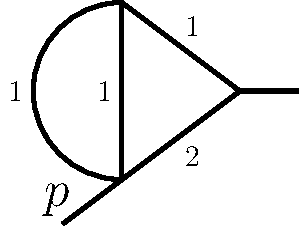
\includegraphics[width=2.5cm]{chextra_solutions/figures/kite_01211.pdf}}}  \\
& = B(1,1) \times \vcenter{\hbox{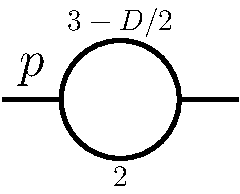
\includegraphics[width=2.cm]{chextra_solutions/figures/kite_bubble.pdf}}}  \\
& = B(1,1) \, B\left(3-\frac{D}{2},2\right) \, (-s)^{D-5} \,,
\end{aligned}
\end{align}
where the numbers next to the propagators in the graphs are their exponents. 
Putting the above together gives
\begin{align}
G^{\text{kite}}_{1, 1, 1, 1, 1} = \frac{2}{D-4} \, B(1,1) \left[ B(1,2) -B\left(3-\frac{D}{2}, 2\right) \right] (-s)^{D-5} \,,
\end{align}
which can be expressed in terms of gamma functions through \eqn{eq:Bbubble}. Setting $D=4-2\eps$ and expanding the $\Gamma$ functions around $\eps=0$ through \eqn{eq:logGammaTaylor} finally gives \eqn{eq:kite_result}.


%================================================

\section*{Exercise \ref{Ex:4.BubbleCut}: ``$\d \log$'' form of the massive bubble integrand with $D=2$}
\label{Sol:4.BubbleCut}
%
We start from the integrand $\omega_{1,1}$ in the first line of \eqn{eq:bubble_dlog}. We use the parameterisation $k = \beta_1 p_1 + \beta_2 p_2$, with $p=p_1+p_2$, $p_1^2=p_2^2=0$ and $2 \, p_1 \cdot p_2 = s$.
We change integration variables from $k$ to $\beta_1$ and $\beta_2$.
The propagators are given~by
\begin{align} \label{eq:prop_beta} \begin{aligned}
& -k^2 + m^2 = -s \, \bigl( \beta_1 \beta_2 - x \bigr) \,, \\
& -(k+p)^2 + m^2 = -s \, \bigl[ (1+\beta_1)(1+\beta_2) - x \bigr] \,,
\end{aligned} \end{align}
where we introduced the short-hand notation $x=m^2/s$.
The Jacobian factor is a function of $s$, and dimensional analysis tells us that $J\propto s$. The constant prefactor is irrelevant here.\footnote{For an example of how to compute the Jacobian factor, see the solution to exercise~\ref{Ex:4.KiteLS}.}
The integrand then reads
\begin{align} \label{eq:ometa11beta}
\omega_{1,1} \propto \frac{1}{s} \, \frac{\d \beta_1 \d \beta_2}{(\beta_1 \beta_2 - x) \bigl[ (1+\beta_1)(1+\beta_2)-x\bigr]} \,.
\end{align}
Our goal is to rewrite $\omega_{1,1}$ in a ``$\d \log$'' form. First, we decompose $\omega_{1,1}$ into partial fractions w.r.t.~$\beta_2$:
\begin{align}
s \, \omega_{1,1} \propto \frac{\d \beta_1}{\beta_1^2 + \beta_1 + x} \, \frac{\d \beta_2}{\beta_2 - x/\beta_1} - 
  \frac{\d \beta_1}{\beta_1^2 + \beta_1 + x} \, \frac{\d \beta_2}{\beta_2 + 1 - x/(1+\beta_1)} \,.
\end{align}
We then push all $\beta_2$-dependent factors into $\d \log$ factors, obtaining
\begin{align} \begin{aligned}
s \, \omega_{1,1} & \propto \frac{\d \beta_1}{\beta_1^2 + \beta_1 + x} \, \d \log\left(\beta_2 - \frac{x}{\beta_1} \right) - 
  \frac{\d \beta_1}{\beta_1^2 + \beta_1 + x} \, \d \log\left(1+\beta_2 - \frac{x}{1+\beta_1} \right)  \\
 & \propto  \frac{\d \beta_1}{\beta_1^2 + \beta_1 + x} \, \d \log \left( \frac{\beta_1 \beta_2 - x}{(1 + \beta_1)(1 + \beta_2) - x} \right) \,.
\end{aligned} \end{align}
In order to do the same w.r.t.~$\beta_1$, we need to factor the polynomial in the denominator:
\begin{align} \label{eq:beta1pm}
\beta_1^2 + \beta_1 + x = \bigl(\beta_1 - \beta_1^+ \bigr) \bigl(\beta_1 - \beta_1^- \bigr) \,, \qquad \beta_1^{\pm} = \frac{1}{2} \Bigl(-1 \pm \sqrt{1-4 x} \Bigr) \,.
\end{align}
Partial fractioning w.r.t.~$\beta_1$ and rewriting all $\beta_1$-dependent factors into $\d \log$'s yields
\begin{align} \label{eq:omega11dlogbeta}
\omega_{1,1} \propto \frac{1}{s \, \sqrt{1-4 x}} \, \d\log\left( \frac{\beta_1 - \beta_1^+}{\beta_1 - \beta_1^-} \right) \, \d \log \left( \frac{\beta_1 \beta_2 - x}{(1 + \beta_1)(1 + \beta_2) - x} \right) \,.
\end{align}
Note that there is a lot of freedom in the expression of the $\d \log$ form. For instance, we might have started with a partial fraction decomposition w.r.t.~$\beta_1$, and we would have obtained a different---yet equivalent---expression. While the expression of the $\d \log$ form may vary, all singularities are always manifestly of the type $\d x/x$, and the leading singularities stay the same (up to the irrelevant sign). 

\smallskip

We now consider the momentum-space $\d \log$ form in \eqn{eq:bubble_dlog}, namely
\begin{align} \label{eq:omega11mom}
\omega_{1,1} \propto \frac{1}{s \, \sqrt{1-4x }} \, \d \log(\tau_1) \, \d \log(\tau_2) \,,
\end{align}
where
\begin{align} \label{eq:taus}
\tau_1 = \frac{-k^2+m^2}{(k-k_{\pm})^2} \,, \qquad \qquad \tau_2 = \frac{-(k+p)^2+m^2}{(k-k_{\pm})^2} \,.
\end{align}
We rewrite the latter in terms of $\beta_1$ and $\beta_2$, and show that it matches \eqn{eq:ometa11beta}.
We recall that $\d = \d\beta_1 \, \partial_{\beta_1} + \d\beta_2 \, \partial_{\beta_2}$ and $\d \beta_2 \, \d \beta_1 = - \d \beta_1 \, \d \beta_2$, which imply that
\begin{align} \label{eq:dk2dbeta}
\d \log(\tau_1) \, \d \log(\tau_2) = \left( \frac{\partial \tau_1}{\partial \beta_1} \frac{\partial \tau_2}{\partial \beta_2} - 
   \frac{\partial \tau_1}{\partial \beta_2} \frac{\partial \tau_2}{\partial \beta_1} \right) \frac{\d \beta_1 \, \d \beta_2}{\tau_1 \, \tau_2} \,.
\end{align}
In \eqn{eq:taus}, $k_{\pm}$ denotes either of the two solutions to the cut equations.
We choose $k_+ = \beta_1^+ \, p_1 + \beta_2^+ \, p_2$, where $\beta_{1}^+$ is given by \eqn{eq:beta1pm} and $\beta_2^+=x/\beta_1^+$. We then have
\begin{align} \label{eq:kmkp}
(k-k_+)^2  = \frac{s}{2} \, \Bigl[2x+\beta_1 + \beta_2 + 2 \beta_1 \beta_2 + (\beta_1 - \beta_2) \sqrt{1 - 4 x} \Bigr]\,.
\end{align}
We substitute eqs.~\eqref{eq:kmkp} and~\eqref{eq:prop_beta} into \eqn{eq:taus}, and the latter into \eqn{eq:dk2dbeta}. Simplifying the result---possibly with a computer-algebra system---gives 
\begin{align}
\frac{1}{s \, \sqrt{1-4x }} \, \d \log(\tau_1) \, \d \log(\tau_2) = \frac{1}{s} \, \frac{\d\beta_1 \, \d \beta_2}{(\beta_1 \beta_2 - x) \bigl[(1 + \beta_1)(1 + \beta_2) - x \bigr] } \,,
\end{align}
which matches the expression of $\omega_{1,1}$ in \eqn{eq:ometa11beta}, as claimed.

%================================================

\section*{Exercise \ref{Ex:4.KiteLS}: An integrand with double poles: the two-loop kite in $D=4$}
\label{Sol:4.KiteLS}
%
We complement $p_1$ and $p_2$ with two momenta constructed from their spinors,
\begin{align}
p_3^{\mu} = \frac{1}{2} \spAB{1}{\gamma^{\mu}}{2} \,, \quad p_4^{\mu} = \frac{1}{2} \spAB{2}{\gamma^{\mu}}{1} \,,
\end{align}
to construct a four-dimensional basis. We have that $p_1 \cdot p_2  = - p_3 \cdot p_4 = s/2$,
while all other scalar products $p_i \cdot p_j$ vanish. We expand the loop momenta as
\begin{align}
k_1^{\mu} = \sum_{i=1}^4 a_i \, p_i^{\mu} \,, \qquad k_2^{\mu} = \sum_{i=1}^4 b_i \, p_i^{\mu} \,,
\end{align}
and change integration variables from $k_1^{\mu}$ and $k_2^{\mu}$ to $a_i$ and $b_i$. 
The inverse propagators defined in \eqn{eq:D2sp} are given by
\begin{align}\label{eq:D2ab}
\begin{aligned}
& \begin{array}{ll}
D_1 = \left(a_3 a_4 - a_1 a_2\right) s \,, \qquad \qquad & D_2 = \left(a_3 a_4 - a_1 a_2 + a_1 + a_2  -1 \right) s \,, \\
D_3 = \left(b_3 b_4 - b_1 b_2\right) s \,, \qquad \qquad & D_4 = \left(b_3 b_4 - b_1 b_2 - b_1 - b_2  -1 \right) s \,, \\
\end{array} \\
& \, D_5 = \left(a_3 a_4 - a_1 a_2 + b_3 b_4  - b_1 b_2 + a_3 b_4 + a_4 b_3 - a_1 b_2 - a_2 b_1 \right) s   \,.
\end{aligned}
\end{align}
The Jacobian $|J_1|$ of the change of variables $\{k_1^{\mu}\} \to \{a_i\}$ is the determinant of the $4 \times 4$ matrix with entries
\begin{align}
\left(J_1\right)^{\mu}_i = \frac{\partial k_1^{\mu}}{\partial a_i} \,, \quad \mu=0,\ldots,3 \,, \quad i=1,\ldots, 4\,.
\end{align}
Dimensional analysis tells us that $|J_1| \propto s^2$. It is instructive to compute it explicitly as well.
To do so, it is convenient to first consider
\begin{align}
\left(J_1\right)^{\mu}_i \eta_{\mu \nu} \left(J_1\right)^{\nu}_j = p_i \cdot p_j \,.
\end{align}
Taking the determinant on both sides gives
\begin{align}
|J_1|^2 = - \frac{s^4}{16}\,,
\end{align}
where the minus sign comes from the determinant of the metric tensor. The Jacobian for  $\{k_2^{\mu}\} \to \{b_i\}$ is similar.
The maximal cut is then given by
\begin{align}
F_{\text{kite}}^{\text{max cut}} \propto s^4 \int \d a_1 \d a_2 \d a_3 \d a_4 \d b_1 \d b_2 \d b_3 \d b_4 \prod_{i=1}^5 \delta\left(D_i \right) \,,
\end{align}
where the inverse propagators are expressed in terms of $a_i$ and $b_i$ through \eqn{eq:D2ab}, and the overall constant is neglected. We use the delta functions of $D_1$ and $D_3$ to fix $a_1=a_3 a_4/a_2$ and $b_1 = b_3 b_4/b_2$,
\begin{align} \begin{aligned}
& F_{\text{kite}}^{\text{max cut}} \propto \frac{1}{s} \int \frac{\d a_2 \d a_3 \d a_4 \d b_2 \d b_3 \d b_4}{a_2 b_2} \\
  & \phantom{I_{\text{kite}}} \delta\left(1-a_2 - \frac{a_3 a_4}{a_2} \right)  \delta\left(1+b_2 + \frac{b_3 b_4}{b_2} \right) 
   \delta\left( \frac{(a_2 b_3 - b_2 a_3) (a_2 b_4 - b_2 a_4)}{a_2 b_2}\right) \,.
\end{aligned}
\end{align}
We then use the first two delta functions to fix $a_3 = a_2(1-a_2)/a_4$ and $b_3 =-b_2(1+b_2)/b_4$, and the remaining one to fix $b_2 = a_2 b_4/a_4$. We obtain
\begin{align}
F_{\text{kite}}^{\text{max cut}} \propto \frac{1}{s} \int \frac{\d a_2 \d a_4 \d b_4}{a_4 (a_4+b_4)} \,.
\end{align}
New simple poles have appeared, and the integrand has a double pole at $a_2 \to \infty$. We can make this manifest by the change of variable $a_2 \to 1/\tilde{a}_2$, which maps the hidden double pole at $a_2 \to \infty$ into a manifest double pole at $\tilde{a}_2 = 0$,
\begin{align}
F_{\text{kite}}^{\text{max cut}} \propto \frac{1}{s} \int \frac{\d \tilde{a}_2 \d a_4 \d b_4}{\tilde{a}_2^2 a_4 (a_4+b_4)} \,.
\end{align}

%================================================

\section*{Exercise \ref{Ex:4.BoxDE}: The box integrals with the differential equations method}
\label{Sol:4.BoxDE}
%
\noindent
a) We define and analyse the box integral family using \textsc{LiteRed}~\cite{ch5-Lee:2012cn}. There are $3$ master integrals. \textsc{LiteRed}'s algorithm selects them as the $t$- and $s$-channel bubbles, and the box (see figure~\ref{fig:box_masters}). 
We denote them by $\vec{g}$,
\begin{align} \label{eq:gdef}
\vec{g}(s,t;\eps) = \begin{pmatrix} 
I^{\text{box}}_{0,1,0,1} \\ 
I^{\text{box}}_{1,0,1,0} \\
I^{\text{box}}_{1,1,1,1}
\end{pmatrix} \,.
\end{align}

\begin{figure}[t]
\begin{minipage}{0.27\linewidth}
\centering
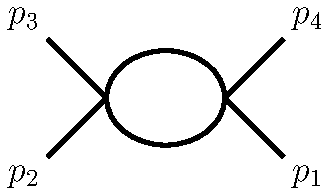
\includegraphics[width=\textwidth]{chextra_solutions/figures/boxDE_bubble_t.pdf}
$I^{\text{box}}_{0,1,0,1}$
\end{minipage}%
\hfill
\begin{minipage}{0.27\linewidth}
\centering
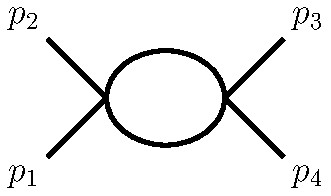
\includegraphics[width=\textwidth]{chextra_solutions/figures/boxDE_bubble_s.pdf}
$I^{\text{box}}_{1,0,1,0}$
\end{minipage}%
\hfill
\begin{minipage}{0.27\linewidth}
\centering
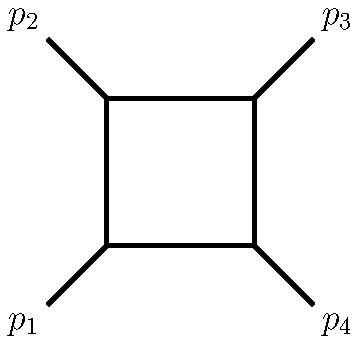
\includegraphics[width=\textwidth]{chextra_solutions/figures/boxDE_box.pdf}
$I^{\text{box}}_{1,1,1,1}$
\end{minipage}
\caption{Master integrals of the box integral family in eq.~(\ref{eq:gdef}).}
\label{fig:box_masters}
\end{figure}


\smallskip
\noindent
b) We differentiate $\vec{g}$ w.r.t.\ $s$ and $t$, and IBP-reduce the result. We obtain
\begin{align}
\begin{cases}
\partial_s \vec{g}(s,t;\eps)  = A_s(s,t;\eps)  \cdot   \vec{g}(s,t;\eps) \,, \\
\partial_t \vec{g}(s,t;\eps)  = A_t(s,t;\eps)  \cdot   \vec{g}(s,t;\eps) \,, \\
\end{cases}
\end{align}
where
\begin{align}
A_s = \begin{pmatrix}
0 & 0 & 0 \\
0 & -\frac{\eps}{s} & 0 \\ 
\frac{2 (2 \eps-1)}{s t (s + t)} &
\frac{2 (1 - 2 \eps)}{s^2 (s + t)} & 
  - \frac{s + t + \eps t}{s (s + t)} \\
\end{pmatrix} \,, \qquad
A_t = \begin{pmatrix}
-\frac{\eps}{t} & 0 & 0 \\
0 & 0 & 0 \\ 
\frac{2 (1 - 2 \eps)}{t^2 (s + t)} & 
 \frac{2 (2 \eps -1 )}{s t (s + t)} & 
 - \frac{s + t + \eps s}{t (s + t)} \\
\end{pmatrix} \,.
\end{align}
We verify the integrability conditions,
\begin{align}
A_s \cdot A_t - A_t \cdot A_s+ \partial_t A_s - \partial_s A_t = 0 \,,
\end{align}
and the scaling relation,
\begin{align}
s \, A_s + t \, A_t = \text{diag}( - \eps, - \eps , -2 -\eps ) \,.
\end{align}
The diagonal entries on the RHS of the scaling relation match the power counting of the integrals in $\vec{g}$ in units of $s$.

\smallskip
\noindent
c) We express $\vec{f}$ in terms of $\vec{g}$ as $\vec{f} = T^{-1} \cdot \vec{g}$ by IBP-reducing the integrals in \eqn{eq:fdef}.\footnote{We use the inverse of $T$ to match the convention of section~\ref{subsec:comments} for the gauge transformation.} We obtain 
\begin{align}
T^{-1} = c(\eps) \, \begin{pmatrix}
  0 & 0 & s t \\
  0 & \frac{2\eps-1}{\eps} & 0 \\
  \frac{2\eps-1}{\eps} & 0 & 0 \\
\end{pmatrix} \,.
\end{align}
The new basis $\vec{f}$ satisfies a system of DEs in canonical form,
\begin{align} \label{eq:box_canDE}
\begin{cases}
\partial_s \vec{f}(s,t;\eps)  = \eps \, B_s(s,t)  \cdot   \vec{f}(s,t;\eps) \,, \\
\partial_t \vec{f}(s,t;\eps)  = \eps \, B_t(s,t)  \cdot   \vec{f}(s,t;\eps) \,, \\
\end{cases}
\end{align}
where
\begin{align} \label{eq:boxBmatrices}
B_s = \begin{pmatrix}
\frac{1}{s + t}-\frac{1}{s} & \frac{2}{s + t}-\frac{2}{s} & \frac{2}{s + t} \\
0 & - \frac{1}{s} & 0 \\
0 & 0 & 0 \\
\end{pmatrix} \,, \qquad
B_t = \begin{pmatrix}
\frac{1}{s + t}-\frac{1}{t} & \frac{2}{s + t} & \frac{2}{s + t}-\frac{2}{t} \\
0 & 0 & 0 \\
0 & 0 & -\frac{1}{t} \\
\end{pmatrix} \,.
\end{align}
We compute $B_s$ and $B_t$ as in point b, or through the gauge transformation
\begin{align}
\eps \, B_s = T^{-1} \cdot A_s \cdot T -  T^{-1} \cdot  \partial_s T \,,
\end{align}
and similarly for $t$. From \eqn{eq:boxBmatrices} we see that the symbol alphabet of this family is $\{s, t, s+t\}$.
Thanks to the factorisation of $\eps$ on the RHS of the canonical DEs~\eqref{eq:box_canDE}, the integrability conditions split into
\begin{align}
B_s \cdot B_t - B_t \cdot B_s = 0 \,, \qquad \qquad \partial_s B_t - \partial_t B_s = 0 \,.
\end{align}
The scaling relation is given by
\begin{align}
s \, B_s + t \, B_t = -  \1_{3} \,.
\end{align}


\smallskip
\noindent
d) Viewed as a function of $s$ and $x=t/s$, $\vec{f}$ satisfies the canonical DEs
\begin{align}
\begin{cases}
\partial_s \vec{f}(s,x;\eps)  = \eps \, C_s(s,x)  \cdot   \vec{f}(s,x;\eps) \,, \\
\partial_x \vec{f}(s,x;\eps)  = \eps \, C_x(s,x)  \cdot   \vec{f}(s,x;\eps) \,, \\
\end{cases}
\end{align}
where $C_s$ and $C_x$ are related to $B_s$ and $B_t$ in \eqref{eq:boxBmatrices} through the chain rule,
\begin{align}
C_x  = s \, B_t \Bigl|_{t=x s} \,, \qquad \qquad C_s = B_s + \frac{t}{s} \, B_t \Bigl|_{t=x s} \,.
\end{align}
We observe that $C_x$  is a function of $x$ only, and $C_s$ of $s$. Thanks to this separation of variables, we can straightforwardly rewrite the canonical DEs in differential form,
\begin{align} \label{eq:box_canDEs_dlog}
\d \, \vec{f}(s,x;\eps) = \eps \, \bigl[ \d \, \tilde{C}(s,x) \bigr] \cdot \vec{f}(s,x;\eps) \,.
\end{align}
The connection matrix $\tilde{C}$ is given by a linear combination of logarithms of the alphabet letters $\alpha_1 = s$, $\alpha_2 = x$ and $\alpha_3 = 1+x$, 
\begin{align}
\tilde{C}(s,x) = \sum_{k=1}^3 C_k \, \log \alpha_k(s,x) \,,
\end{align}
with constant matrix coefficients,
\begin{align}
C_1 = - \1_{3} \,, \qquad 
C_2 = \begin{pmatrix}
  -1 & 0 & -2 \\
  0 & 0 & 0 \\
  0 & 0 & -1 \\
\end{pmatrix} \,, \qquad
C_3 = \begin{pmatrix}
  1 & 2 & 2 \\
  0 & 0 & 0 \\
  0 & 0 & 0 \\
\end{pmatrix}\,.
\end{align}


\smallskip
\noindent
e) We expand the pure integrals $\vec{f}$ as a Taylor series around $\eps=0$,\footnote{The factor $c(\eps)$ in the definition of the pure integrals~\eqref{eq:fdef} is chosen such that they are finite at $\eps=0$.}
\begin{align} \label{eq:f_eps_exp}
\vec{f}(s,x;\eps) = \sum_{w\ge 0} \eps^w \, \vec{f}^{(w)}(s,x) \,,
\end{align}
and define the weight-$w$ boundary values at $s=-1$ and $x=1$ as $\vec{b}^{(w)} = \vec{f}^{(w)}(-1,1)$.
Using \eqn{eq:Ibubblechapter4} for the bubble-type integrals we obtain
\begin{align} \label{eq:f23analytic} \begin{aligned}
& f_2(s,x;\eps) = -1+ \eps \, \log(-s) - \frac{\eps^2}{12} \left(6 \log^2(-s)-\pi^2\right) \\
& \phantom{f_2(s,x;\eps) = \, } + \frac{\eps^3}{12} \left(2 \, \log^3(-s)-\pi^2 \log(-s)+28 \, \zeta_3 \right) + \mathcal{O}\bigl(\eps^4\bigr) \,. \\
\end{aligned} \end{align}
The expression for $f_3(s,x;\eps)$ is obtained by trading $s$ for $t = s x$ in $f_2(s,x;\eps)$.
We leave $b_1^{(w)}$ as free parameters. The weight-$0$ boundary values are thus given by $ \vec{b}^{(0)} = (b_1^{(0)}, -1, -1)^{\top}$. We can now solve the canonical DEs in terms of symbols. In order to do so, we note that the canonical DEs~\eqref{eq:box_canDEs_dlog} imply the following DEs for the coefficients of the $\eps$ expansion,
\begin{align} \label{eq:box_canDEs_iteration}
\d \, f_i^{(w)}(s,x) =  \sum_{k=1}^3 \left[ \sum_{j=1}^3 (C_{k})_{ij} \, f_j^{(w-1)}(s,x) \right] \, \d \log\alpha_k(s,x) \,.
\end{align}
The iteration starts from $\vec{f}^{(0)} = \vec{b}^{(0)}$. We spelled out all indices in \eqn{eq:box_canDEs_iteration} to facilitate the comparison against the recursive definition of the symbol given by eqs.~\eqref{defsymbol1} and~\eqref{defsymbol2}. From this, we find the following recursive formula for the symbol of the solution to the canonical DEs:
\begin{align}
\mathcal{S} \Bigl( f_i^{(w)} \Bigr) = \sum_{k=1}^3 \sum_{j=1}^3 (C_{k})_{ij} \, \biggl[ \mathcal{S} \Bigl( f_j^{(w-1)} \Bigr) , \, \alpha_k \biggr] \,,
\end{align}
starting at weight $w=0$ with $\mathcal{S} \bigl( f_i^{(0)} \bigr) = b^{(0)}_i []$ (we recall that $[]$ denotes the empty symbol).
With a slight abuse of notation, we may rewrite this in a more compact form as
\begin{align}
\mathcal{S}\bigl( \vec{f}^{(w)} \bigr) = \sum_{k=1}^3 C_{k} \cdot \left[ \mathcal{S}\bigl(  \vec{f}^{(w-1)} \bigr) , \, \alpha_k \right] \,.
\end{align}
At transcendental weight 1 we thus have that
\begin{align}
\mathcal{S}\bigl(  \vec{f}^{(1)} \bigr)  = C_1 \cdot \vec{b}^{(0)} \, [s] + C_2 \cdot \vec{b}^{(0)} \, [x] +  C_3 \cdot \vec{b}^{(0)} \, [1 + x]  \,.
\end{align}
Since $[1+x]$ is the symbol of $\log(1+x)$, $\vec{f}^{(1)}(x)$ would diverge at $x=-1$ unless the coefficients of $[1+x]$ vanish. The finiteness at $x=-1$ thus implies
\begin{align}
C_3 \cdot \vec{b}^{(0)} = 0 \,,
\end{align}
which fixes $b_1^{(0)} = 4$. We now have everything we need to write down the symbol of the solution up to any order in $\eps$. For $f_1$, for instance, we obtain 
\begin{align} \begin{aligned}
& \mathcal{S}\left( f_1 \right) = 4 \, [] - 2 \, \eps \bigl( 2\, [s] + [x] \bigr)
  + 2 \, \eps^2 \bigl( 2 \, [s,s] + [s,x] + [x,s] \bigr) \\
& \, - 2 \eps^3 \Bigl( 2 \, [s,s,s] + [s,s,x] + [s,x,s] + [x,s,s] - [x,x,x]+[x,x,1+x] \Bigr) + \mathcal{O}\bigl(\eps^4\bigr) \,.
\end{aligned} \end{align}


\smallskip
\noindent
f) The dependence on $s$ is given by an overall factor of $(-s)^{-\eps}$,\footnote{The minus sign in front of $s$ ensures the positivity in the Euclidean region, where $s<0$.} which is fixed by dimensional analysis. We thus define
\begin{align}
\vec{f}(s,x;\eps) = (-s)^{-\eps} \, \vec{h}(x;\eps) \,,
\end{align}
where $\vec{h}(x;\eps)$ does not depend on $s$. We expand $\vec{h}(x;\eps)$ around $\eps=0$ as in \eqref{eq:f_eps_exp}. The coefficients of the expansion $\vec{h}^{(w)}(x)$ satisfy the recursive DEs
\begin{align} \label{eq:box_canDEs_iteration_h}
\partial_x \, \vec{h}^{(w)}(x) = \left[ \frac{C_2}{x} + \frac{C_3}{1+x} \right] \cdot \vec{h}^{(w-1)}(x) \,.
\end{align}
Equation~\eqref{eq:f23analytic} implies that
\begin{align} \begin{aligned}
& h_2(x;\eps) = -1 + \eps^2 \frac{\pi^2}{12} + \eps^3 \frac{7}{3} \zeta_3 + \mathcal{O}\bigl(\eps^4 \bigr) \,, \\
& h_3(x;\eps) = -1 + \eps \, \log(x) + \frac{\eps^2}{12} \left[ \pi^2 - 6 \, \log^2(x) \right] \\
& \phantom{h_3(x;\eps) =  \,} + \frac{\eps^3}{12} \left[ 2 \, \log^3(x)- \pi^2 \log(x) + 28 \, \zeta_3 \right] +  \mathcal{O}\bigl(\eps^4 \bigr) \,,
\end{aligned} \end{align}
which give us the boundary values $\vec{e}^{(w)} = \vec{h}^{(w)}(1)$ for the second and third integral. We have determined above that $e_1^{(0)}=4$, and we leave the remaining $e_1^{(w)}$'s as free parameters.
Integrating both sides of \eqn{eq:box_canDEs_iteration_h} gives
\begin{align} \label{eq:box_recursive_sol}
\vec{h}^{(w)}(x) =  \int_1^x \frac{\d x'}{x'} \, C_{2} \cdot \vec{h}^{(w-1)}(x') + \int_1^x \frac{\d x'}{1+x'} \, C_{3} \cdot \vec{h}^{(w-1)}(x') + \vec{e}^{(w)} \,,
\end{align}
starting from $\vec{h}^{(0)} = \vec{e}^{(0)}$. 
For arbitrary values of the undetermined $e_1^{(w)}$'s, the second integral on the RHS of \eqn{eq:box_recursive_sol} diverges at $x=-1$. We can thus fix the remaining boundary values by requiring that
\begin{align}
\lim_{x\to -1} C_3 \cdot \vec{h}^{(w)}(x) = 0 \,,
\end{align}
order by order in $\eps$.
For instance, at weight one we have that
\begin{align}
C_3 \cdot \vec{h}^{(1)}(x) = \left( e_1^{(1)} , \, 0, \, 0 \right)^{\top} \,.
\end{align}
The finiteness at $x=-1$ thus fixes $e_1^{(1)} = 0$. Iterating this up to weight 3 yields
\begin{align} \label{eq:boxDE_result} \begin{aligned}
& h_1 (x;\eps) =  4 + \eps \bigl[ - 2 \, \log(x) \bigr] + \eps^2 \biggl[ - \frac{4 \pi^2}{3} \biggr] + \eps^3 \biggl[ 
2 \, \text{Li}_3(-x) - 2 \, \log(x) \, \text{Li}_2(-x) \\
& \ + \frac{1}{3} \log^3(x)  - \log(x)^2 \log(1 + x) + \frac{7 \pi^2}{6} \log(x)   - \pi^2 \log(1 + x)  - \frac{34}{3} \zeta_3
\biggr] + \mathcal{O}\bigl(\eps^4\bigr) \,.
\end{aligned} \end{align}

\smallskip
\noindent
g) Equation~\eqref{eq:F4final} is related to \eqn{eq:boxDE_result} through $h_1 = \eps^2 s t \mathrm{e}^{\eps \gamma_{\text{E}}} (-s)^{\eps} F_4$. Up to transcendental weight two the equality is manifest. At weight three we find agreement after applying the identities
\begin{align} \label{eq:LiIdsmx} \begin{aligned}
& \mathrm{Li}_2\left(-\frac{1}{x}\right) =  - \mathrm{Li}_2(-x)-\frac{1}{2} \log^2(x)-\zeta_2 \,, \\
& \mathrm{Li}_3\left(-\frac{1}{x}\right) =  \mathrm{Li}_3(-x)+\frac{1}{3!} \log^3(x)+\zeta_2 \log(x) \,,
\end{aligned} \end{align}
for $x>0$, which we may prove by the symbol method, as discussed in chapter~\ref{sec:functionalidentitiesandsymbolmethod}.


\begin{thebibliography}{99}
%\cite{Duhr:2019tlz}
\bibitem{ch5-Duhr:2019tlz}
C.~Duhr and F.~Dulat,
``PolyLogTools \textemdash{} Polylogs for the masses,''
JHEP \textbf{08} (2019), 135
doi:10.1007/JHEP08(2019)135
[\href{https://arxiv.org/abs/1904.07279}{arXiv:1904.07279 [hep-th]}].

%\cite{Lee:2012cn}
\bibitem{ch5-Lee:2012cn}
R.~N.~Lee,
``Presenting LiteRed: a tool for the Loop InTEgrals REDuction,''
[arXiv:1212.2685 [hep-ph]].

\bibitem{ch5-website}
\href{https://scattering-amplitudes.mpp.mpg.de/scattering-amplitudes-in-qft/Exercises/}{https://scattering-amplitudes.mpp.mpg.de/scattering-amplitudes-in-qft/Exercises/}.
\end{thebibliography}